% Created 2022-05-12 jue 21:04
% Intended LaTeX compiler: pdflatex
\documentclass[12pt,letterpaper,twoside]{article}
\usepackage[utf8]{inputenc}
\usepackage[T1]{fontenc}
\usepackage{graphicx}
\usepackage{grffile}
\usepackage{longtable}
\usepackage{wrapfig}
\usepackage{rotating}
\usepackage[normalem]{ulem}
\usepackage{amsmath}
\usepackage{textcomp}
\usepackage{amssymb}
\usepackage{capt-of}
\usepackage{hyperref}
\renewcommand\maketitle{\begin{titlepage}%
\begin{center}
       \vspace*{1cm}

       \textbf{Modelo de literariedad usando redes semánticas y n-gramas}

       \vspace{0.5cm}
        
            
       \vspace{1.5cm}

       \textbf{Jonatan Ahumada Fernández}

       \vfill
            
       Tesis para el título de Ingeniería de Sistemas
            
       \vspace{0.8cm}
     
       \includegraphics[width=0.4\textwidth]{university}
            
       Facultad de Matemáticas E Ingeniería\\
       Fundación Universitaria Konrad Lorenz\\
       Bogotá, Colombia\\
       2022
            
   \end{center}\end{titlepage}%
}

\usepackage{longtable}
\usepackage[spanish]{babel}
\usepackage{float}
\usepackage{setspace}
\usepackage{mathptmx}
\usepackage{fancyhdr}
\pagestyle{fancy}
\fancyhf{}
\fancyhead[R]{\thepage}
\renewcommand{\headrulewidth}{0pt}
\usepackage{lscape}
\usepackage{booktabs}
\setlength{\parindent}{1.25cm}
\author{Jonatan Ahumada Fernández}
\date{\today}
\title{Modelo de literariedad usando redes semánticas y n-gramas}
\hypersetup{
 pdfauthor={Jonatan Ahumada Fernández},
 pdftitle={Modelo de literariedad usando redes semánticas y n-gramas},
 pdfkeywords={},
 pdfsubject={},
 pdfcreator={Emacs 27.2 (Org mode 9.4.4)}, 
 pdflang={Spanish}}
\begin{document}

\maketitle
\tableofcontents

\doublespacing
\raggedright
\setlength{\parindent}{1.25cm}





\section{RESUMEN}
\label{sec:org7105f21}

 En el presente trabajo se formula un modelo para calcular el
concepto de \emph{literariedad}, a través de dos medidas
cuantitativas: el \emph{indice metafórico} y el \emph{índicemetonímico}.
Tanto la \emph{literariedad} como la \emph{metáfora} y
la \emph{metonimia} no son conceptos \emph{ad hoc}, sino que son
modelados a partir del área de la lingüistica estructural y, en
particular, del lingüista Roman Jakobson. Luego de formular el
modelo, se evalúa a través de un diseño experimental que se basa en
el uso del Corpus de Brown. En el experimento, se corren 5 muestras
conformadas de 12 textos de categorias diferentes. Los resultados
experimentales muestran que el \emph{índice metafórico} reporta
consistentemente valores significativamente más altos para las
categorías de ficción, que era el resultado esperado. Por otro
lado, los resultados del \emph{índice metonímico} muestran
consistentemente valores más altos para las categorías de
no-ficción y en particular para los comunicados gubernamentales,
que era un resultado inesperado, pero consistente con las
teorías. El estadístico F y el valor-p de los índices apuntan a que
los resultados no son aleatorios, sino consistentes a lo largo de
las muestras.



The present work formulates a model for the concept of
\emph{literariness}, by finding two quantitative measures: the
\emph{metaphorical index} and the \emph{metonymical index}.  The
concepts of \emph{literariness}, \emph{metaphor} and \emph{metonymy}
are not \emph{ad hoc} constructs, but are modelled after the tenets
of structural linguistics and, in particular, from the works of
linguist Roman Jakobson. After formulating the model, it is evaluated
through an experimental design based on the use of the Brown
Corpus. In the experiment, 5 samples formed by 12 texts of different
categories are run.  The experimental results show that the
\emph{metaphorical index} reports values significatively higher than
non-fiction consistently, which was the expected result. On the other
hand, the results of the \emph{metonymical index} show giger values
for the non-fiction categories consistently and, in particular, for
governmental communications, wich wasn't an expected result but is
justifiable from a theoretical perspective.  The F-statistic and the
p-value for the indexes show that these results are not random, but
consistent along the samples.  

\section{FORMULACIÓN DEL PROBLEMA}
\label{sec:orgb562d6e}
\subsection{Introducción}
\label{sec:orgc299919}

¿Qué constituye la esencia de un texto? ¿Qué diferencia un texto
considerado 'literario' de aquél que no lo es? Esta pregunta se ha
planteado en áreas como los estudios literarios y la lingüística
\cite{eijembaum2010teoria}. Particularmente, la escuela denominada
'formalismo ruso' planteó que el objeto de estudio de la literatura,
no \emph{podría} ser la belleza, la relevancia histórica o el valor
pragmático de un texto. Más bien, su objeto de estudio \emph{debe} recaer
en un aspecto más 'objetivo': su \emph{literariedad}.  Como su nombre
sugiere, los formalistas se abocaron a formular una definición
'objetiva' y 'concreta' del fenómeno literario y adoptaron los --en
ese entonces-- modernos métodos de la buyente disciplina de la
linguística.

Siendo este el caso, ¿no es, por consiguiente, factible que un
autómata pueda medir y presentar tales características presuntamente
formales con las actuales herramientas informáticas? ¿Cómo se podría
traducir la noción de \emph{literariedad} a un algoritmo que pueda ejecutar
una máquina?


\subsection{Planteamiento del problema}
\label{sec:org941739e}

Roman Jakobson, en su conferencia \emph{Lingüística y poética}
\cite{jakobson1981linguistica} y en su texto \emph{Dos aspectos del lenguaje y dos
tipos de afasia} \cite{jakobson1956two} propone que la
\emph{literariedad} de un texto está dada por dos componentes del acto
linguístico: la selección y la combinación. Estos dos conceptos se
conciben como oposiciones binarias y fueron expandidos de la
teoría linguística de Saussure, que en un principio fueron
planteados como los componentes de diacronía y sincronía de la
lengua (ver figura \ref{fig:org021612c}). Puestos en el contexto del
análisis de la poesía, Jakobson renombró esos dos ejes como
\emph{metáfora} y \emph{metonímia}.



\begin{figure}[htbp]
\centering
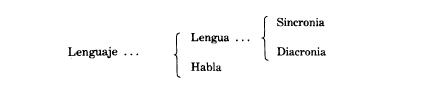
\includegraphics[width=.9\linewidth]{./assets/clasificacion_saussure.png}
\caption{\label{fig:org021612c}Distinción inicial entre sincronía y diacronía según Saussure, tomado de \cite{alonso1945curso}}
\end{figure}

¿Es posible modelar algorítmicamente tales conceptos? Según Jakobson,
en el acto de lenguaje intervienen 6 factores (ver figura
\ref{fig:orgdcd01b2}). Sin embargo, cuando se estudia la \emph{literariedad},
o la poética en general, Jakobson nos indica que nos debemos centrar
nuestra atención en el factor Mensaje: 'Esta función no es la única
que posee el arte verbal, pero sí es la más sobresaliente y
determinante, mientras que en el esto de las actividades verbales
actúa como constitutivo subsidiario y accesorio' \cite{jakobson1981linguistica}.
Así, al estudiar la \emph{literariedad} deberiamos poner un segundo plano
los aspectos que lidian con la intención (Hablante), la interpretación
(el receptor), los problemas de la lógica o referentes (Contexto) o
problemas dentro del mismo lenguaje (Código). 

La \emph{literariedad} se encuentra, entonces, en el Mensaje. En otros
términos, puede considerarse lo que está 'dentro del texto'. Aquello
que es patente.  En términos más simples: en la secuencia de sonidos
que percibimos como un mensaje, expresado a través de la palabra
escrita. Siguiendo el análisis de Jakobson, se puede teorizar que
si se considera una cadena de textos como un mensaje, podríamos
entonces hallar la \emph{metáfora} y la \emph{metonimia} y, por ende,
una medida para \emph{literariedad}.


\begin{figure}[htbp]
\centering
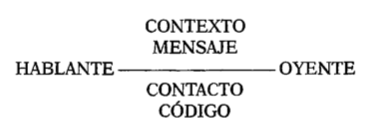
\includegraphics[width=.9\linewidth]{./assets/factores_comunicacion.png}
\caption{\label{fig:orgdcd01b2}Factores de comunicación de Roman Jakobson \cite{jakobson1981linguistica}}
\end{figure}


Las similitudes de los conceptos tanto de Saussure como de Jakobson
con las estructuras lineales y secuenciales de la computación son
evidentes a manera conceptual. Por ejemplo, en la figura
\ref{fig:orgecb6f64}, el eje AB se considera el \emph{eje de simultaneidades},
mientras que el eje CD se considera el \emph{eje de sucesiones}
\cite[pg. 106]{alonso1945curso}.

Aunque Saussure y Jakobson ofrecen un modelo cualitativo, no se halló
en la bibliografía consultada un modelo computacional que modelara el
concepto y lo implementara. Así, el objetivo de este trabajo es
modelar e implementar el modelo de \emph{literariedad} de Roman Jakobson
utilizando herramientas básicas del procesamiento del lenguaje
natural.


\begin{figure}[htbp]
\centering
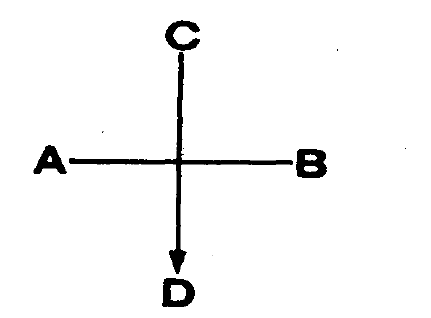
\includegraphics[width=.9\linewidth]{./assets/ejes_saussure.png}
\caption{\label{fig:orgecb6f64}Ejemplo de estructuras secuenciales en el pensamiento de Saussure. Aquí se describe prototípicamente la selección y combinación de Roman Jakobson. Tomado de \cite{alonso1945curso}}
\end{figure}

\subsection{Justificacón}
\label{sec:orgc4c8716}

En términos generales, el foco principal de la linguística
computacional han sido las aplicaciones que giran en torno a la
extracción de información, y su 'comprehensión' por parte de la
máquina. Por ejemplo, \emph{text preparation}, \emph{information retrieval},
\emph{automatic translation}, \emph{text classification}, entre otros
\cite{gelbukh2004}.

Sin embargo, las aplicaciones con un enfoque humanístico, sea este
linguístico, literario o estético son relativamente escazos, tal como
lo reportan la mayoría de autores consultados (ver sección \ref{sec:org3f83989}).  Más aún, dentro de este subcunjunto reducido, pocos
están guiados por aquello que Gelbuhk llama 'la ciencia fundamental',
la lingüistica o, desde una perspectiva de analítica de datos, la
comprensión del dominio. Más particularmente, no se encuentran modelos
que aborden los conceptos de \emph{literariedad}, \emph{selección} y \emph{combinación}
de forma explícita, a pesar de que son ideas seminales de la lingüística
de Roman Jakobson y, por ende, del llamado enfoque estructuralista.

El vacío de aplicaciones de estos conceptos es una oportunidad para
brindarle al estudio académico de la literatura herramientas basadas
en datos 'duros' o ,por lo menos, cuantitativos propias del método
científico. Por lo tanto, un modelo de la \emph{literariedad}, sustentado
en los planteamientos da lingüística diferencial, ampliaría las
aplicaciones de la lingüistica computacional y permitiría someter a
escrutinio los planteamientos de dicha teoría desde un enfoque
experimental.

Por otro lado, las escazas pero variopintas investigaciones en el área
muestran un creciente interés en calcular la 'creatividad', la 'rima'
o el 'estilo' de un texto. Sin embargo, esta misma diversidad de
enfoques evidencia al mismo tiempo una falta de cohesión entre las
disciplinas humanísticas y las ciencias (ver sección \ref{sec:org3f83989}). El autor de esta investigación cree que los conceptos de
la lingüistica estructural pueden aportar --si bien modestamente-- a
formar un mejor diálogo entre estas disciplinas y ofrecer perspectivas
que otros investigadores podrían valorar en un futuro.

Por los motivos expuestos, en esta investigación se formulará y
evaluará un modelo para obtener una medida cuantitativa para el
concepto de \emph{literariedad} de Roman Jakobson utilizando las
herramientas elementales del procesamiento de lenguaje natural y
aplicando los postulados de la linguística estructural. De este modo,
la presente investigación respondería a la pregunta ¿Cómo medir
computarizadamente la \emph{literariedad} de un texto según el marco de la
lingüística de Jakobson?

\subsubsection{\textbf{Palabras clave:}}
\label{sec:org37f819b}
NLP, computational linguistics, literariness,literary theory, poetics, theory of formal method

\subsubsection{\textbf{Área de conocimiento:}}
\label{sec:orgb49c6e4}

Lingüística computacional

\subsection{Alcances y delimitaciones:}
\label{sec:org94fe62a}

Para computar una métrica de \emph{literariedad} será necesario comparar un
\emph{corpus objetivo} con respecto a un \emph{corpus de referencia,} este
último representará el ‘uso corriente de la lengua' (ver sección
\ref{sec:org52bf584}). La primera delimitación de este trabajo es que no se
compilará un corpus propio, sino que partirá de los de acceso
libre. La mayoría de estos se encuentran en inglés. Por este motivo,
los corpus utilizados son el Corpus de Brown y Wordnet, para
que haya una congruencia de idiomas. Los criterios
utilizados para hacer los corpus comparables se detallan en la sección
\ref{sec:org8537132}.

La segunda limitación concierne a la formulación de los algoritmos en
sí mismos. Este trabajo se limitará a formular los modelos más naive
posibles.

En el caso del índice metafórico, dada una palabra, se
considerará un sinónimo todas las palabras listadas como tal en el
corpus de referencia, sin considerar los sub-problemas que esto podría
conllevar. Por ejemplo, algunos problemas podrían ser que los
sinónimos no sean suficientemente cercanos en su significado o que no
se encuentren sinónimos suficientes.

En el caso del índice metonímico, la secuencia lineal será modelada
con bigramas haciendo uso de la noción de \emph{graphic word} (ver sección
).  Es decir, se harán pares de palabras considerando cada
palabra una secuencia de caracteres separadas por un especio, sin
entrar a considerar alternativas más precisas. Por ejemplo, como
formar los n-gramas con base en sílabas o fonemas, etc.

En general, el alcance de este proyecto es formular e implementar un
modelo general que muestre cómo sería viable implementar el concepto de
\emph{literariedad}, sin ahondar en los detalles que se desprenden de cada
fase del flujo de NLP (por ejemplo, ¿cómo tokenizar?, ¿Qué peso tendrían
las diferentes partes de una oración en el computo final?, etc).

\section{OBJETIVO GENERAL}
\label{sec:org6c59e88}
Diseñar e implementar un modelo que, dado un corpus de texto, produzca
indicadores para el concepto de \emph{literariedad} que plantea Roman Jakobson.

\section{OBJETIVOS ESPECÍFICOS}
\label{sec:org2a60bd8}

\begin{enumerate}
\item Construir el corpus necesario para representar el \emph{eje diacrónico}
\item Diseñar e implementar el algoritmo para calcular la \emph{metáfora} sobre un corpus
\item Diseñar e implementar algoritmo para calcular la \emph{metonimia} sobre un corpus
\item Seleccionar y unir los textos que serán procesados (corpus objetivo) por el algoritmo
\item Correr el algoritmo sobre los corpus objetivo
\item Evaluar el algoritmo de manera cuantitativa y cualitativa
\end{enumerate}

\section{MARCO TEÓRICO}
\label{sec:orgb8c084a}

\subsection{Literariedad}
\label{sec:org10aca2d}



La \emph{literariedad} es un concepto acuñado por el lingüista Roman
Jakobson en 1919 \cite{jakobson1981linguistica}. Según el autor, es
una característica que distingue un texto considerado literario de
otro tipo de texto no literario, (como, por ejemplo, un comunicado
de prensa, un manual de instrucciones, etc):


\begin{quote}
El objeto de la ciencia de la literatura no es la literatura, sino
la literariedad (\emph{literaturnost'}), es decir, aquello que hace
de una obra determinada una obra
literaria. \cite[pg. 37]{eijembaum2010teoria}
\end{quote}

Las implicación más grande del concepto de \emph{literariedad}, es que
esta cualidad \textbf{no} depende de ningún factor extrínseco, como su
emisor, su valor histórico, sus ventas, el número de citaciones,
etc. La \emph{literariedad} se da exclusivamente por atributos
lingüísticos y, por lo tanto, es objetivamente analizable si se
utiliza el método adecuado.

Las herramientas analíticas que brinda Jakobson, son los conceptos
de \emph{metáfora} y \emph{metonímia} (ver sección \ref{sec:orgf89e914}).  Este tipo
de análisis pasó a conocerse como análisis estructuralista, porque
se basa en el estudio de presuntas estructuras existentes por debajo
de los fenómenos emergentes que, en un principio, parecen
subjetivos. En este trabajo se proponen algoritmos que producen una
medida cuantitativa tanto para la \emph{metafora} como para la \emph{metonimia}
para un texto dado. Estos conceptos se explican con mayor
detalle a continuación ( ver sección \ref{sec:orgf89e914}).


\subsection{Roman Jakobson}
\label{sec:orgf89e914}

Roman Jakobson fue un lingüista ruso americano. Se considera una
figura clave tanto en movimiento del formalismo ruso, así como en
el estructuralista.  La lingüística de Jakobson se basa en los
postulados de la lingüistica de Saussure. Sin embargo, es clave
resaltar que Jakobson propuso una crítica a las ideas de Saussure
y, en particular, postuló que los ejes de diacronía y sincronía
corresponden a 'operaciones' más profundas, que están presentes en
todo acto de habla e incluso, en todo objeto semiótico. En el
siguiente fragmento, se puede apreciar su diferencia con respecto
a Saussure:

\begin{quote}
The fundamental role which these two operations play in language
was clearly realized by Ferdinand de Saussure. Yet of the two
varieties of combination-concurrence and concatenation-it was only
the latter, the temporal sequence, which was recognized by the
Geneva linguist. Despite his own insight into the phoneme as a set
of concurrent distinctive features (\emph{éléments différentiels
des phonèmes}), the scholar succumbed to the traditional belief
in the linear character of language "which excludes the
possibility of pronouncing two elements at the same time ".
\cite[99]{jakobson1956two}
\end{quote}

La propuesta clave de Jakobson fue el concepto de \emph{literiedad}
(ver sección \ref{sec:org10aca2d}). Tal concepto se basa en un análisis
estructural de dos componentes la \emph{selección} y \emph{combinación},
también llamados \emph{metáfora} y \emph{metonimia}.

En las secciones siguientes de describirán estos conceptos, en la
medida en que apliquen al presente trabajo, puesto que, para el
lingüísta, estos dos conceptos son aplicables más ámbitos que a la
literatura.


\subsubsection{Selección (o Metáfora)}
\label{sec:org19b0ee4}

La selección o \emph{metáfora} es un principio de organización que
funciona a partir de  sustituciones. Se evidencia cuando un hablante
selecciona entre las palabras existentes de la lengua.  Por
ejemplo, para referirse a un niño, un hablante puede utilizar las
palabras 'niño', 'chico', 'jovencito', o 'párvulo', pues todas
tienen un significado similar, pero a la vez guardan una relativa
diferencia entre ellas.  Por este motivo, Jakobson
\cite[pg. 128]{jakobson1981linguistica} plantea que la selección '
tiene lugar a base de una equivalencia, similitud, desigualdad,
sinonimia y antonimia'. En otros términos, la selección se basa en
la similaridad o disimilaridad de significados.


\subsubsection{Combinación (o Metonimia)}
\label{sec:org8fa5b69}

La combinación o \emph{metonímia} es un principio de organización que
funciona a partir de relaciones de proximidad entre los signos,
cuando estos aparecen como una secuencia lineal y ordenada. Por
ejemplo, En \emph{Linguística y Poética},
\cite{jakobson1981linguistica}, Jakobson propone como ejemplo la
oracion "I like Ike". En esta se evidencia una repetición de
sonidos similares: [ay layk ayk]. La similaridad, no está dada por
el significado, sino que aquí se proyecta a lo largo del tiempo,
por la repetición de sonidos. Jakobson afirma que la combinación
'se basa en la proximidad'
\cite[pg. 128]{jakobson1981linguistica}. En términos más sencillos,
en la relación de una palabra con la que la sucede o antecede en un
mensaje.

\subsection{Poética}
\label{sec:org6c3c96f}
La poética procura responder a la pregunta de ¿qué hace que un
mensaje sea una obra de arte? Lidia principalmente con cuestiones
estéticas del lenguaje. Sin embargo, para hacer un análisis
exhaustivo, la poética debe hacer uso de la linguística, puesto
que esta última estudia el lenguaje en todo su conjunto. La
\emph{literariedad} podría, entonces, considerarse un concepto
enmarcado en la poética, porque se preguntá qué hace que un texto
sea literario y por qué es distinto de otro que no lo es.

\begin{quote}
El objeto principal de la poética es la diferencia específica del
arte verbal con respecto a otras artes y a otros tipos de conducta
verbal; por eso está destinada a ocupar un puesto preeminente dentro
de los estudios literarios.\cite[pg. 121]{jakobson1981linguistica}
\end{quote}



\subsection{Estructuralismo}
\label{sec:org11edf5f}

El \emph{estructuralismo} se entiende como un método utilizado entre
varias disciplinas humanísticas, como literatura, antropología e
historia, entre otras.  Se considera que el origen del movimiento
estructuralista fueron las ideas de la lingüística de Saussure
(). Hay, por lo tanto, diversos objetos de estudio
sobre los cuales se les puede aplicar el método estructuralista.
Gerard Genette, en \emph{Estructuralismo y Crítica Literaria}, delimita
los alcances y delimitaciónes del método:

\begin{quote}
 (..) el estructuralismo como método está destinado al estudio de las
estructuras en todas partes donde se las encuentra; pero, en
principio, las estructuras, por mucho que se quiera, no son objetos
que se encuentran sino sistemas de relaciones latentes, concebidos más
bien que percibidos, que el análisis construye a medida que los
desentraña y que a veces corre el riesgo de inventar creyendo
descubrirlos.  \cite[pg. 145]{genette1996estructuralismo}
\end{quote}

En el marco de este trabajo, las estructuras a estudiar se limitan
a la \emph{metáfora} y la \emph{metonimia} (ver \ref{sec:orgf89e914}), que son
las que el juicio experto propone como más importantes. Ahora
bien, es pertinente resaltar que, como se evidencia en algunos
trabajos del marco referencial, los problemas del estructuralismo
son similares a los problemas de los modelos no-supervisados de
Machine Learning. Por ejemplo, el estructuralismo pregunta ¿qué
relaciones en el objeto de estudio son las más pertinentes para
analizar? y en el machine learning se pregunta ¿cuáles son las
características (features) que producirán una mejor predicción? Y
en el caso de los modelos no supervisados, existe un debate acerca
de qué interpretación darle a las medidas escogidas por el
algoritmo \cite{van2019vector}.
\subsection{Linguística}
\label{sec:orgaa8a326}

La lingüística es la ciencia que estudia el lenguaje.
Tradicionalmente, esta ciencia se subdivide en las ramas de fonética,
fonología, morfología, sintaxis, semántica y pragmática. \cite{gelbukh2004}

La lingüística es un campo de estudio interdisciplinar e involucra
disciplinas heterogéneas como la lógica y la neurolingüistica. Sin
embargo, se considera que hay un núcleo común llamado \emph{linguística
general}.

\subsubsection{Lingüística General:}
\label{sec:org9617945}

Se conoce como lingüística general al paradigma lingüístico
establecido por Ferdinand De Saussure, también llamado \emph{modelo
diferencial del lenguaje}.

El modelo diferencial se caracteriza porque propone dos ejes
principales existentes en la lengua: el \emph{eje de sincronía} y el
\emph{eje de diacronía}.\cite{alonso1945curso}

Estos dos ejes son la base de lo que Jakobson considera \emph{selección} y
\emph{combinación}.


\subsubsection{Lingüística sincrónica}
\label{sec:orgd28e7a5}

Cuando Saussure habla de lingüística sincrónica, se refiere al
estudio del estado actual de la lengua, sin tener en cuenta los
cambios históricos de esta. Luego, la linguística sincrónica lidia,
por ejemplo, con las formas en que los hablantes vinculan los
signos (significantes) con los significados a través de reglas de
sintaxis, de pronunciamiento, de léxico, etc. Sin embargo, el
estudio diacrónico tiene en cuenta que esto solo aplica para
ese instante particular y siempre se tiene en cuenta la relación
con el \emph{eje diacrónico}. En la perspectiva de Jakobson, el eje de
sicronía pasa a ser la selección (ver seleccion en ).

\subsubsection{Lingüística diacrónica}
\label{sec:org972b810}

La linguística diacrónica estudia los cambios sucesivos en la
lengua, producidos por la actividad constante del \emph{eje
sincrónico}. Saussure plantea en un principio a la lingüistica
diacrónica como el estudio de los cambios históricos de la
lengua \cite{alonso1945curso}.


Sin embargo, en la perspectiva de Jakobson, un \emph{mensaje} tiene en
sí mismo un eje diacrónico (ver combinación en ).
como secuencia. 

\subsection{Lenguaje}
\label{sec:org47ca62a}
En términos simples, el lenguaje es la facultad de formular y
comprender signos o símbolos, ya sean hablados, escritos,
imágenes, etc.  En otros términos, el lenguaje es una capacidad
general. Sin embargo, para Saussure, el lenguaje tiene una
característica doble: que es al mismo tiempo un sistema
establecido y la constante evolución de tal sistema. Estos dos
componentes son la \emph{lengua} y el \emph{habla}.

\subsubsection{Lengua}
\label{sec:org52bf584}

La lengua (\emph{langue}) es uno de los dos componentes del
\emph{lenguaje}.  La lengua es fenómeno social y se equipara a una
\emph{cristalización} o un producto de la suma de asociaciones entre
conceptos e imagenes acústicas en la mente de los hablantes. Por
ejemplo, la lengua es lo que permite que dos hablantes bogotanos
puedan asociar en su mente el sonido de la palabra 'chino' con el
concepto de 'niño' o 'infante', mientras que en otras partes del
mundo hispanohablante no existe tal asociación común.  En
términos simples, la lengua es un entendimiento compartido de lo
que significan las palabras \cite[pg. 102]{alonso1945curso}. La
contraparte de la \emph{lengua}, es el \emph{habla} .

\subsubsection{Habla}
\label{sec:orga69a402}
El habla (\emph{parole}) es uno de los dos componentes del
\emph{lenguaje}. El habla es el uso individual de la lengua.
Evidentemente, cuando un individuo habla puede modificar
la lengua a su antojo, porque posee la facultad del
lenguaje y jamás meramente repite el consenso de la lengua.
Como consecuencia de esto, la lengua está continuamente
siendo transformada por el habla. En términos simples,
la suma de los actos individuales de comunicacion lentamente
terminan por transformar el consenso social sobre cómo
hablar.  Por este motivo la linguística debe tener una
perspectiva doble: \emph{diacrónica} y \emph{sincrónica}.


\subsection{Lingüística Computacional}
\label{sec:org63f6365}

Es la intersección entre la computación y la lingüística. Por lo
general, se preocupa por cómo procesar automáticamente el
lenguaje natural, para lo cual genera modelos lingüísticos sobre los
que luego se pueden definir operaciones comunes \cite{gelbukh2004}.


La lingüística computacional es en sí misma un campo amplio y
heterogéneo(ver \ref{fig:orgf3447fb}).
Este trabajo se incribe concretamente dentro del procesamiento
del lenguaje natural \ref{sec:orgcb37299}, y tiene un fuerte componente de
lingüística general .

\begin{figure}[htbp]
\centering
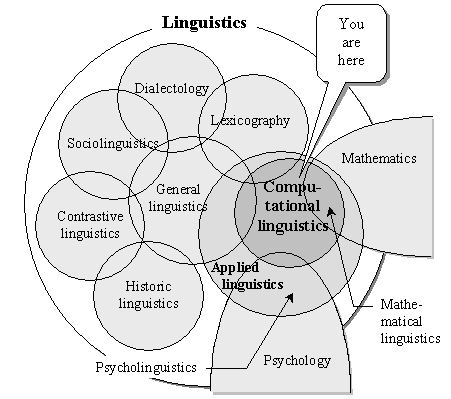
\includegraphics[width=.9\linewidth]{./assets/mapa_linguistica.png}
\caption{\label{fig:orgf3447fb}Relación de linguística computacional con otras areas tomado de \cite{gelbukh2004}}
\end{figure}


\subsection{NLP}
\label{sec:orgcb37299}
El procesamiento del lenguaje natural (NLP, por sus siglas en
inglés), es a menudo considerado sinónimo con la lingüística
computacional \cite{gelbukh2004}.  Sin embargo, el NLP se refiere
concretamente a la aplicación práctica de la linguística
computacional para procesar automáticamente) mensajes (a menudo en
enormes cantidades) de lenguaje natural y obtener de estos alguna
información o un acción sin intermedio de un humanano.

En este trabajo, se utilizan algunas herramientas típicas del
NLP, como corpus, N-gramas, tokenización y vectorización, explicadas
en a continuación. Sin embargo, es necesario hacer explítico de
que se parte una herramienta computacional en particular: NLTK.

\subsubsection{NLTK}
\label{sec:org88564fb}
El Natural Language Toolkit (NLTK) es un módulo de Python que ofrece
una interfaz para tareas comunes en la lingüística computacional. La
ventaja principal de NLTK es que se considera a sí mismo un
\emph{toolkit}. Esto significa que no impone una estructura de
procesamiento definida, sino que a ofrece un extenso abanico de
herramientas, tales como: tokenizacion, filtros, generación de
n-gramas, análisis sintáctico de oraciones, entre otras.

Se seleccionó esta herramienta porque no impone una estructura
rígida en cuantó que cómo procesar el texto, lo que la hizo
idónea para perseguir los objetivos interdisciplinares de esta
investigación. En cuanto a las herramientas concretas utilizadas,
se expondrán a continuación.

\subsubsection{N-gramas}
\label{sec:org974f038}

Los N-gramas son una herramienta común en el procesamiento
de lenguaje natural y tienen diversas aplicaciones. Desde sus
inicios \cite{manning1999foundations}, los n-gramas se han
utilizado para capturar la noción de 'contexto' o 'historia'
dentro de una secuencia de tokens. Así los n-gramas, forman
una tupla o secuencia de palabras dentro de una secuencia
o texto más grande y, delimitado el tamaño o nivel del
n-grama, los términos circunscritos dentro del n-grama
se entienden como variables aleatorias dependientes entre sí.

Así, los n-gramas se utilizán para tratar de predecir alguna
característica con base en algún otro componente del n-grama,
utilizando las teorías de cadenas de Markov.

En este trabajo, los n-gramas se utilizan meramente
como una herramienta que captura la 'memoria' o 'relación'
de dos palabras adyacentes dentro de un mensaje. No se
utilizarán funciones de probabilidad, sino que se hará
un cálculo de similitud utilizando el algoritmo descrito
en la sección  \ref{sec:orgca3f630}, utilizando
n-gramas de nivel 2 o \textbf{bigramas}.


\subsubsection{Tokenización}
\label{sec:org2db9112}
La tokenización es el proceso mediante el cual se separa la entrada
de un programa NLP en unidades de análisis más pequeñas llamadas
\textbf{tokens}. Un token puede ser una palabra, aunque no necesariamente
lo es. Por ejemplo, puede ser un lexema, un signo de puntuación
o una unidad sintáctica (un constructo sujeto - verbo, por ejemplo)
\cite{manning1999foundations}. El resultado de la tokenización
dependerá, por lo tanto, de los objetivos de la investigación.

En esta investigación se tokenizará siguiendo la noción de
palabra gráfica (\emph{graphic word}). Esto simplemente se refiere
a que cada token corresponde a una palabra separada por un espacio,
incluyendo signos de puntuación y otros caracteres alphanumericos.




\subsubsection{Vectorización}
\label{sec:orge7117de}
La vectorización es el proceso de tomar una característica o medida
y representarla como una secuencia números reales, como un vector. A menudo,
tal representación permite visualizar las características en un espacio
vectorial, aunque la visualización no es la ventaja crucial.

La vectorización es una técnica utilizada a lo largo de muchos
dominios y tiene una larga historia en el proceso de transformar
un concepto a una entrada que sea interpretable por una máquina
\cite{jha_abhishek_vectorization}.  Continuamente, catalizadas por
el auge del Machine Learning, se desarrollan técnicas de
vectorización que ayudan a hacer los cálculos de similitud entre
vectores más eficientes, dependiento del objetivo. Un buen
ejemplo es el desarrollo del modelo de Google, que
codifica las palabras de tal forma que agiliza el cálculo
de similitud entre conceptos, conservando la noción
de múltiples grados de similaridad \cite{mikolov2013efficient}.

En este trabajo, la técnica de vectorización utilizada es
la \emph{bag of words}, que es una técnica basada en la \textbf{frequencia}.

\subsubsection{Bag of words}
\label{sec:org080183f}

Es una técnica de vectorización frecuentemente utilizada en NLP.
Se considera de complejidad sencilla, pero funciona exitosamente
en muchos casos de uso. Involucra 3 fases: tokenización, creación de vocabulario y,
finalmente, creación del vector.

Su funcionamiento es el siguiente: una vez se tiene el la entrada
tokenizada se construye un \emph{vocabulario}.  Este es set de cada
palabra utilizada en la entrada.  Luego, se procede a asociar a
cada palabra del vocabulario a su frecuencia en el texto, con lo
cual se obtiene un histograma de palabras. En la última etápa,
usualmente se utiliza una matriz llana en la que cada fila
corresponde con una oración y cada columna representa una entrada
en el vocabulario \cite{jha_abhishek_vectorization}.

No obstante, para en este trabajo no se utilizará este enfoque
tradicional.  Sino que el proceso de vectorizacións seguirá los
pasos descritos en la sección \ref{sec:orgca3f630}. Sin embargo,
es necesario mencionar que la técnica de bag of words conlleva
a los siguientes supuestos: 1) se asume que el orden de las
palabras en la entrada no importa, tan solo la frecuencia
de cada entrada y 2) la existencia de las palabras en el
vocabulario es indenpiente una de la otra.  
\subsubsection{Corpus}
\label{sec:org53a56e6}


Un corpus es una colección de textos auténticos que pueden ser
leídos por una máquina. Estos pueden estructurarse de muchas
formas, dependiendo de los objetivos de la investigación
\cite{indurkhya2010handbook}. Por ejemplo, pueden ser aislados (una
colección arbitraria), categorizados (una colección escogida según
algún criterio), temporales (una colección organizada
cronológicamente) o solapados (un documento puede pertenecer a
varias colecciones) \cite{bird2009natural} (ver figura
\ref{fig:org6a3dd54}). Además, el formato del corpus varía
significativamente de acuerdo al objeto de la investigación. Por
ejemplo, si se desea hacer un análisis sintáctico (de la estructura
de una oración), se debe hacer un corpus anotado con POS (Part Of
Speech tag); para hacer un análisis pragmático se utiliza una
anotación pragmática, etc.



\begin{figure}[htbp]
\centering
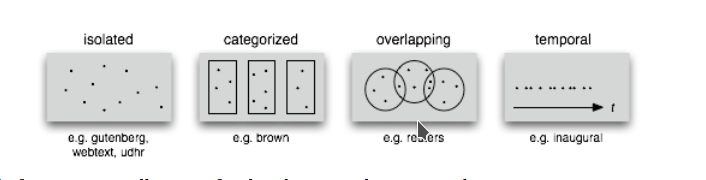
\includegraphics[width=.9\linewidth]{./assets/estructuras_de_corpus.png}
\caption{\label{fig:org6a3dd54}Diferentes estructuras de corpus}
\end{figure}

\subsection{Analítica de datos}
\label{sec:org8962c76}
La analítica de datos es una disciplina heterogenea que auna
diversas áreas de de estudio, como la teoría de la computación, la
estadística, los negocios y cualquier otro dominio sobre el cual es aplicada
(por ejemplo, química, biología, etc).  Una forma sucinta de
entender la analítica de datos es el proceso mediante el cual se
extrae \textbf{información} de los \textbf{datos} \cite{nelli2018python}. Así,
se entiende por dato un registro que representa una medida de
algún fenómeno observable. Por otro lado, la información se
entiende como el conjunto de conclusiones aplicables que se
obtienen de los datos luego de ser procesados. Tal proceso es
el que se conoce como \textbf{análisis de datos}. El análisis
de datos es variado y utiliza distintos recursos estadísticos
y matemáticos, pero por lo general la análitica de datos
tiene por objetivo generar un \emph{modelo} de los datos
que tenga capacidad \emph{predictiva}.

Como se ve, la análitica de datos provee, más que un resultado
concreto, una metodología para obtener modelos. Este trabajo,
por lo tanto, se enmarca dentro de la analítica de datos
en la medida en que se propone un modelo y lo evalua haciendo
uso de rasgos comunes como: el uso de repositorios de datos
(corpus), el uso de la estadística descriptiva para evaluar
el modelo, la formalización de un modelo en términos matemáticos
y el uso del stack de analítica de datos de Python (Pandas, Numpy,
Seaborn, ScikitLearn).

Ahora bien, si bien en este trabajo se enmarca dentro de la
analítica de datos, se debe aclarar que el modelo presentado
\textbf{no} es producido a partir de ninguna técnica  de Machine Learning.

En cuanto a la información específica de la metodología, este
proyecto se guió por la metodología CRIPS-DM

\subsection{CRISP-DM}
\label{sec:org4043321}
El Cross Industry Standard Process for Data Mining (CRISP-DM) es
un modelo que sirve de base para cualquier proceso de analítica de
datos. Este consta de 6 fases: 1) Entendimiento del negocio (¿Qué
necesita el negocio?), 2) Entendimiento de los datos (¿Qué datos
tenemos/necesitamos?¿Se necesitan limpiar?), 3) Preparación de los
datos (¿Cómo organizamos los datos para modelar?), 4) Modelamiento
(¿Qué técnicas de modelamiento deberíamos aplicar?), 5) Evaluación
(¿El modelo cumple con los objetivos de negocio?) y 6) Despliegue
(¿Cómo acceden a los resultados los interesados?)
\cite{wirth2000crisp}.

CRISP-DM se utiliza, por lo tanto, como una guía para
asegurar que cada fase del proceso de análitica de datos
tenga las consideraciones adecuadas. Así el Diseño Metodológico
de este trabajo está organizado según las fases mencionados.
Sin embargo, cabe aclarar que algunas modificaciones debieron
ser hechas a las fases, sobre todo a lo concerniente con las
fases de Evaluación y Despliegue, pues el objetivo de este
trabajo no es producir un modelo utilizado en un entorno empresarial.



\section{MARCO REFERENCIAL}
\label{sec:org3f83989}

En la revisión de la literatura se encontraron, a groso modo,
dos tipos de trabajos que se consideran antecedentes cercanos. Esta
distinción es importante porque cada categoría tiene un enfoque
distinto sobre el problema de la \emph{literariedad}. A continuación,
se presentarán estos dos tipos (Tipo I y II)  de trabajo y se mencionarán los
aspectos relevantes para el presente trabajo. 


\subsection{Tipo I}
\label{sec:org5943744}
El primer tipo de trabajo tiene un enfoque basado en \emph{Machine
Learning}, tienen un componente explorativo, y los autores por lo
general se muestran escépticos al concepto de \emph{literariedad}. Dentro
de estos, los más relevantes son los de Cranenburgh
\cite{van2019vector} \cite{van2015identifying} y Louwerse
\cite{louwerse2008computationally}. En ambos trabajos los autores
hacen una alusión explícita al concepto (\emph{literariness}). No obstante,
estos dos trabajos pasan por alto las bases linguísticas del concepto
y se presenta la \emph{literariedad} como una medida percibida por el
lector, y poco articulada. Por ejemplo, Cranenbourgh afirma:

\begin{quote}
However much debated the topic of literary quality is, one thing we do
know: we cannot readily pinpoint what ‘literary’ means. Literary
theory has insisted for a number of years that it lies mostly outside
of the text itself (cf. Bourdieu, 1996), but this claim is at odds
with the intuitions of readers, of which the
\cite[pg. 58]{van2015identifying}
\end{quote}


De igual forma, Lowerse coincide y menciona:


\begin{quote}
(\ldots{}) whether literary texts overall are linguistically different from
non-literary texts is a question that has not been satisfactorily
answered.\cite[pg. 176]{louwerse2008computationally}
\end{quote}

Como es evidente, la presente investigación toma el enfoque opuesto a
estos trabajos previos. En concreto: en la presente se parte del
supuesto de que la \emph{literariedad} está suficientemente descrita por
Roman Jakobson y que es algo 'dentro del texto', no dependiente de
apreciaciones subjetivas. Por consiguiente, se suspende el juicio con
respecto a los contra-argumentos usuales en contra de la
\emph{literariedad} \cite{chuit2019epistemologia}, el \emph{formalismo} o, de
manera más generalizada, el \emph{estructuralismo} y se aboca a proponer y
validar un modelo.

La otra divergencia del presente trabajo con respecto a este primer
tipo, se da a nivel del uso de tecnologías. En el presente trabajo no
se hace uso de Machine Learning, entendiendo este término como el uso
de modelos bayesianos (Latent Dirchlet Allocation), modelos de
regresión lineal (Suppport Vector Machines) o redes neuronales
(Paragraph Vectors).

Consiguientemente, en los trabajos citados (exceptuando a
\cite{louwerse2008computationally}), se entiende la literariedad como
aquellos patrones que producen la classificación más apta. En el
presente trabajo, en contraparte, se formula un modelo basado en la
teoría y luego se evalua experimentalmente. Se podría decir, a manera
de síntesis, que en los trabajos de tipo I la \emph{literariedad} se
encuentra. En este trabajo, en cambio, la \emph{literariedad} se modela.



\subsection{Tipo II}
\label{sec:org89d8503}
Ahora bien, el segundo tipo de trabajo tiene un enfoque basado en
estadística y vectorización, pero no emplea de forma explícita el
concepto \emph{literariedad} u otra fundamentación de la linguística
saussureana. Sus inicios, segun Blei, inician en
\cite{klarreich_2019}. En los trabajos de este tipo, los autores,
partiendo de un interés muy delimitado buscan medir una característica
concreta: determinar el orígen de un texto \cite{klarreich_2019},
obtener una herramienta de visualización gráfica
\cite{kaplan2006computational}, determinar el grado de creatividad de
una traducción \cite{zuniga2017automatic} o, en términos más
generales, capturar el \emph{estilo} \cite{delmonte2005venses}
\cite{delmonte2013computing}.


Su característica principal es que proponen una extensa lista de
medidas posibles sobre un texto, forman un espacio vectorial y luego
hacen uso de alguna técnica de reducción de dimensionalidad (Principal
Component Analysis, Support Vector Machines). Dentro de este tipo de
trabajo, el más relevante es Kaplan Blei, en cuyo primer trabajo
\cite{kaplan2006computational} de tesis de pregrado visualiza 84
métricas distintas en un espacio vectorial y luego formaliza en un
artículo científico. \cite{kaplan2007computational}.

Los trabajos de Kaplan, son luego citados por el trabajo de Delmonte
\cite{delmonte2013computing} \cite{delmonte2005venses}. La trayectoria
de Delmonte es bastante amplia en su alcance. Iniciando con módulos
que calculan similaridades semánticas en un texto \cite{delmonte2005venses},
luego aprovecha las ideas de Kaplan para desarrollar un sistema multi-modular
que abarca prácticamente todas las áreas de estudio de la linguística:
semántica, fonética, gramática e incluso aspectos que tienen que ver
con la rima (prosodia).

A pesar de el trabajo de Delmonte es el más rico y complejo no solo
dentro de este tipo, sino de toda la bibliografía consultada,
realmente nunca hace alusión al concepto de \emph{literariedad}. Lo más
relevante del trabajo de Delmonte es el uso constante de las mismas
herramientas (tokenizadores, splitters, n-gramas y NER) para construir
módulos de creciente complejidad. 


El aporte principal de Delmonte fue su innovación al momento de
aplicar herramientas comunes de NLP (tokenizadores, splitters y NER)
con el fin de analizar aspectos a lo largo de las distintas áreas de
la lingüistica. Por lo tanto, sus modelos son mucho más informados y
propone soluciones a aspectos complejos del análisis lingüístico que los
autores anteriores no abordan.

Por último, dentro de este segundo tipo de trabajo, tiene mención
especial el trabajo de \cite{zuniga2017automatic}. Aquí se establece
una métrica para medir el grado de creatividad en la poesía, basándose
en qué tanto de la rima se conserva en la traducción de un poema con
respecto al original. De aquí se tomó la idea de establecer una
métrica para un aspecto tradicionalmente cualitativo (la creatividad),
desde una perspectiva \emph{hand-crafted}. Lo que diferenció este trabajo
del de Delmonte, es su aproximación matemática. Aquí se proveen
fórmulas para cada una de las 7 medidas propuestas. El grado de
complejidad para cada medida es sencillo, pero se obtienen buenos
resultados.  Lo que fue un ejemplo tremendo para este trabajo, pues
muestra las ventajas del \emph{hand-crafted features}, en contraposición al
de \emph{learned-features}. Esto destacó el valor de formular medidas
propias por sobre las de un algoritmo no supervisado.

\section{DISEÑO METODOLÓGICO}
\label{sec:org0ffb4c5}
El diseño metodológico seguirá --a grandes rasgos-- los pasos de la
metodología CRISP-DM, que se considera un estándar \emph{de facto} para
proyectos de minería de datos. Esta metodología ayudará organizar
el proceso de mi investigación, que vá desde el acceso a los corpus
(los datos disponibles) hasta el despliegue (la visualización de
los resultados).

\subsection{Entendimiento del negocio}
\label{sec:org9f1292d}

El resultado tangible del modelo de literariedad propuesto son dos
métricas cuantitativas: \emph{metáfora} y \emph{metonímia}.  Estas métricas
juntas constituiran una representación 'objetiva' del concepto
cualitativo de \emph{literariedad}.

\begin{figure}[htbp]
\centering
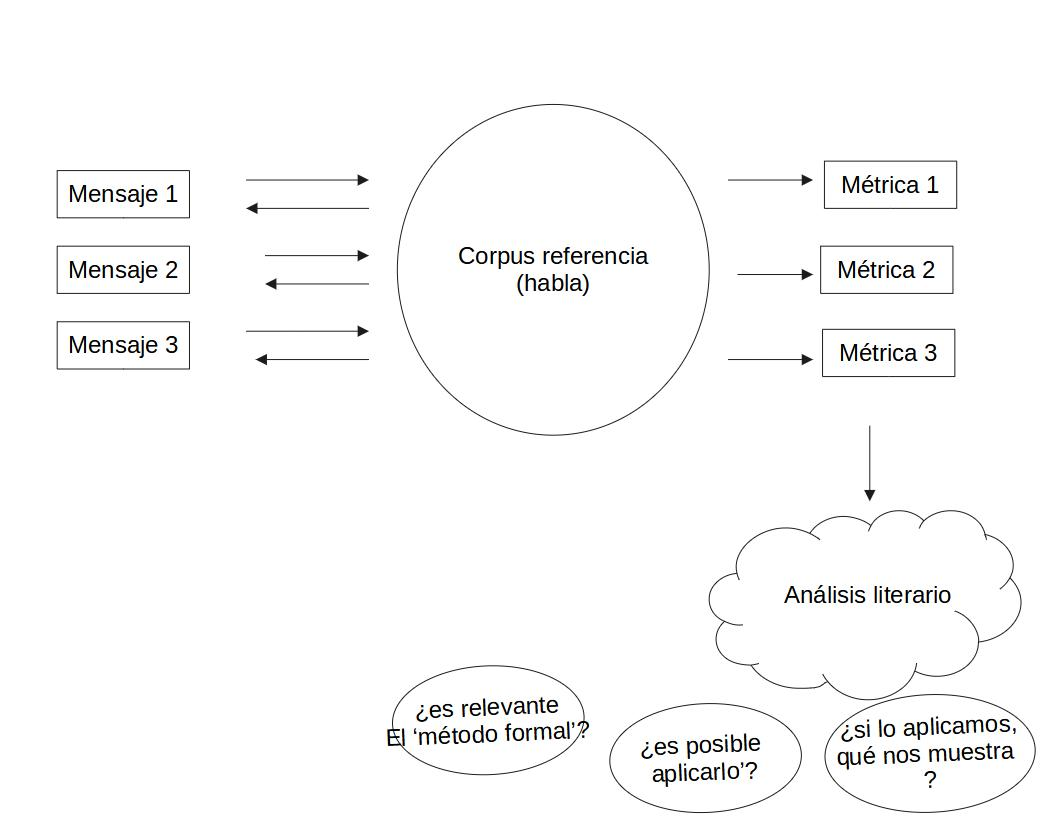
\includegraphics[width=.9\linewidth]{./assets/posibles_usos.jpg}
\caption{\label{fig:posibles_usos}Entradas y salidas del algoritmo}
\end{figure}


¿Cuál sería el beneficio de obtener este resultado? Se podría
comparar las métricas de \(n\) mensajes cualesquiera y tener una
medida objetiva con las cuales compararlas. Algunos casos de uso
posible serían:

\begin{itemize}
\item determinar si un mensaje personal que he escrito es más
metáforico o metonímico que otro,

\item determinar si un mensaje de una misma categoria (por ejemplo,
del mismo autor, o del mismo género) tienen medidas de metáfora
y metonímia similares,

\item comparación literaria, por ejemplo, poemas de la escuela
simbolista y compararlo con poemas realistas y verificar si
hay o no una diferencia sustancial desde el punto de vista
linguístico,
\end{itemize}

Como se puede apreciar en la figura , las aplicaciones
del modelo en principio supondrían un factor adicional para ser
considerado para el estudio literario, cuya naturaleza es
cualitativa. Sin embargo, si el modelo demuestra ser efectivo,
podría llegar a ser una medida de similitud para un texto, lo que
implicaría que se podría clasificar un texto con base en su
metáfora y metonímia.


\subsection{Entendimiento de los datos}
\label{sec:orgb62e61f}

En esta sección, se enumeran las distintas fuentes de datos o
recursos, que en este caso vendrían a ser los diferentes tipos de
corpus necesarios para el modelo. Cada fuente se utiliza para
formar un componente dentro del modelo (nivel de abstracción), que
guarda una relación con la teoría lingüística.  Estas relaciones
están sintetizadas en la figura \ref{fig:orgee8172c}.
A continuación, se describe cada tipo de dato, vinculándolo con su
recurso, la tecnología implicada y la teoría.

\begin{figure}[htbp]
\centering
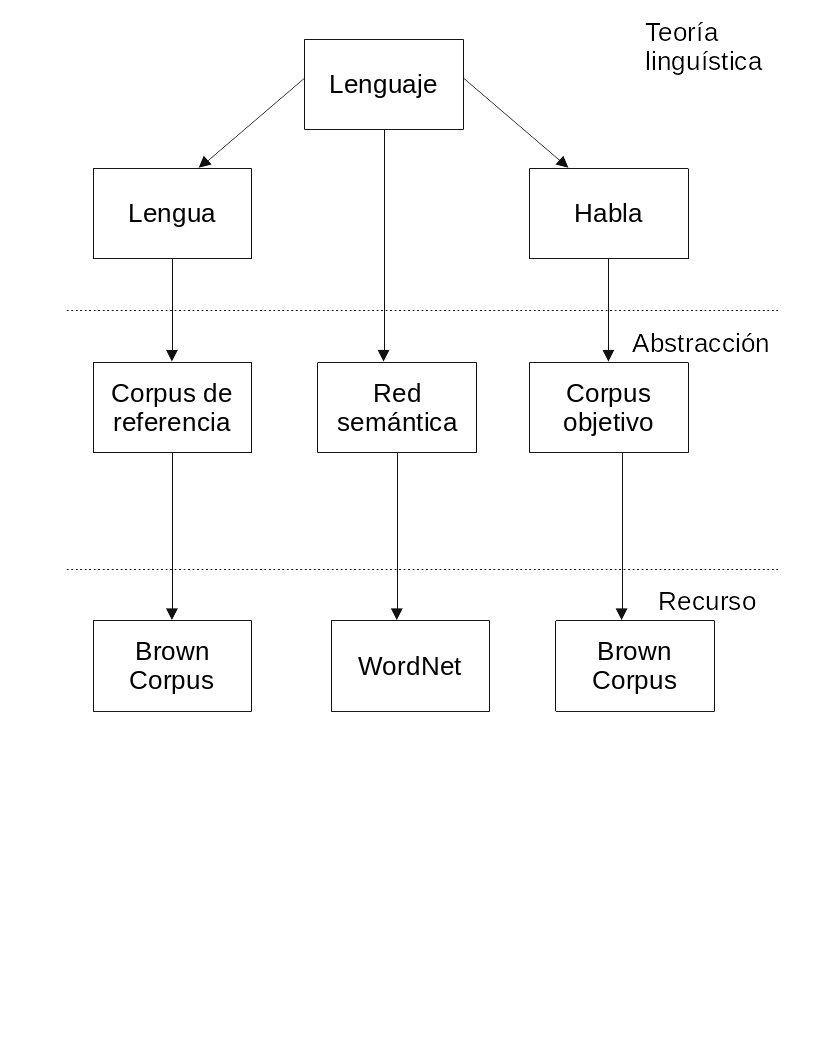
\includegraphics[width=.9\linewidth]{./assets/entendimiento_de_los_datos.png}
\caption{\label{fig:orgee8172c}Resumen de las fuentes de datos utilizadas para cada concepto}
\end{figure}



\subsubsection{El corpus de referencia}
\label{sec:orgf706c36}

El corpus de referencia es un compendio de muestras textuales que
representa un consenso sobre el uso de la \emph{lengua}
(ver \ref{sec:org52bf584}). Su correlación teórica es el eje de diacronía (ver
\ref{sec:orgd28e7a5}) y cumple la función de cristalizar una
lengua en un lugar y un tiempo establecido.

Desde un punto de vista técnico, es una cadena de texto de
longitud arbitraria sobre la cual se forma una bolsa de palabras
(ver \ref{sec:org080183f}) basada en frequencias.

Como fuente del corpus de referencia, se utiliza el Corpus de
Brown. El Corpus de Brown se accede a través de la librería NLTK
de Python (ver \ref{sec:org88564fb}), que provee una descarga asistida a través
de su módulo `nltk.corpus`.


\subsubsection{El corpus objetivo}
\label{sec:orgea754f2}

El corpus objetivo serán los mensajes sobre los cuales se
computarán las dos medidas de \emph{metáfora} y \emph{metonimia}.  Su
correlativo teórico es el \emph{habla} y son los textos que el usuario
final del final del sistema desea someter a análisis.

A nivel técnico, cada mensaje es una sola cadena de texto de
longitud arbitaria.

Como fuente de los corpus objetivo, también se utiliza el Corpus
de Brown, puesto que, siguiendo los postulados de la teoría, el
\emph{habla} se debe estudiar en relación con la \emph{lengua}. Los
detalles sobre qué téxtos específicos del Corpus de Brown son
utilizados como corpus objetivo están detallados en la sección
\ref{sec:org8537132}.



\subsubsection{La red semántica}
\label{sec:org5d724f7}

La red semántica es un componente que permite vincular palabras
entre sí en virtud de su significado. Su correlativo teórico
es la noción de lenguaje mismo, entiendo por este la facultad
de comprender sistemas de signos (ver \ref{sec:org47ca62a}).

A nivel técnico, la red semántica no se preparará o implementará
de ningún modo, sino que se utilizará el recurso WordNet. WordNet
es una base de datos léxica que, entre sus muchas aplicaciones,
puede funcionar como red semántica porque provee sets de
sinonimos (llamados \emph{synsets}) para las palabras
\cite{fellbaum_1998}. El accesso a la WordNet también lo provee la
libreria NLTK a través de su módulo `nltk.corpus`.



\subsection{Preparación de los datos}
\label{sec:org8537132}
\label{sec:preparacion_datos} La tarea de preparación de los datos
consiste principalmente en seleccionar confeccionar los corpus
necesarios para el modelo (corpus de referencia y corpus objetivo)
a partir del corpus de Brown, seleccionando cada los textos de
manera significativa y coherente.  A continuación, se describen los
criterios utilizados para realizar la selección de textos.

\subsubsection{Corpus de referencia}
\label{sec:orgac22997}

El corpus de referencia representa la \emph{lengua} (\emph{langue}). Por lo
tanto, debe estar compuesto de una muestra de textos
comparativamente mucho más grande los mensajes individuales que
serán contrastados con este. ¿Cómo construir un corpus tal?

En primer lugar, se descartó la idea de modelar la \emph{lengua} en su
totalidad, pues como lo indica la teoría linguística, esta tarea
es imposible puesto que esta se encuentra en constante
cambio. Así, el primer criterio para construcción del corpus fue
restringirlo diacrónicamente al espacio de un año y a un idioma
específico.

El siguiente criterio fue armar un corpus \emph{balanceado}. Es decir,
el corpus de referencia no puede estar compuesto de muestras de
un mismo tipo (un estilo, un género, un autor), porque esto
sesgaría la comparación de el corpus objetivo con respecto a
este. Así, se optó por partir de un corpus \emph{categorizado} y tomar
partes iguales de cada una de las categorias. Esto es, cada
categoría tiene igual peso en cuanto a número de textos y
palabras que lo representan.

El tercer criterio fue utilizar un corpus fácilmente accesible,
de origen libre y avalado por la comunidad científica. Por todos
los motivos anteriores, se escogió el corpus de Brown, que
presenta las siguientes características:

\begin{itemize}
\item todas las muestras del corpus pertenecen al año 1961,
\item todas las muestras del corpus se imprimieron en Estados Unidos durante ese año,
\item todos los autores son hablantes nativos de inglés,
\item la categorización de las muestras fue hecha por un comité de expertos de la universidad de Brown,
\item la intención declarada del corpus es la de ser una muestra representativa del inglés de aquel año,
\item tiene una lista amplia de categorías que podrían ser útiles para observar diferencias entre las categorías,
\item el número de textos por categoría guarda la relación entre los textos publicados de esa categoría durante ese año y
\item los resultados obtenidos del modelo podrían ser replicados porque el corpus es ampliamente conocido.
\end{itemize}

En la tabla \ref{tab:corpus_referencia} se muestra lo que se
utilizará como corpus de referencia.


\small

    \begin{longtable}[c]{| p{.05\textwidth} | p{.40\textwidth} | p{.20\textwidth}|} 
    \hline
        cód.  & nombre  & categoria  \\ \hline
        a01 & Political Reportage & reportage  \\ \hline
        a11 & Sports Reportage & reportage  \\ \hline
        a19 & Spot News & reportage  \\ \hline
        a26 & Financial Reportage & reportage  \\ \hline
        a40 & People, Art \& Education & reportage \\ \hline
        b03 & Editorials & editorial  \\ \hline
        b08 & Columns & editorial  \\ \hline
        b15 & Letters to the editor & editorial  \\ \hline
        b19 & The Voice of the people & editorial \\ \hline
        b24 & Reviews & editorial \\ \hline
        d15 & Zen:A Rational critique & religion  \\ \hline
        d11 & War \& the Cristian Conscience & religion  \\ \hline
        d13 & The New Science \& The New Faith & religion  \\ \hline
        d04 & The Shape of death & religion  \\ \hline
        d02 & Christ Without Myth & religion  \\ \hline
        e05 & The Younger Generation/Use of Common Sense Makes Dogs Acceptable & skills \& hobbies \\ \hline
        e06 & The American Boating Scene & skills \& hobbies  \\ \hline
        e10 & The New Guns of 61 & skills \& hobbies  \\ \hline
        e19 & How to Own a Pool and Like It & skills \& hobbies  \\ \hline
        e23 & The Watercolor Art or Roy Mason & skills \& hobbies  \\ \hline
        f07 & How to Have a Successful Honeymoon/Attitudes Toward Nudity & popular lore  \\ \hline
        f12 & New Methods of Parapsychology & popular lore  \\ \hline
        f13 & Part-time Farming & popular lore  \\ \hline
        f14 & The Trial and Eichmann & popular lore  \\ \hline
        f33 & Slurs and Suburbs & popular lore  \\ \hline
        g15 & Themes and Methods: Early Storie of Thomas Mann & belles lettres  \\ \hline
        g13 & Sex in Contemporary Literature & belles lettres  \\ \hline
        g18 & Verner von Heidenstam & belles lettres  \\ \hline
        g26 & Two Modern Incest Heroes & belles lettres  \\ \hline
        g28 & William Faulkner, Southern Novelist & belles lettres \\ \hline
        j18 & Linear Algebra & learned  \\ \hline
        j17 & Prolegomena to a Theory of Emotions & learned  \\ \hline
        j28 & Perceptual Changes in Psycopathology & learned  \\ \hline
        j39 & Stock, Wheats and Pharaohs & learned \\ \hline
        j35 & Semantic Contribution of Lexicostatistics & learned  \\ \hline
        k18 & Midcentaury & general fiction  \\ \hline
        k25 & The Prophecy & general fiction  \\ \hline
        k04 & Worlds of Color & general fiction  \\ \hline
        k23 & The Tight of the Sea & general fiction  \\ \hline
        k17 & Mila 8 & general fiction  \\ \hline
        l05 & Bloodstain & mistery and detective fiction  \\ \hline
        l11 & The Man Who Looked Death in the Eye & mistery and detective fiction  \\ \hline
        l04 & Encounter with Evil & mistery and detective fiction  \\ \hline
        l19 & Make a Killing & mistery and detective fiction  \\ \hline
        l20 & Death by the Numbers & mistery and detective fiction  \\ \hline
        m01 & Stranger in a Strange Land & science fiction  \\ \hline
        m03 & The Star Dwellers & science fiction  \\ \hline
        m04 & The Planet with no Nightmare & science fiction  \\ \hline
        m05 & The Ship who Sang & science fiction  \\ \hline
        m06 & A Planet Named Shayol & science fiction  \\ \hline
        n01 & The Killer Marshall & adventure and western fiction  \\ \hline
        n05 & Bitter Valley & adventure and western fiction  \\ \hline
        n15 & Sweeny Squadron & adventure and western fiction  \\ \hline
        n20 & The Flooded Deares & adventure and western fiction  \\ \hline
        n26 & Toughest Lawman in the Old West & adventure and western fiction  \\ \hline
        p29 & My Hero & romance and love story  \\ \hline
        p27 & Measure of a Man & romance and love story  \\ \hline
        p22 & A Husband Stealer from Way Back & romance and love story  \\ \hline
        p16 & A Secret Between Friends & romance and love story  \\ \hline
        p12 & A Passion in Rome & romance and love story  \\ \hline

  \caption{Corpus de referencia}
\label{tab:corpus_referencia}
\end{longtable}
\normalsize
\subsubsection{Corpus objetivo}
\label{sec:org563f99e}
En contrapartida al corpus de referencia, el corpus objetivo representa el
\emph{habla} (\emph{parole}). Así, estos son considerados mensajes que serán interpretados
por el receptor con relación al consenso de la lengua compartida entre emisor y
receptor.

El primer criterio para construir el corpus de referencia es que este tenga
una delimitacion diacrónica igual a la de el corpus objetivo. El segundo
criterio, que las categorías fueran comparables a las categorias establecidas
del corpus de referencia.

El tercer criterio es que cada muestra del corpus del corpus objetivo
tuviera un tamaño similar entre sí, para descartar que diferencias
en la longitud del mensaje afectaran sustancialmente los resultados del algoritmo

Por estos motivos, se optó por tomar tomar muestras del mismo corpus de Brown.
La diferencia radica en que cada categoría solo tiene una muestra y la muestra
seleccionada para la categoría está ausente en el corpus objetivo. Así,
el corpus objetivo presenta las siguientes características:

\begin{itemize}
\item es una muestra 'miniatura' del corpus de Brown,
\item la relación de tamaño entre el corpus objetivo y el corpus de Brown es de 1:5,
\item cada categoría en el cropus objetivo tiene su correlativo en el de referencia y viceversa,
\item el tamaño de cada muestra es de cerca de 2000 palabras.
\end{itemize}

A continuación, se presenta un resumen del corpus objetivo en las
tablas \ref{tab:corpus_objetivo1},
\ref{tab:corpus_objetivo2}, \ref{tab:corpus_objetivo3},
\ref{tab:corpus_objetivo4} y \ref{tab:corpus_objetivo5}.

\small

   \begin{table}[!ht]
    \centering

    \begin{tabular}{|l|l|l|}
    \hline
	cód & nombre & categoría \\ \hline
      a40 & People. Art \& Education & reportage \\ \hline
      b27 & Letters to the Editor & editorial \\ \hline
      c17 & Reviews & reviews \\ \hline
      d09 & Organizing the Local Church & religion \\ \hline
      e36 & Renting a Car in Europe & skills \& hobbies \\ \hline
      f48 & Christian Ethics \& the Sit-In & popular lore \\ \hline
      g75 & A Wreath for Garibaldi & belles lettres \\ \hline
      h30 & Annual Report of Year Ending June 30:1961 & miscellaneous \\ \hline
      j80 & Principles of Inertial Navigation & learned \\ \hline
      k29 & The Sheep's in the Meadow & general fiction \\ \hline
      l24 & The Murders & mistery and detective fiction \\ \hline
      m02 & The Lovers & science fiction \\ \hline
      n29 & Riding the Dark Train Out & adventure and western fiction \\ \hline
      p20 & Dirty Dig Inn & romance and love story \\ \hline
    \end{tabular}
\caption{Corpus objetivo 1}
\label{tab:corpus_objetivo1}
\end{table}




     \begin{table}[!ht]
      \centering
      \begin{tabular}{|l|l|l|}
      \hline
cód & nombre & categoría \\ \hline
        a02 & The Dallas Morning News & reportage \\ \hline
        b01 & The Atlanta Constitution & editorial \\ \hline
        c01 & Chicago Daily Tribune & reviews \\ \hline
        d01 & William G. Pollard Physicist and Christian & religion \\ \hline
        e02 & Organic Gardening and Farming & skills \& hobbies \\ \hline
        f01 & How Much Do You Tell When You Talk? & popular lore \\ \hline
        g01 & Northern Liberals and Southern Bourbons & belles lettres \\ \hline
        h01 & Handbook of Federal Aids to Communities & miscellaneous \\ \hline
        j01 & Radio Emission of the Moon and Planet & learned \\ \hline
        k01 & First Family. & general fiction \\ \hline
        l02 & Bachelors Get Lonely & mistery and detective fiction \\ \hline
        m01 & Stranger in a Strange Land & science fiction \\ \hline
        n02 & The Valley & adventure and western fiction \\ \hline
        p01 & A Cup of the Sun & romance and love story \\ \hline
      \end{tabular}
  \caption{Corpus objetivo 2}
  \label{tab:corpus_objetivo2}
  \end{table}


\begin{table}[!ht]
 \centering

 \begin{tabular}{|l|l|l|}
 \hline
cód & nombre & categoría \\ \hline
        a03 & Chicago Daily Tribune & reportage \\ \hline
        b02 & The Christian Science Monitor & editorial \\ \hline
        c02 & The Christian Science Monitor & reviews \\ \hline
        d03 & Christian Unity in England & religion \\ \hline
        e03 & Will Aircraft or Missiles Win Wars? & skills \& hobbies \\ \hline
        f02 & America's Secret Poison Gas Tragedy & popular lore \\ \hline
        g02 & Toward a Concept of National Responsibility & belles lettres \\ \hline
        h02 & An Act for International Development & miscellaneous \\ \hline
        j02 & Proceedings of the 1961 Heat & learned \\ \hline
        k02 & The Ikon & general fiction \\ \hline
        l03 & Encounter with Evil & mistery and detective fiction \\ \hline
        m03 & The Star Dwellers & science fiction \\ \hline
        n03 & Trail of the Tattered Star & adventure and western fiction \\ \hline
        p02 & Seize a Nettle & romance and love story \\ \hline
      \end{tabular}
  \caption{Corpus objetivo 3}
  \label{tab:corpus_objetivo3}
  \end{table}


   \begin{table}[!ht]
      \centering
 \begin{tabular}{|l|l|l|}
 \hline
cód & nombre & categoría \\ \hline
        a04 & The Christian Science Monitor & reportage \\ \hline
        b04 & The Miami Herald:September & editorial \\ \hline
        c03 & The New York Times & reviews \\ \hline
        d05 & Theodore Parker: Apostasy within Liberalism & religion \\ \hline
        e04 & High Fidelity & skills \& hobbies \\ \hline
        f03 & I've Been Here before! & popular lore \\ \hline
        g03 & The Chances of Accidental War & belles lettres \\ \hline
        h03 & 87th Congress: 1st Session. House Document No. 247. & miscellaneous \\ \hline
        j03 & The Normal Forces and Their Thermodynamic (...) & learned \\ \hline
        k03 & Not to the Swift & general fiction \\ \hline
        l06 & Hunter at Large & mistery and detective fiction \\ \hline
        m04 & The Planet with No Nightmare & science fiction \\ \hline
        n04 & The Shadow Catcher & adventure and western fiction \\ \hline
        p03 & The Fairbrothers & romance and love story \\ \hline
     
      

      \end{tabular}
  \caption{Corpus objetivo 4}
  \label{tab:corpus_objetivo4}
  \end{table}


      \begin{table}[!ht]
    \centering

    \begin{tabular}{|l|l|l|}
    \hline
      cód & nombre & categoría \\ \hline
      a05 & The Providence Journal & reportage \\ \hline
      b05 & Newark Evening News & editorial \\ \hline
      c04 & The Providence Journal & reviews \\ \hline
      d06 & Tracts published by American Tract Society & religion \\ \hline
      e07 & How to design your Interlocking Frame & skills \& hobbies \\ \hline
      f04 & North Country School Cares for the Whole Child & popular lore \\ \hline
      g04 & The Invisible Aborigine & belles lettres \\ \hline
      h04 & Rhode Island Legislative Council & miscellaneous \\ \hline
      j04 & Proton magnetic resonance study & learned \\ \hline
      k05 & The Judges of the Secret Court & general fiction \\ \hline
      l07 & Deadlier Than the Male. & mistery and detective fiction \\ \hline
      m05 & The Ship Who Sang & science fiction \\ \hline
      n06 & Here Comes Pete Now. & adventure and western fiction \\ \hline
      p04 & The Moon and the Thorn. & romance and love story \\ \hline

    \end{tabular}
\caption{Corpus objetivo 5}
\label{tab:corpus_objetivo5}
\end{table}
\normalsize

\subsubsection{Resumen}
\label{sec:org26ff6e4}
Un resumen de los datos implicados en el experimento se puede ver en la figura \ref{tab:resumen_preparacion}.


     \begin{table}[!ht]
    \centering

    \begin{tabular}{|c|c|}
    \hline
      Atributo & Cantidad \\ \hline
      Textos en corpus de referencia & 60 \\ \hline
      Categorías en corpus de referencia  & 13 \\ \hline
     Textos en corpus objetivo & 70 \\ \hline
     Textos en muestra de corpus objetivo & 14 \\ \hline
     Muestras de corpus objetivo & 5 \\ \hline
     Categorías por muestra & 14  \\ \hline
     Total de textos usados & 130  \\ \hline
    \end{tabular}
\caption{Resumen de datos utilizados}
\label{tab:resumen_preparacion}
\end{table}

\subsection{Modelamiento}
\label{sec:org3648829}
\subsubsection{Selección de técnica de modelado}
\label{sec:org32f60fd}

Esta investigación se enmarca dentro de un enfoque mixto, en
donde se utilizan métodos tanto cualitativos (el marco teórico) como
cuantitativos, por lo tanto, hay varias técnicas implicadas  en el modelado.

Desde el aspecto cuantitativo, se utilizan técnicas conocidas
dentro del NLP, como tokenizacion, n-gramas y  bag-of-words.
Estas técnicas se utilizan como medios de vectorización, mediante
lo cual se logra un transformación de un texto (una variable cuantitativa)
a una representación númerica, (la matriz de uso).

Desde el aspecto cualitativo, se hizo una revisión de la literatura y de la intuición
para acotar los planteamientos de la teoría, los conceptos de \emph{lengua} y \emph{habla}, hasta
una formulación cuantificable con los métodos descritos.




\subsubsection{Diseño experimental}
\label{sec:org5b898bb}

Una vez formulado el modelo, se conduce un experimento que evaluará si produce resultados
satisfactorios. El objetivo del experimento es escudriñar si los valores arrojados para
los índices propuestos son coherentes con las intuiciones detrás del marco teórico y/o
con el 'juicio experto'.

El experimento se basa en una cualidad del corpus de referencia seleccionado: su categorización.
Por lo tanto, como se explica en la sección \ref{sec:preparacion_datos}, se seleccionaron
muestras del Corpus de Brown  de tal modo que cada categoría está representada igualmente
en cada muestra. Así, luego de procesar las muestras, se compararán los resultados por
cada categoría.

El modelo se considerará existoso si los valores del índice metafórico e índice metonímico
son consistentes a lo largo de las muestras para cada categoría.

Además, dentro de cada muestra, se espera que se cumplan ciertas hipótesis:

\begin{itemize}
\item H\textsubscript{1}: Se espera que las categorías de ficción tengan un índice metafórico significativamente mayor que los de no-ficción.
\item H\textsubscript{2}: Se espera que las categorias 'Reportage' y 'Editorial' tengan índices metafóricos similares a través de las muestras.
\item H\textsubscript{3}: Se espera que la categoría 'Belles Lettres' tenga un indíce metafórico más alta entre las categorías de no-ficción.
\item H\textsubscript{4}: Se espera que la categoria 'Learned' tenga un indice metonímico bajo en general.
\end{itemize}


No se formularán más hipotesis acerca del índice metonímico, pues según los planteamientos teóricos este indicador
es sensible especialmente al género de poesía, que no está presente en la muestra por las limitaciones del corpus
seleccionado.



\subsubsection{Presentación del modelo}
\label{sec:orgca3f630}

El modelo diseñado se basa en las siguientes ecuaciones. Para una
visión a más alto nivel del procedimiento se puede ver la figura
\ref{fig:metodologia}.

En primer lugar, un mensaje es cualquier cadena de texto. Una vez
tokenizado, se obtienen las palabras \(w\) mostradas en la ecuación
\ref{eq:mensaje}.

\begin{equation}
\label{eq:mensaje}
mensaje = \{ w_1, w_2, w_3, \dots , w_j \}
\end{equation}


 Luego, para cada una de las palabras, se hace
primero el cálculo del vector semántico. Un vector semantico está
compuesto de sinónimos \(s\) del la palabra inicial (ecuación
\ref{eq:vector_semantico}).


\begin{equation}
\label{eq:vector_semantico}
vector\ semantico(w) = \{s_1, s_2, s_3, \dots, s_j \} 
\end{equation}


Cuando se terminan de obtener los campos semánticos de cada palabra del
mensaje, se obtiene una \emph{matriz semántica}. Luego, por cada vector
semántico, se calcula un vector de uso que cuenta la frecuencia de
cada componente del vector semántico \(s\) en el corpus de referencia
(ecuación \ref{eq:vector_uso}).

\begin{equation}
\label{eq:vector_uso}
vector\ uso(w) = \{freq_{referencia}(s_1),freq_{referencia}(s_2),freq_{referencia}(s_3), \dots, freq_{referencia}(s_j) \} 
\end{equation}


La suma de todos los vectores de uso de un mensaje se conoce como la
\emph{matriz de uso}. Se puede apreciar las relación de las matrices
semántica y de uso entre sí en la figura \ref{fig:matrices}.


Seguidamente, para cada vector de uso se calcula el uso, que es la
relación entre la media del vector de uso (ecuación \ref{eq:promedio})
y la frecuencia de la palabra en el corpus objetivo (ecuación
\ref{eq:uso}).


\begin{equation}
\label{eq:promedio}
\mu = \frac{\Sigma_i^jfreq_{referencia}(s_i)}{j}
\end{equation}

\begin{equation}
\label{eq:uso}
uso(w) = \frac{freq_{objetivo}(w)}{\mu}
\end{equation}

Así, si la palabra se utiliza más veces que la media del vector de
uso, se considera que la palabra está siendo utilizada de manera más
'singular' (más frecuente que lo indicado que se debe usar por su
vector de uso), por ende el resultado del cociente es mas alto y su
aporte al índice metaforico mayor.




 El \emph{índice metafórico} es la suma de todos los usos, por lo que el
índice en principio solo captura si un mensaje es mas 'metafórico' que
otro si tiene un número más alto que otro mensaje y manteniendo la
longitud del mensaje.


\begin{equation}
\label{eq:indice_metafórico}
indice\ metaforico(mensaje) =  \Sigma_i^j uso(w_i)
\end{equation}


Ahora, con respecto al Índice metonímico, se parte de la idea de que
un mensaje está compuesto de ngramas \(n\) (ver ecuación
\ref{eq:ngramas}).


\begin{equation}
\label{eq:ngramas}
N = \{n_1, n_2, n_3, \dots , n_j\}
\end{equation}

\begin{equation}
\label{eq:metonimia}
met(n_i) = \frac{letras\ iguales}{ set(letras(n_i1) + letras(n_i2))}
\end{equation}

Los n-gramas son de nivel 2, es decir, que se toman pares de palabras
constiguas (ver figura \ref{fig:metonimia}) .  Luego para cada \(n\) se
calcula la metonimia. La metonimia está dado por el numero de letras
similares entre los terminos \(n\) del bigrama (ecuación
\ref{eq:metonimia}).


Por último, el \emph{índice metonímico} está dado por la suma de la
metonimima para cada n-grama.


\begin{equation}\label{eq:indice_metonimia}
indice\ metonimia = \Sigma_i^j met(n_i)
\end{equation}


\begin{figure}[H]
\centering
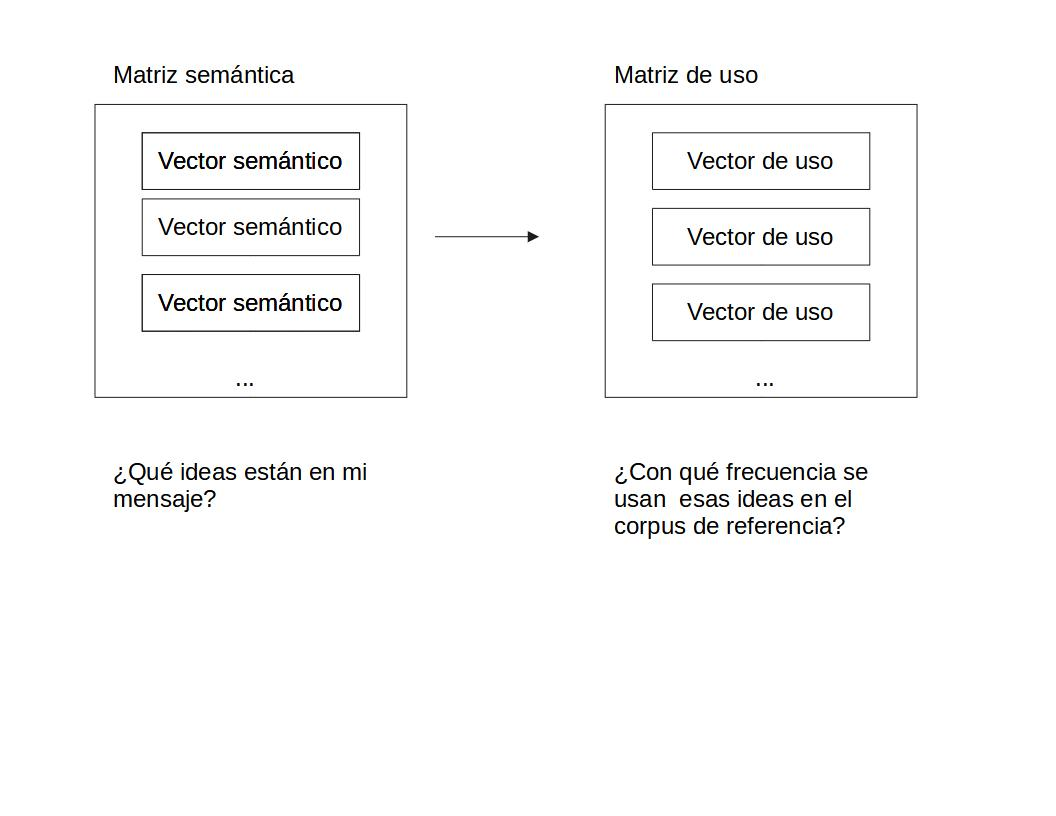
\includegraphics[width=0.7\textwidth]{./assets/matrices.jpg}
\caption{\label{fig:matrices}Transformación de matriz semántica a matríz de uso}
\end{figure}


\begin{figure}[H]
\centering
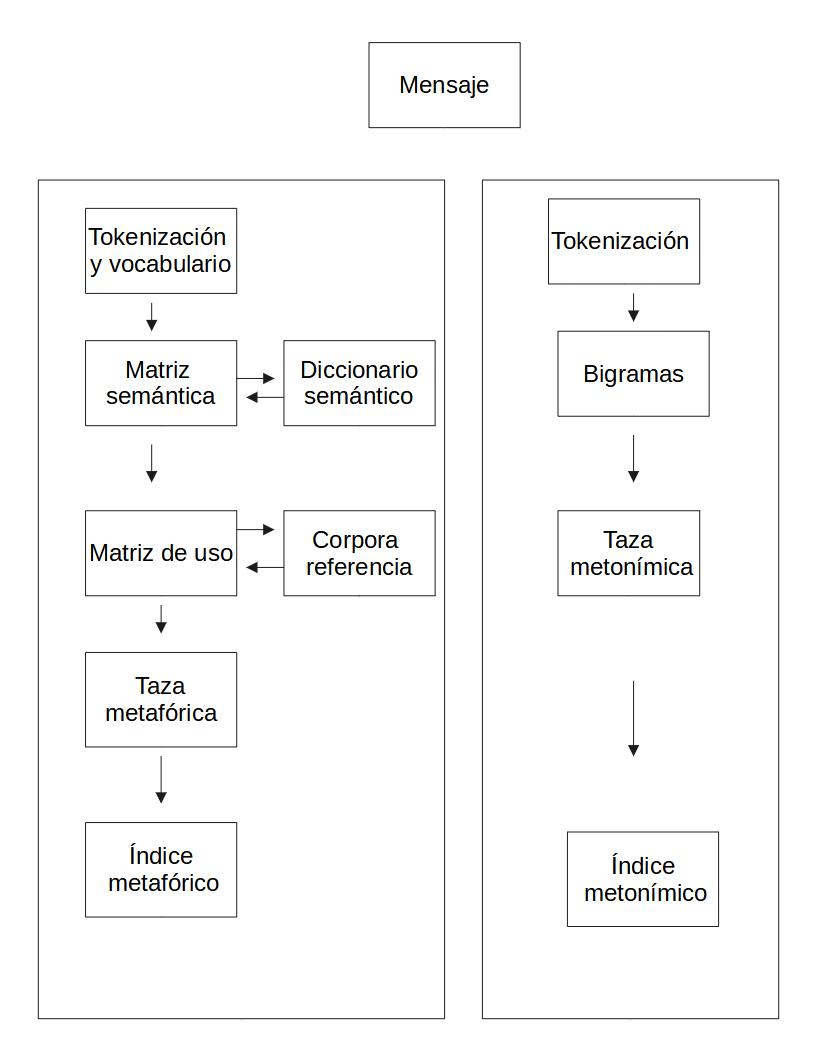
\includegraphics[width=0.7\textwidth]{./assets/metodologia.jpg}
\caption{\label{fig:metodologia}Etapas de procesamiento para cada índice}
\end{figure}

\begin{figure}[H]
\centering
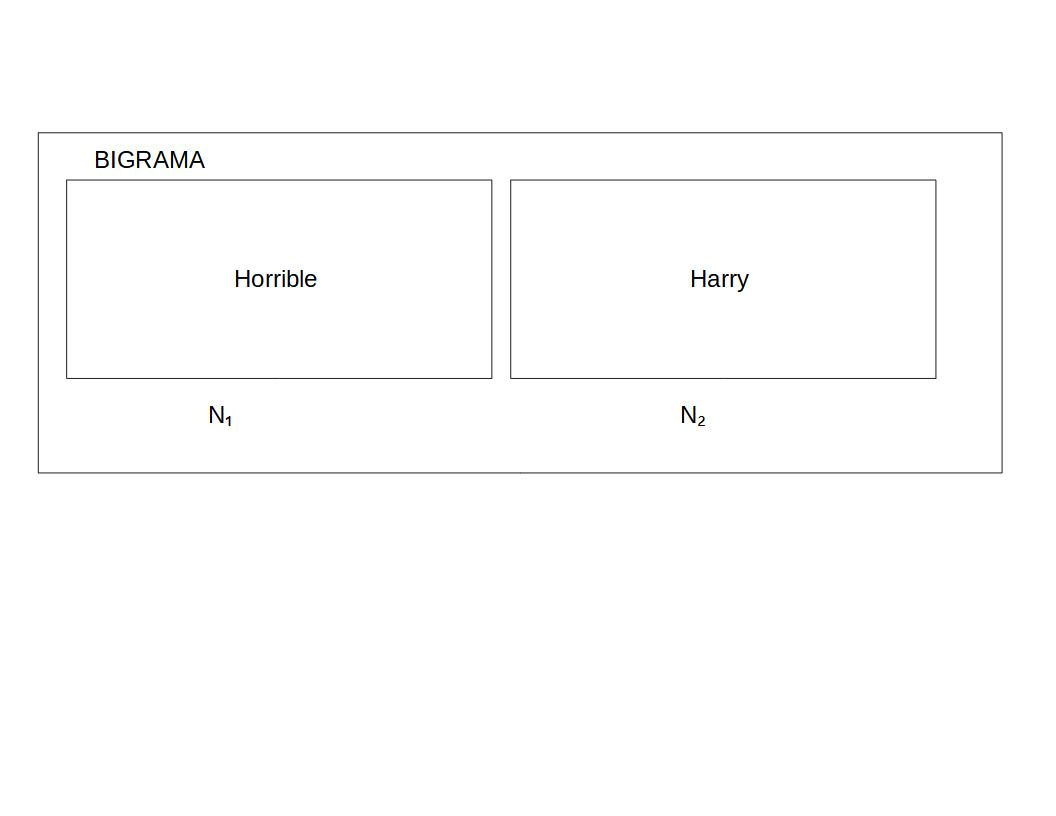
\includegraphics[width=0.7\textwidth]{./assets/metonimia.jpg}
\caption{\label{fig:metonimia}Concepto de metonimia}
\end{figure}

\subsection{Despliegue}
\label{sec:org1e226d2}
En las secciones \ref{sec:org390998b}, \ref{sec:org66a5e7c} y
\ref{sec:org0e8024f} se presentarán los resultados del experimento
según los parámetros descritos en las secciones anteriores.
La presentación va en creciente órden de abstracción, partiendo
de los datos brutos, pasando por su visualización, hasta llegar
a las Conclusiones .

\subsubsection{Índices por muestra}
\label{sec:org390998b}
En esta sección, se muestran los resultados producidos por el modelo
para cada uno de los corpus objetivos definidos en la sección
\ref{sec:org8537132}. En cada tabla se presentan el índice
metafórico y el índice metonímico para el representante de cada
categoría en las columnas 'metafora' y 'metonimia',
respectivamente. La columna 'w' simplemente representa el número de
palabras totales en el texto procesado, en caso de que en un futuro se
desee hacer comparaciones entre textos de diferentes tamaños.

Estos valores no tienen ningún tipo de procesamiento y para apreciarlos, es mejor
consultar las secciones \ref{sec:org66a5e7c} y \ref{sec:org0e8024f}.

\small
\begin{center}
    \begin{longtable}{| p{.20\textwidth} | p{.25\textwidth} | p{.25\textwidth}|p{.10\textwidth}|}
    \caption{Muestra 1}
    \hline
        categoria & metafora & metonimia & w \\ \hline
        reportage & 880514.226605173 & 232.266917233093 & 2340 \\ \hline
        editorial & 880324.393897166 & 245.719531857031 & 2262 \\ \hline
        reviews & 929802.38416219 & 242.953762332438 & 2370 \\ \hline
        religion & 850127.6846531 & 264.683072130827 & 2314 \\ \hline
        skills \& hobbies & 831781.725628903 & 242.632252469752 & 2232 \\ \hline
        popular lore & 833825.825225262 & 265.83988095238 & 2222 \\ \hline
        belles lettres & 877690.52541314 & 229.785869685869 & 2288 \\ \hline
        miscellaneous & 782613.273615479 & 278.192915417915 & 2214 \\ \hline
        learned & 863208.047211933 & 266.998263827676 & 2254 \\ \hline
        general fiction & 891211.57527208 & 249.95016095016 & 2264 \\ \hline
        mistery and detective fiction & 1032943.85669407 & 244.615023865023 & 2446 \\ \hline
        science fiction & 1064426.54657215 & 235.067805233981 & 2412 \\ \hline
        adventure and western fiction & 1234204.19460692 & 229.817769158945 & 2560 \\ \hline
        romance and love story & 993413.094671098 & 217.506968031968 & 2428 \\ \hline
\end{longtable}
\label{muestra1}
\end{center}

\begin{center}
    \begin{longtable}{| p{.20\textwidth} | p{.25\textwidth} | p{.25\textwidth}|p{.10\textwidth}|}
\caption{Muestra 2} 
    \hline
         categoria & metafora & metonimia & w \\ \hline
        reportage & 869205.2371696023 & 233.99592490842463 & 2277 \\ \hline
        editorial & 777241.5394134748 & 252.29809496059465 & 2200 \\ \hline
        reviews & 978095.225396233 & 242.3226565101564 & 2415 \\ \hline
        religion & 831466.3628116096 & 234.21091131091077 & 2213 \\ \hline
        skills \& hobbies & 833209.3790445685 & 237.43338605838585 & 2279 \\ \hline
        popular lore & 965391.1906183016 & 270.5444999444997 & 2369 \\ \hline
        belles lettres & 863139.7507327744 & 279.74454989454966 & 2289 \\ \hline
        miscellaneous & 873426.7117151126 & 302.2738428238428 & 2416 \\ \hline
        learned & 912477.0323082526 & 241.59998334998312 & 2189 \\ \hline
        general fiction & 1025249.8452137534 & 243.0625180375174 & 2440 \\ \hline
        mistery and detective fiction & 959584.2017381956 & 231.74134476634435 & 2370 \\ \hline
        science fiction & 1049847.7175834612 & 260.93059440559404 & 2486 \\ \hline
        adventure and western fiction & 1079790.9124281127 & 232.90989288489175 & 2383 \\ \hline
        romance and love story & 969075.2121776282 & 261.1946331446324 & 2332 \\ \hline
    \end{longtable}
    \label{muestra2}
\end{center}


\begin{center}
        \begin{longtable}{| p{.2\textwidth} | p{.25\textwidth} | p{.25\textwidth}|p{.10\textwidth}|}
\caption{Muestra 3}
    \hline
          categoria & metafora & metonimia & w \\ \hline
        reportage & 832961.122494042 & 253.461402486402 & 2275 \\ \hline
        editorial & 798751.012651529 & 266.66209346209246 & 2234 \\ \hline
        reviews & 884194.0844699917 & 249.01867299367268 & 2320 \\ \hline
        religion & 831865.8440237658 & 266.0598665223664 & 2332 \\ \hline
        skills \& hobbies & 850383.4965037219 & 263.1010350760349 & 2257 \\ \hline
        popular lore & 869221.9181097293 & 245.8761655011648 & 2264 \\ \hline
        belles lettres & 871094.3935751553 & 275.37426046176046 & 2311 \\ \hline
        miscellaneous & 839155.9869742717 & 295.0817980222388 & 2360 \\ \hline
        learned & 781733.2618728676 & 246.0817654567651 & 2182 \\ \hline
        general fiction & 924678.68595826 & 258.49646187146146 & 2325 \\ \hline
        mistery and detective fiction & 1123420.1486319497 & 259.7061299811289 & 2428 \\ \hline
        science fiction & 935994.4646234306 & 248.55044955044897 & 2364 \\ \hline
        adventure and western fiction & 1032713.1638679344 & 250.64708347208267 & 2380 \\ \hline
        romance and love story & 997559.1771764176 & 251.74584582084492 & 2320 \\ \hline
\end{longtable}
    \label{muestra3}
\end{center}

\begin{center}
\begin{longtable}{| p{.20\textwidth} | p{.25\textwidth} | p{.25\textwidth}|p{.10\textwidth}|}
\caption{Muestra 4}
    \hline
        categoria & metafora & metonimia & w \\ \hline
        reportage & 739005.545665808 & 273.2918525918524 & 2217 \\ \hline
        editorial & 839392.6586708553 & 252.962795537795 & 2230 \\ \hline
        reviews & 897166.8448193009 & 267.3208680208676 & 2356 \\ \hline
        religion & 971902.397216239 & 265.22606282606193 & 2410 \\ \hline
        skills \& hobbies & 913636.3833983988 & 260.77830780330754 & 2295 \\ \hline
        popular lore & 827298.639753781 & 263.91099178599177 & 2256 \\ \hline
        belles lettres & 948168.5408124946 & 263.5388195138189 & 2403 \\ \hline
        miscellaneous & 863483.173212439 & 246.39977799977743 & 2207 \\ \hline
        learned & 842569.1577530246 & 231.37843986079253 & 2205 \\ \hline
        general fiction & 917557.8900258496 & 230.44950882450823 & 2296 \\ \hline
        mistery and detective fiction & 866731.5026959036 & 245.56009546009463 & 2288 \\ \hline
        science fiction & 1102841.6209263606 & 248.0798007548002 & 2461 \\ \hline
        adventure and western fiction & 976789.2077744814 & 253.20416527916453 & 2349 \\ \hline
        romance and love story & 1111028.8409040042 & 248.49708902208823 & 2422 \\ \hline


\end{longtable}
    \label{muestra4}
\end{center}

\begin{center}
\begin{longtable}{| p{.20\textwidth} | p{.25\textwidth} | p{.25\textwidth}|p{.10\textwidth}|}
\caption{Muestra 5}
    \hline
        categoria & metafora & metonimia & w \\ \hline
        reportage & 804307.8590497638 & 254.57564380064355 & 2244 \\ \hline
        editorial & 797847.982604727 & 256.40300255300195 & 2241 \\ \hline
        reviews & 926295.4083615864 & 234.46358363858295 & 2342 \\ \hline
        religion & 935931.8321572712 & 233.24144189144172 & 2317 \\ \hline
        skills \& hobbies & 916884.62774593 & 232.22511377511276 & 2370 \\ \hline
        popular lore & 796816.1152101667 & 263.7263361638353 & 2258 \\ \hline
        belles lettres & 861343.6692835388 & 239.3655889861766 & 2359 \\ \hline
        miscellaneous & 863173.038736266 & 279.4144463379755 & 2316 \\ \hline
        learned & 907069.3580927892 & 255.3453282828281 & 2334 \\ \hline
        general fiction & 870179.8901159727 & 224.0298867798861 & 2345 \\ \hline
        mistery and detective fiction & 914219.7991227966 & 256.1841630591622 & 2331 \\ \hline
        science fiction & 1000556.046812526 & 255.7852647352645 & 2369 \\ \hline
        adventure and western fiction & 835693.3281863902 & 228.3971750471748 & 2279 \\ \hline
        romance and love story & 1113220.902539808 & 261.2546370296359 & 2546 \\ \hline
\end{longtable}
    \label{muestra5}
\end{center}

\normalsize
\subsubsection{Gráficos por muestra}
\label{sec:org66a5e7c}
En esta sección se presentan los gráficos para cada uno de los corpus objetivos
definidos en \ref{sec:org8537132}. Cada cúmulo de gráficos consta de 2 filas.
La primera fila muestra el puntaje para el \textbf{índice metafórico} (izquierda) y
el \textbf{índice metonímico} (derecha) a través de las categorías, como están
definidas en el corpus de Brown. Por otro lado, en la segunda fila
se presentan los mismos puntajes para las metacategorías de de \textbf{ficción}
y \textbf{no ficción}. Las metacategorias son agrupaciones de categorías del corpus
de Brown y tienen el objetivo de evidenciar más claramente el comportamiento
de los dos índices de manera más general.

Para la producción de estos gráficos, se tomaron los resultados presentados en \ref{sec:org390998b}, y
se normalizaron con la técnica Min Max. En cada corpus objetivo, por lo tanto, se evidencia que
hay una categoría con el valor mínimo de 0 y otra con el valor máximo de 1. Esto evidencia
mejor la relación entre las distintas categorias en cuanto a las dos medidas postulados: la metáfora
y la metonimia.

\begin{figure}[H]
\centering
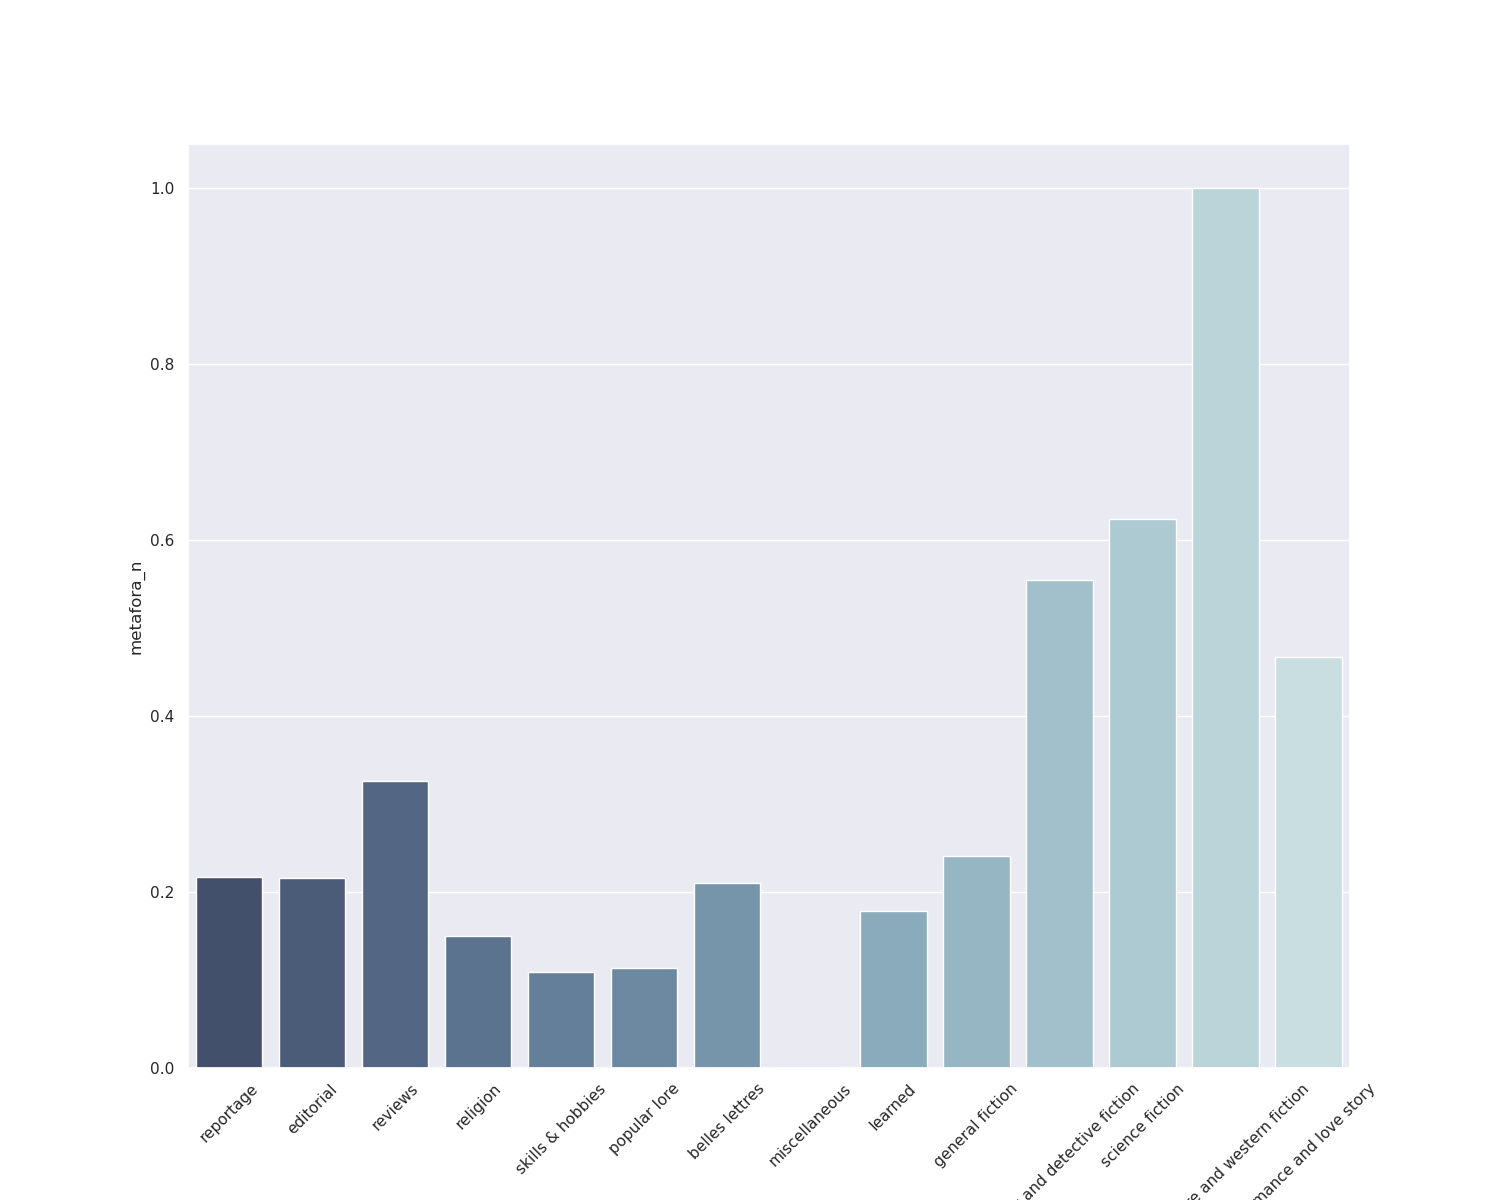
\includegraphics[width=.45\linewidth]{./resultados/graphs/muestra/c1_metafora.png}
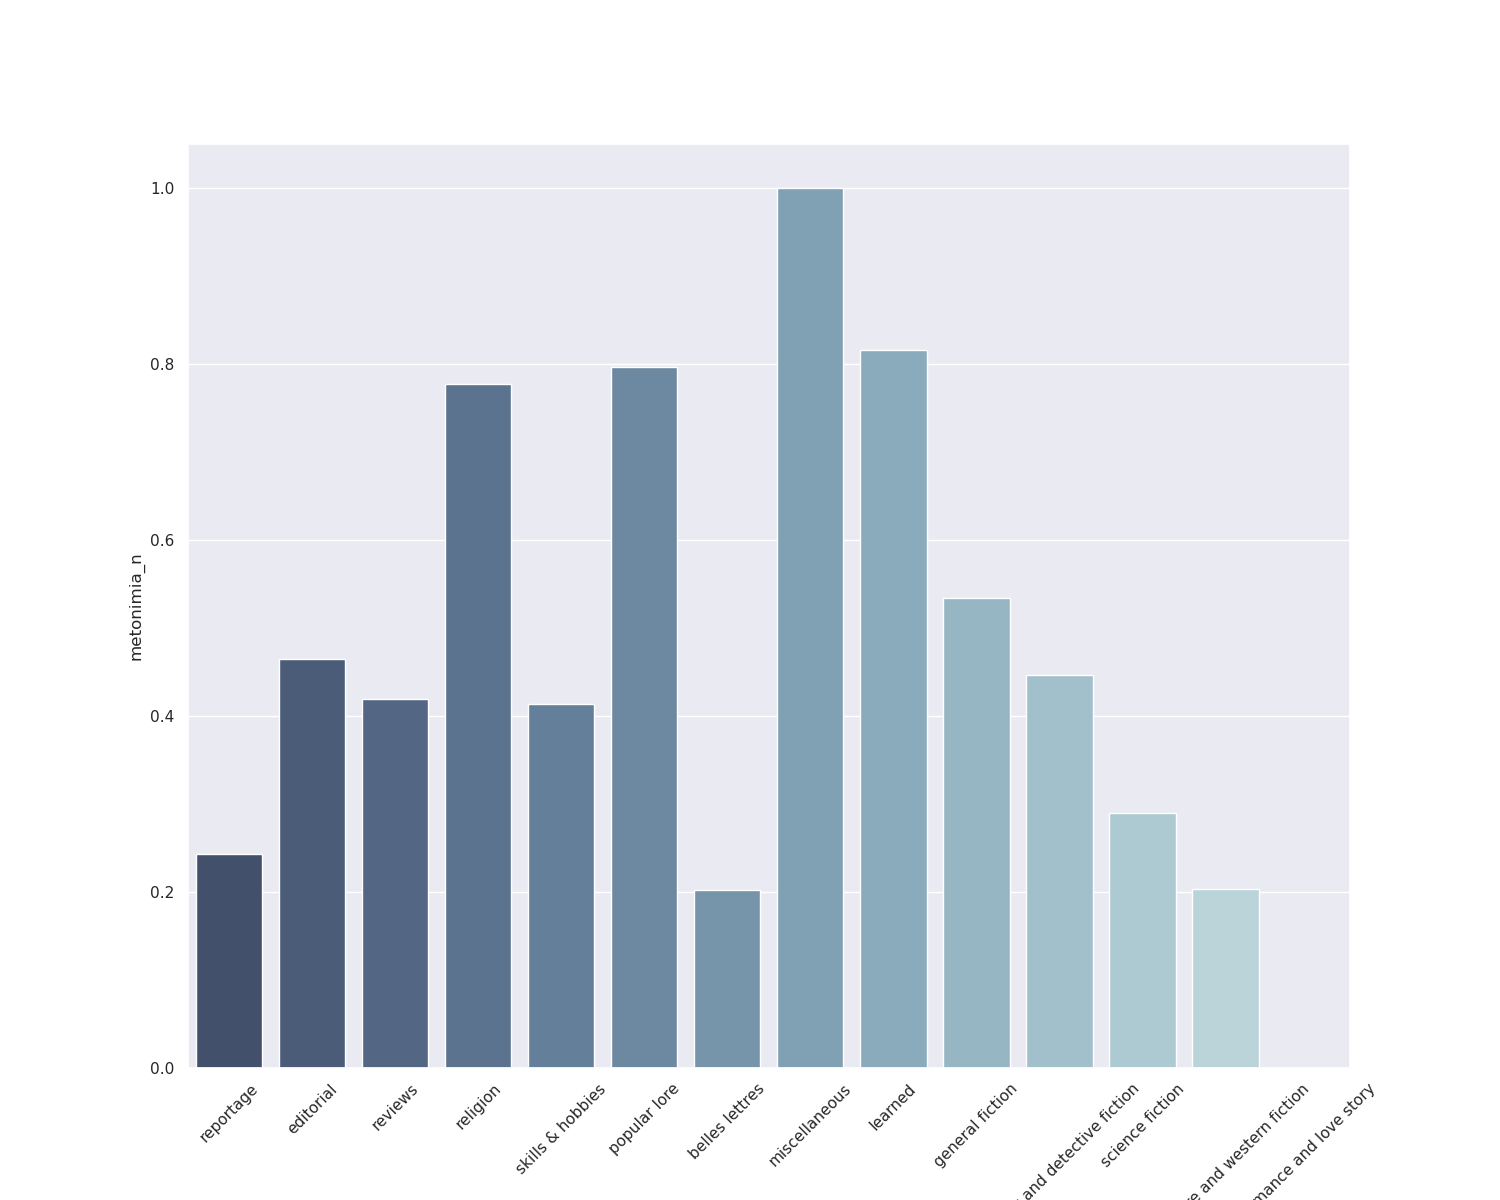
\includegraphics[width=.45\linewidth]{./resultados/graphs/muestra/c1_metonimia.png}
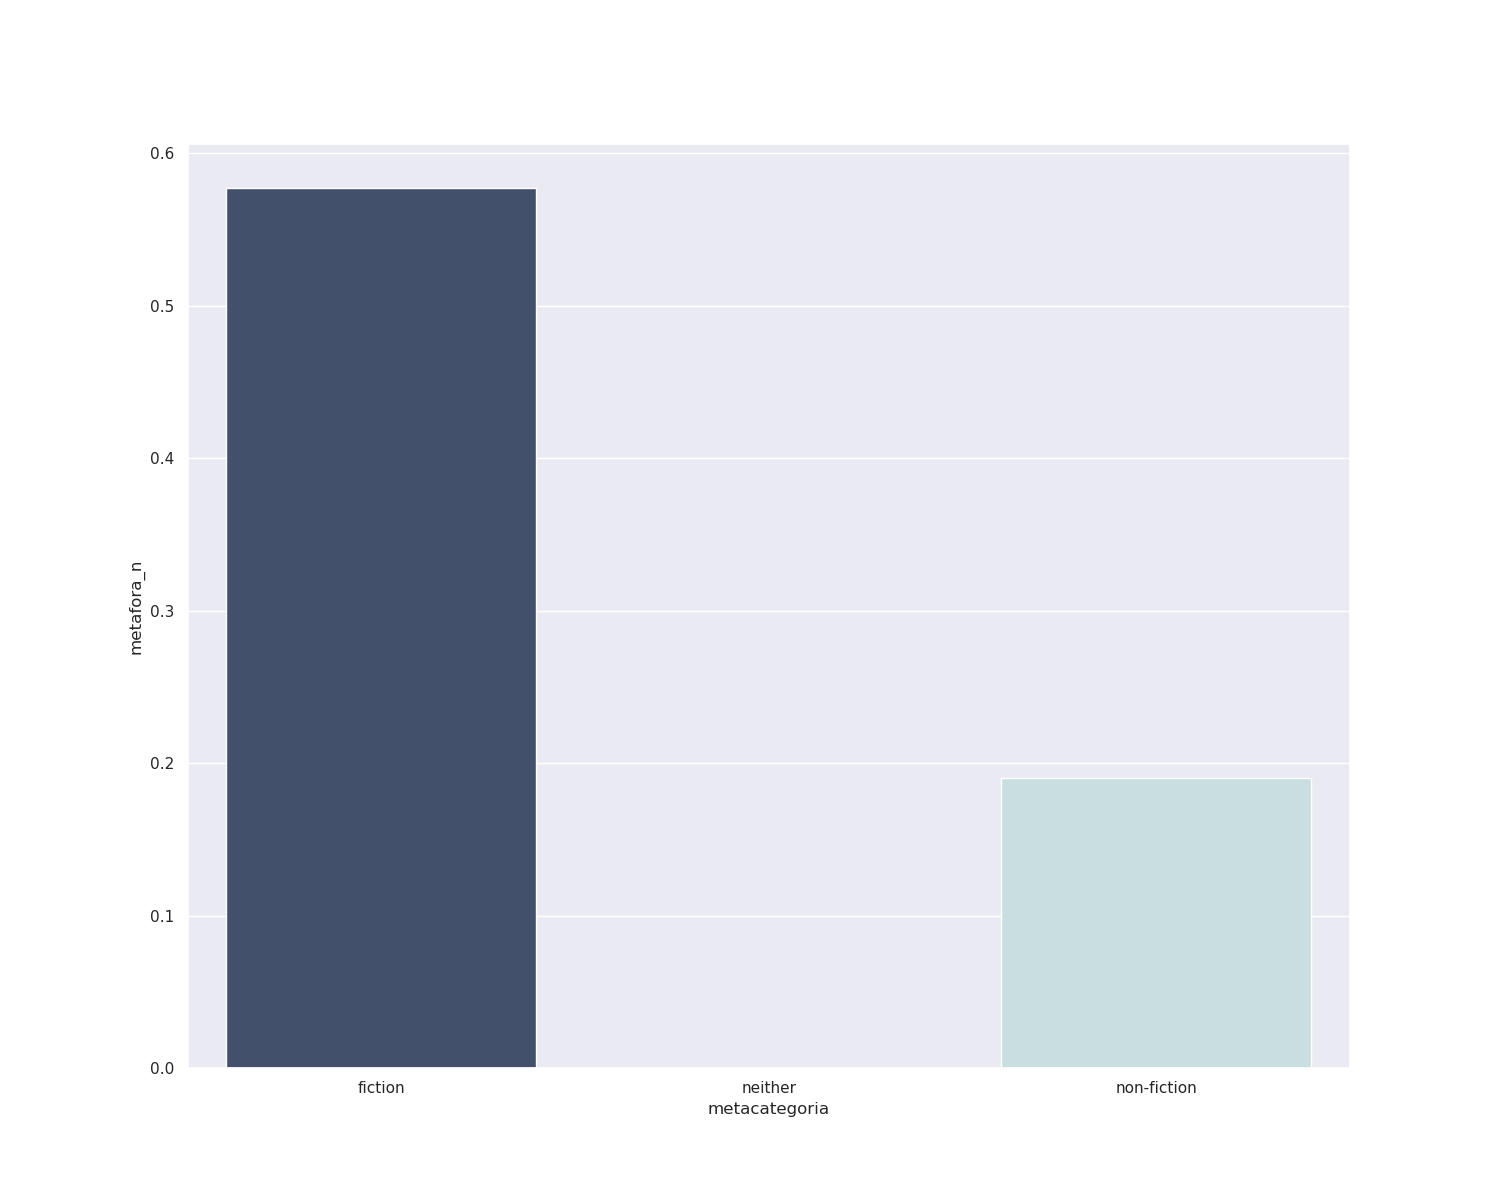
\includegraphics[width=.45\linewidth]{./resultados/graphs/meta/c1_metacategoria_metafora.png}
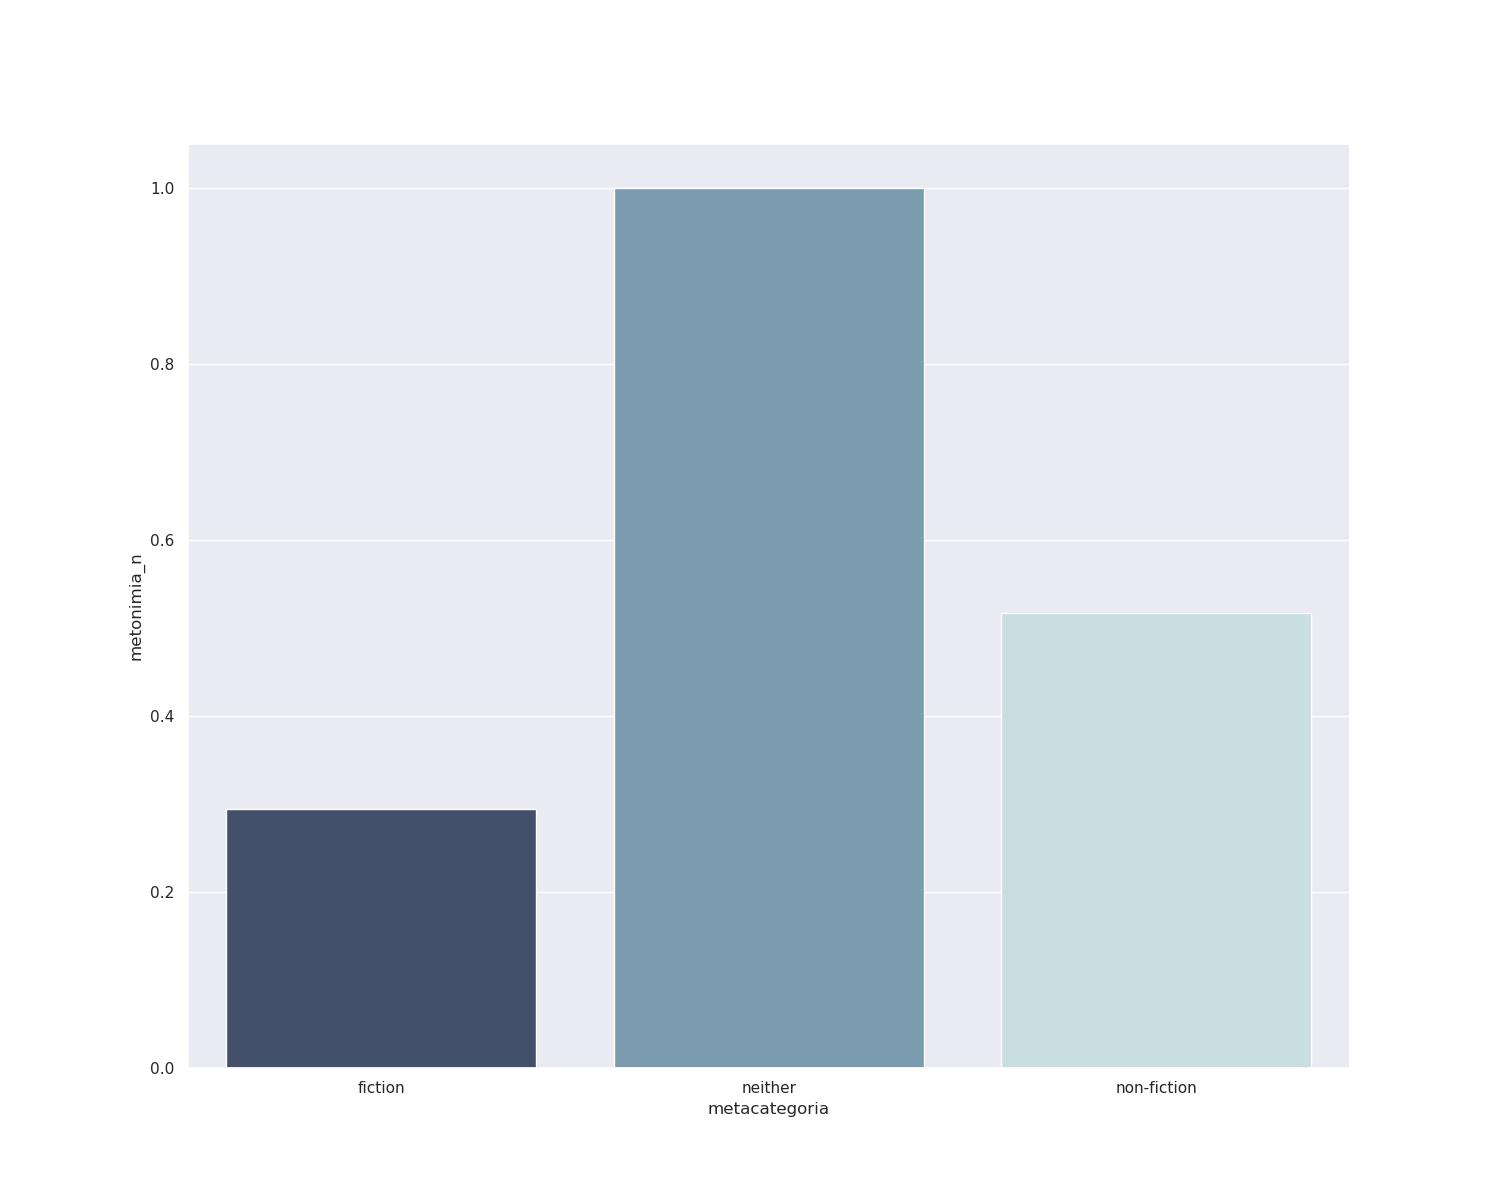
\includegraphics[width=.45\linewidth]{./resultados/graphs/meta/c1_metacategoria_metonimia.png}
\caption{\label{fig:c1_resultados}Resultados muestra 1}
\end{figure}


\begin{figure}[H]
\centering
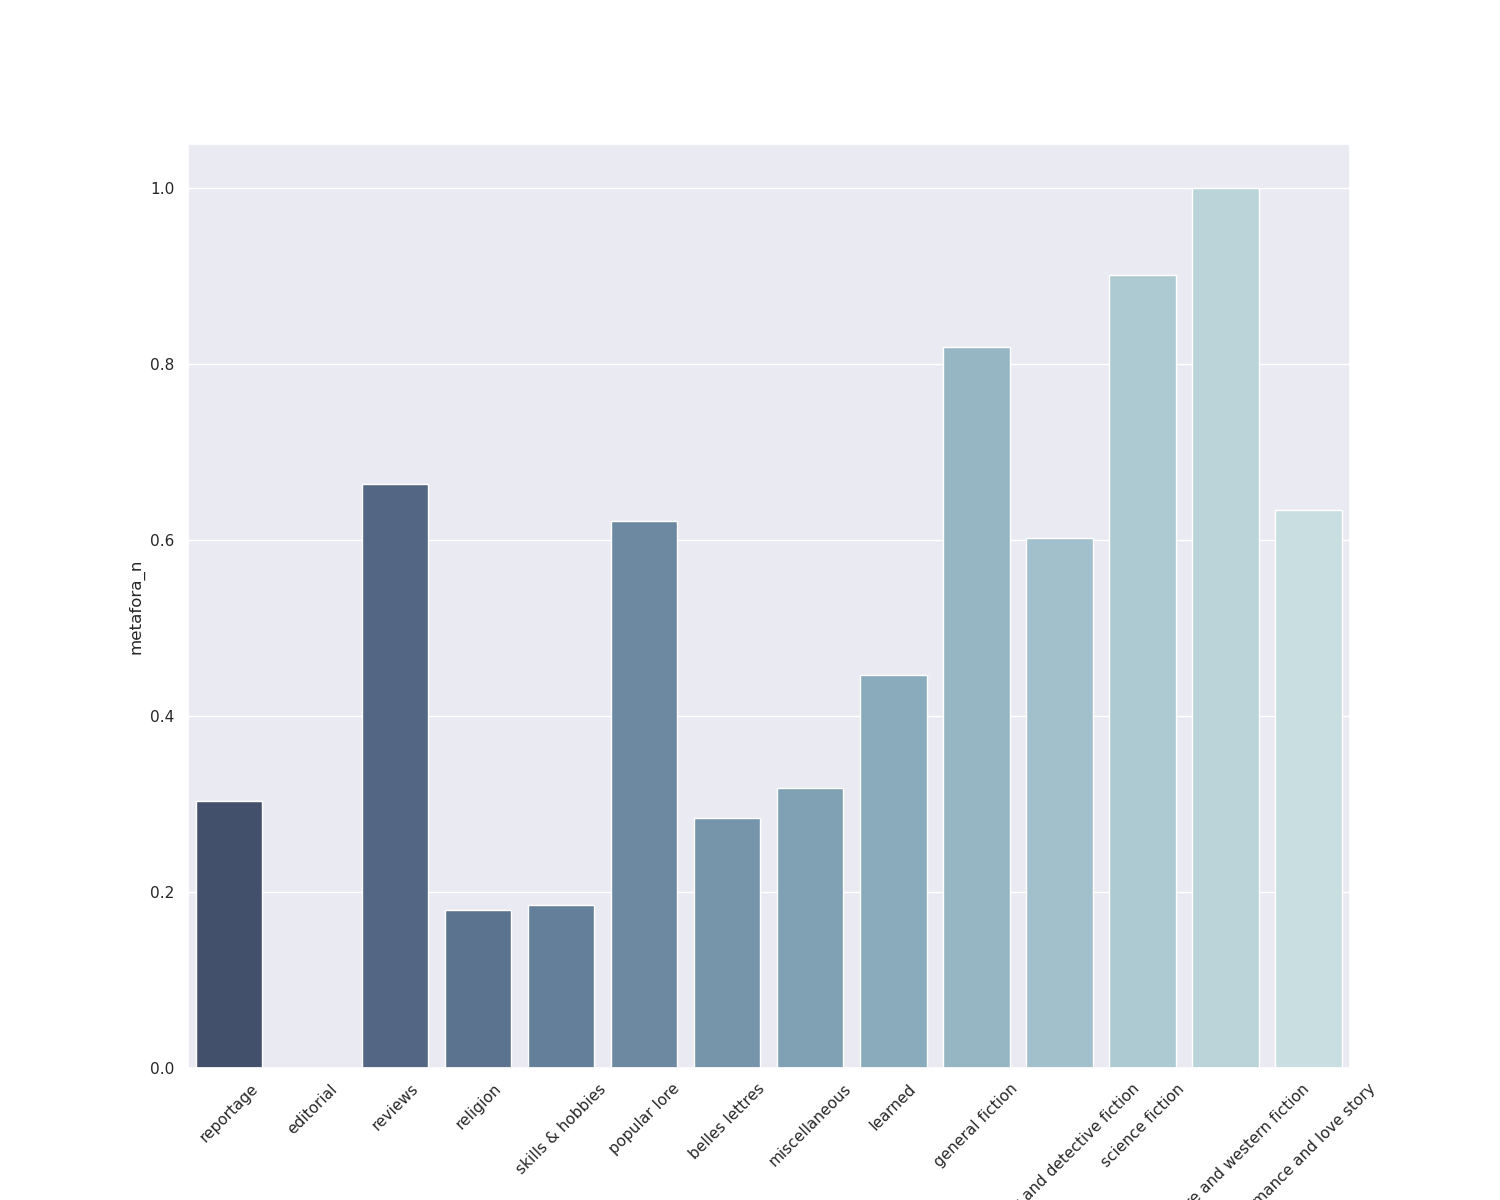
\includegraphics[width=.45\linewidth]{./resultados/graphs/muestra/c2_metafora.png}
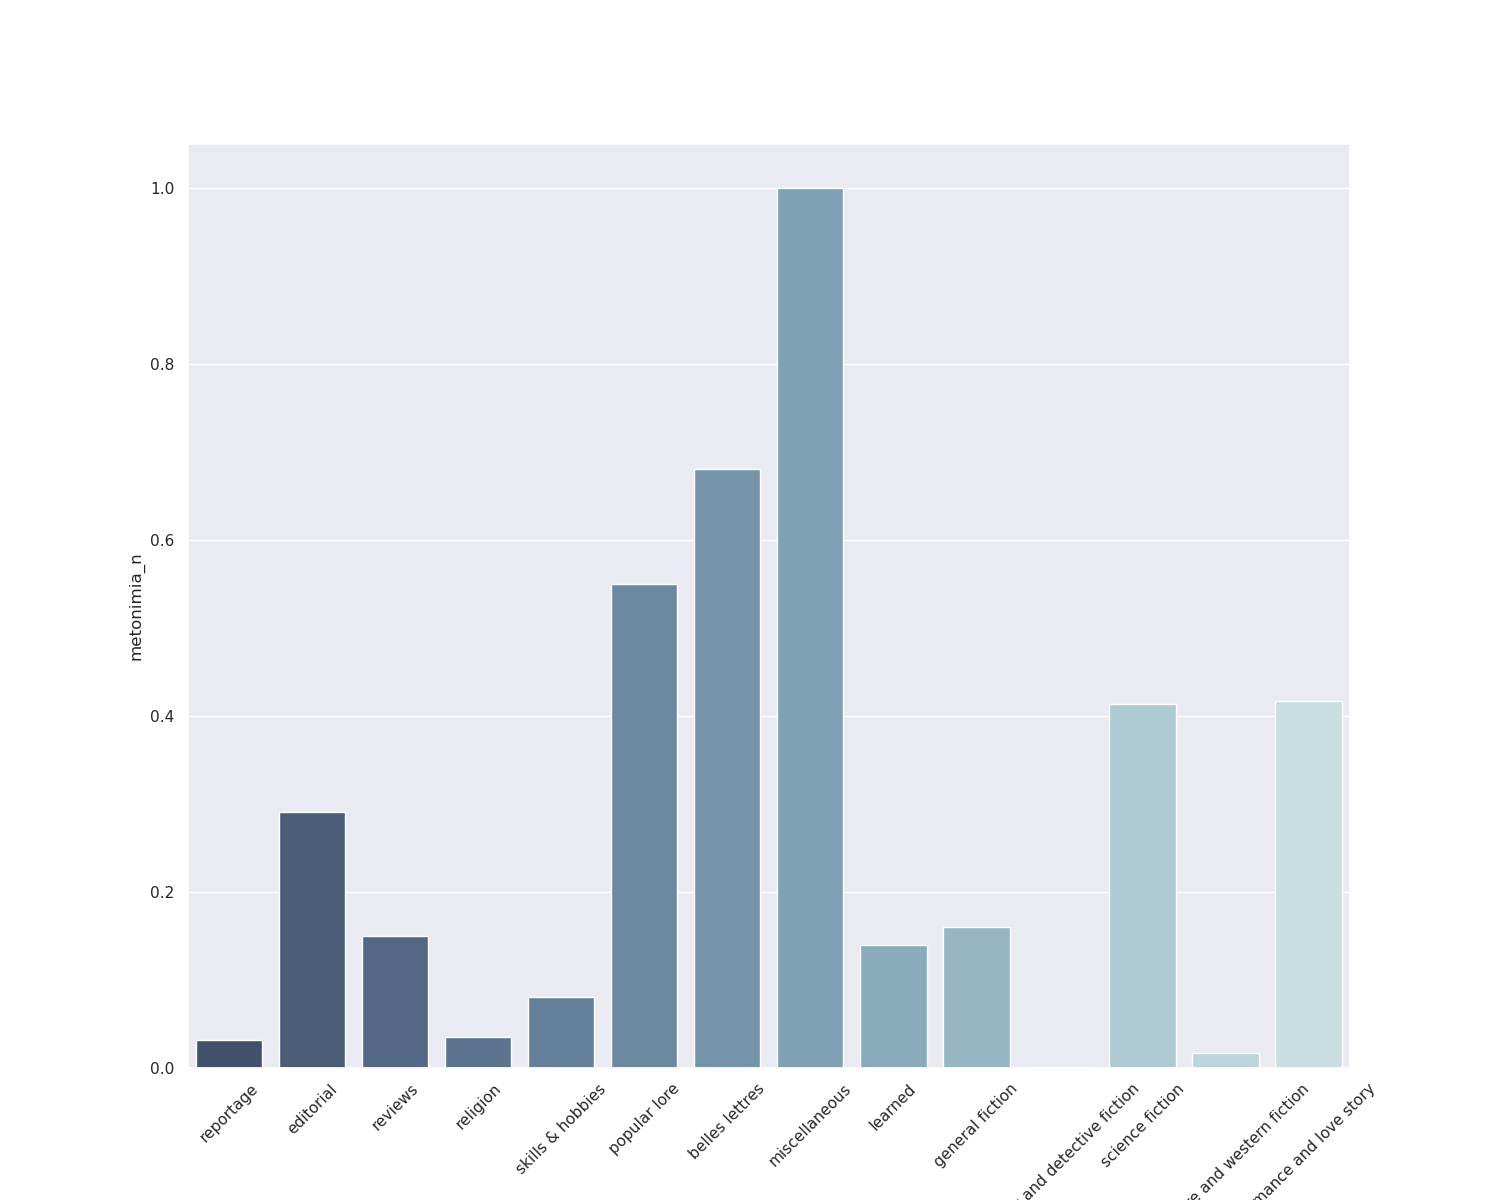
\includegraphics[width=.45\linewidth]{./resultados/graphs/muestra/c2_metonimia.png}
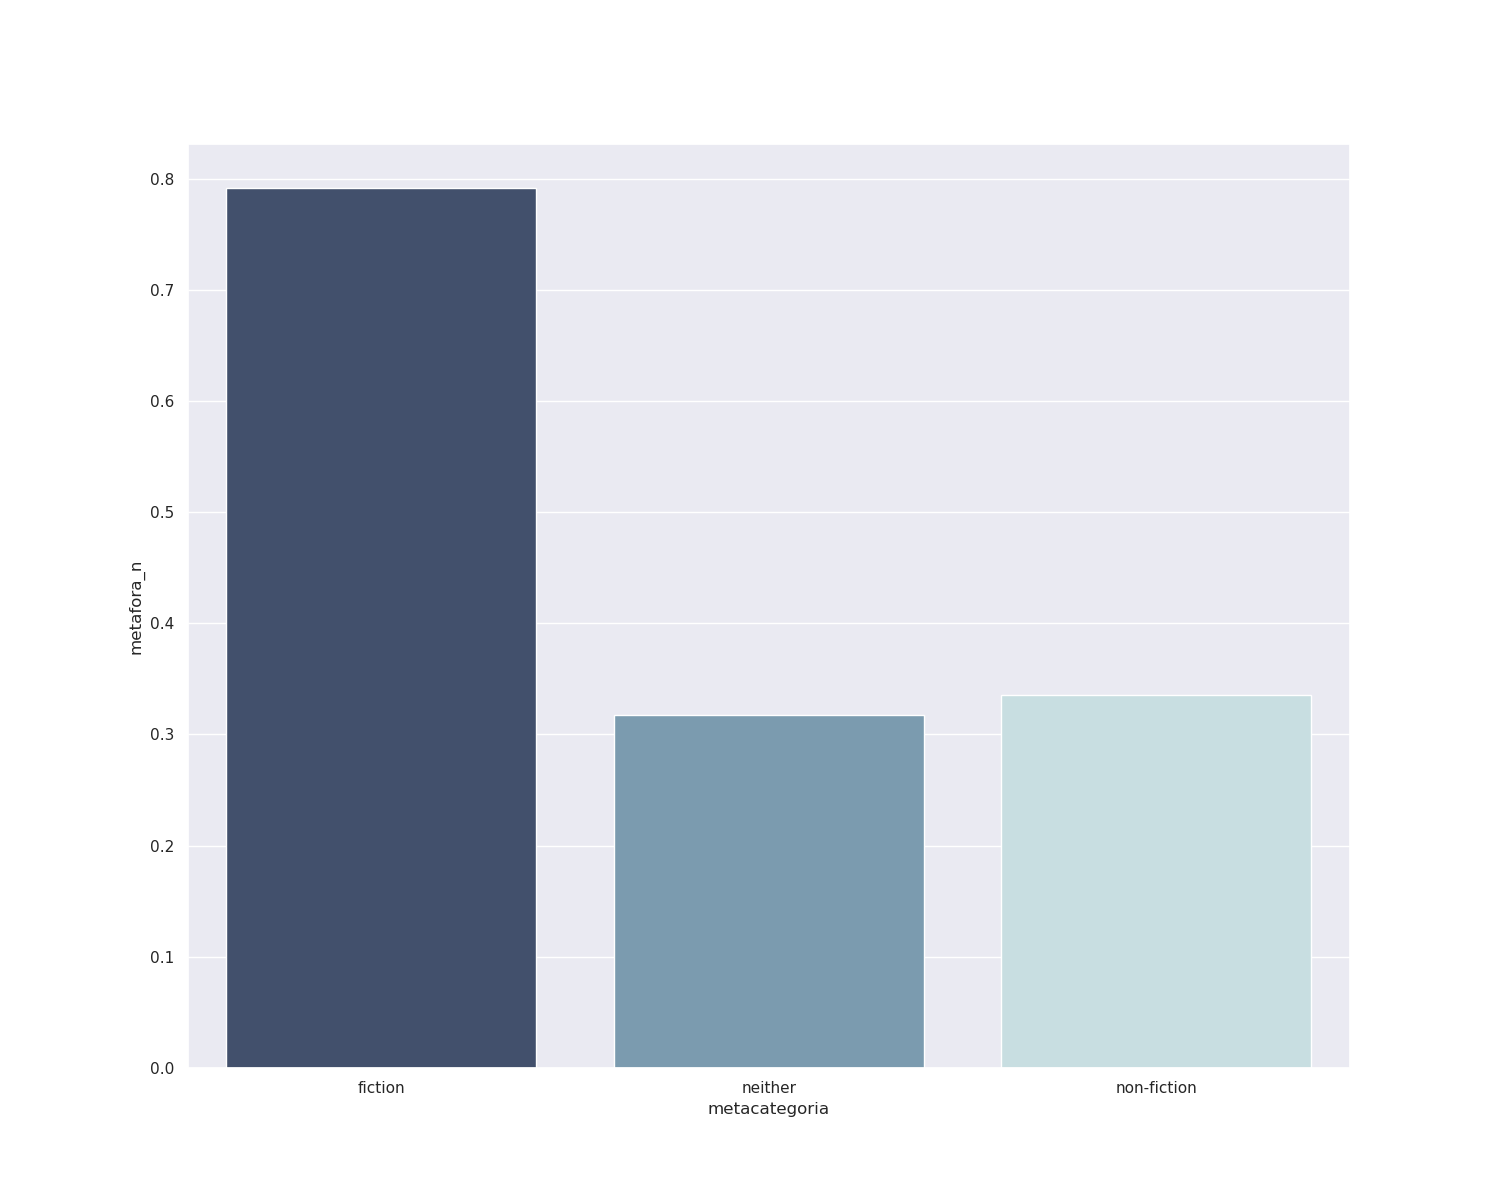
\includegraphics[width=.45\linewidth]{./resultados/graphs/meta/c2_metacategoria_metafora.png}
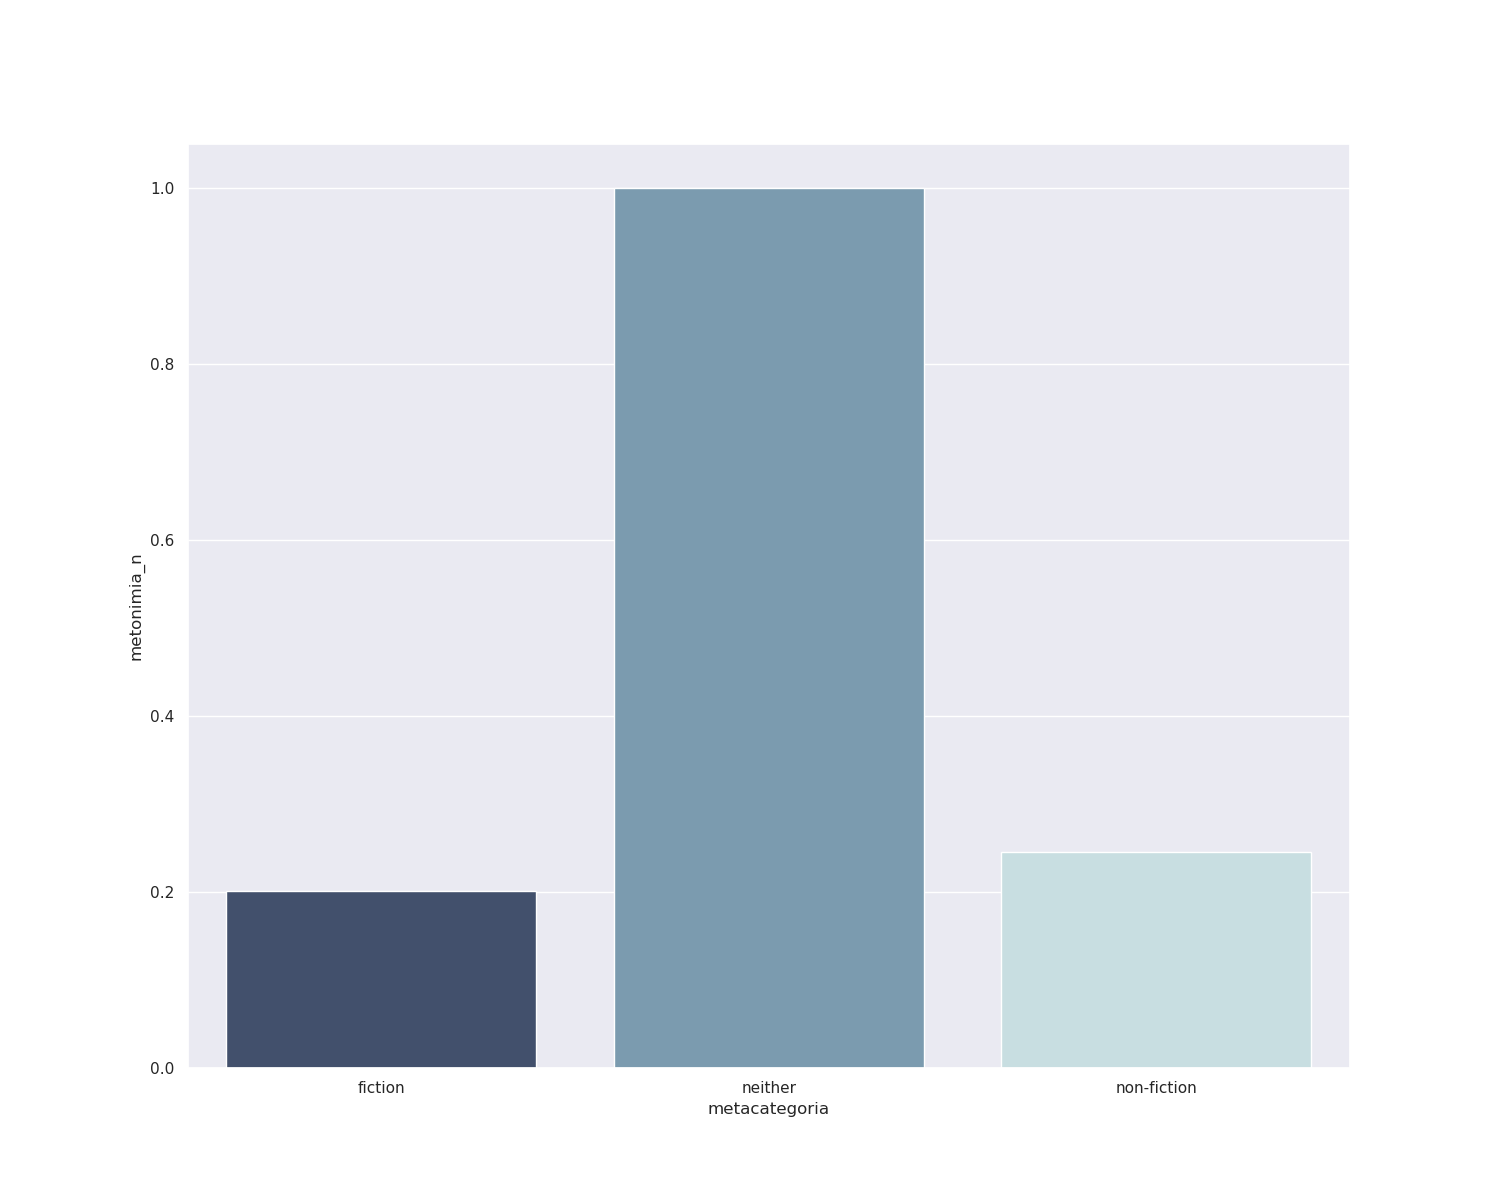
\includegraphics[width=.45\linewidth]{./resultados/graphs/meta/c2_metacategoria_metonimia.png}
\caption{\label{fig:c2_resultados}Resultados muestra 2}
\end{figure}

\begin{figure}[H]
\centering
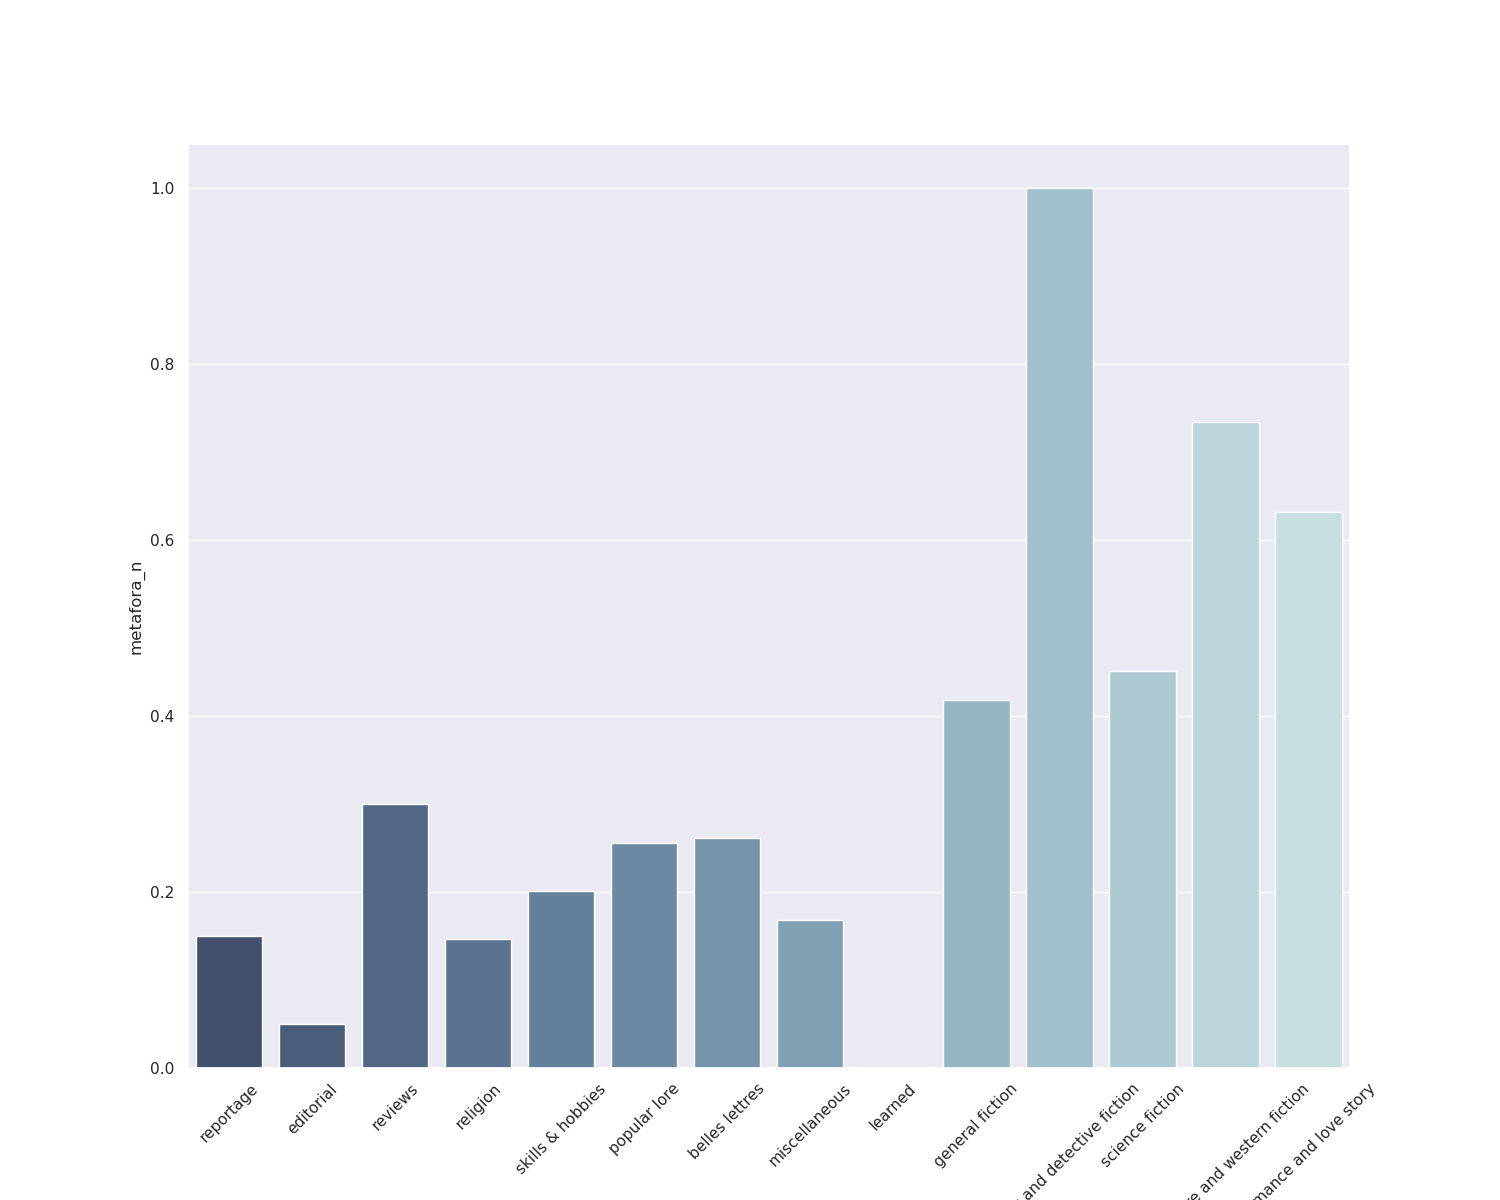
\includegraphics[width=.45\linewidth]{./resultados/graphs/muestra/c3_metafora.png}
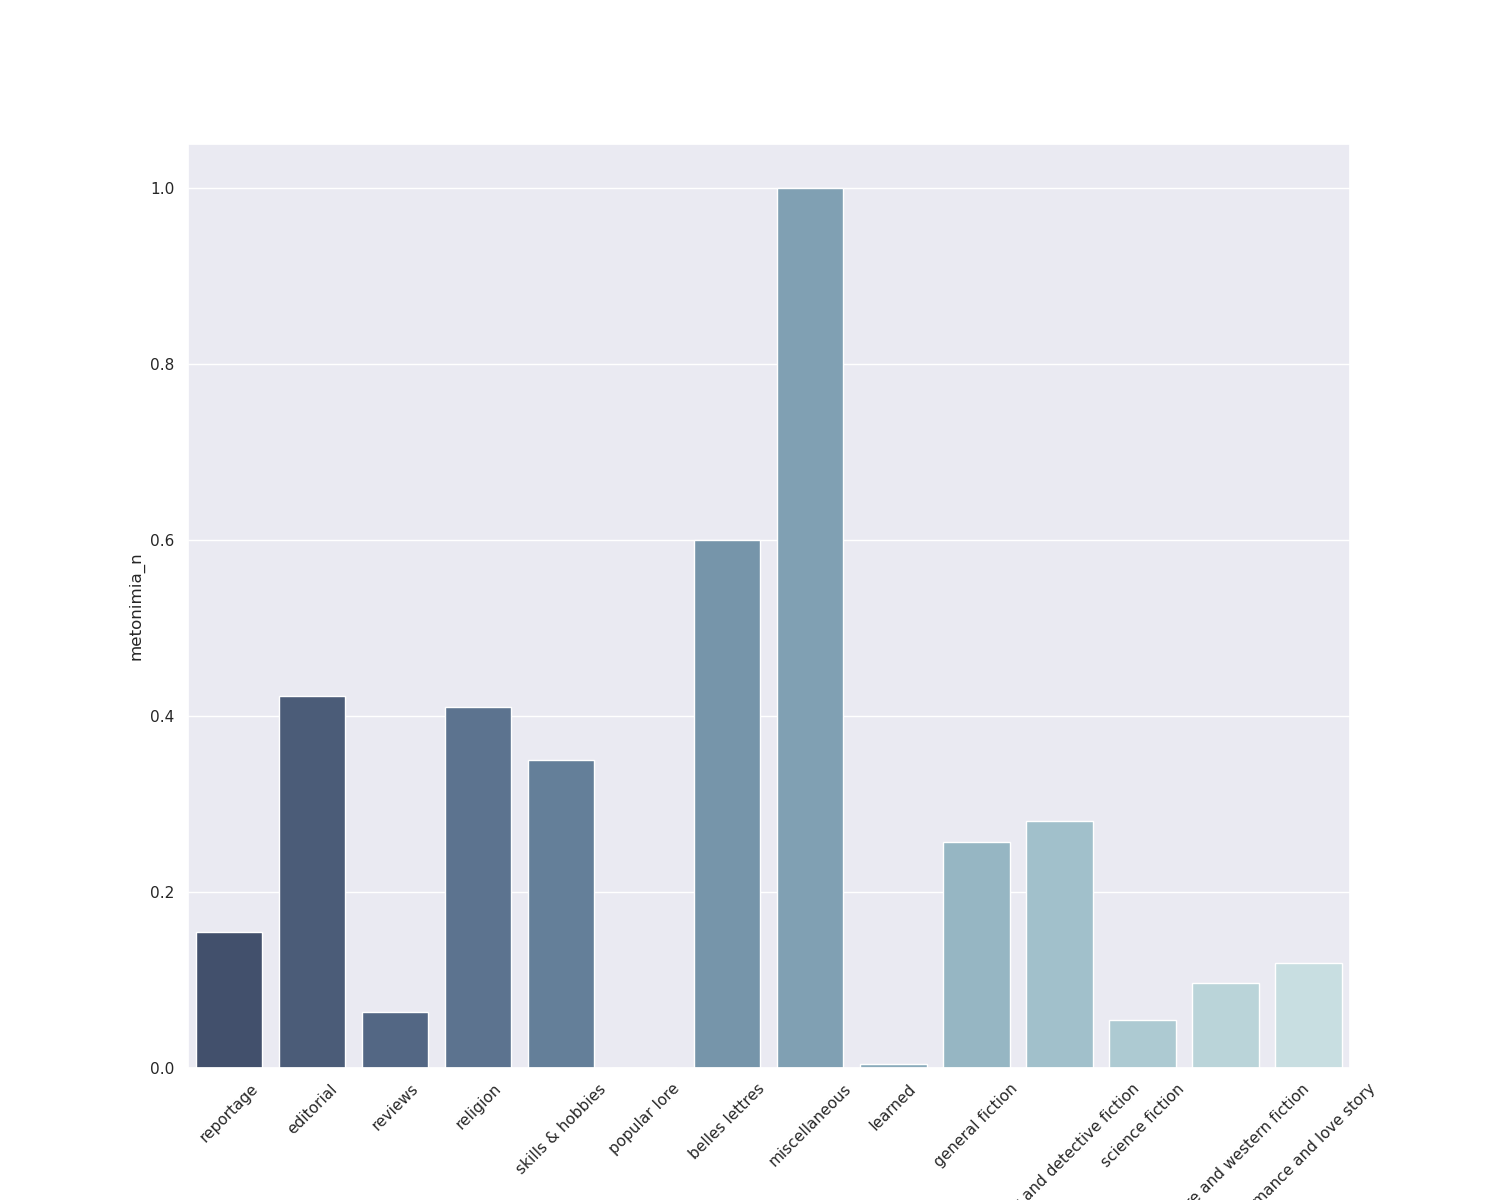
\includegraphics[width=.45\linewidth]{./resultados/graphs/muestra/c3_metonimia.png}
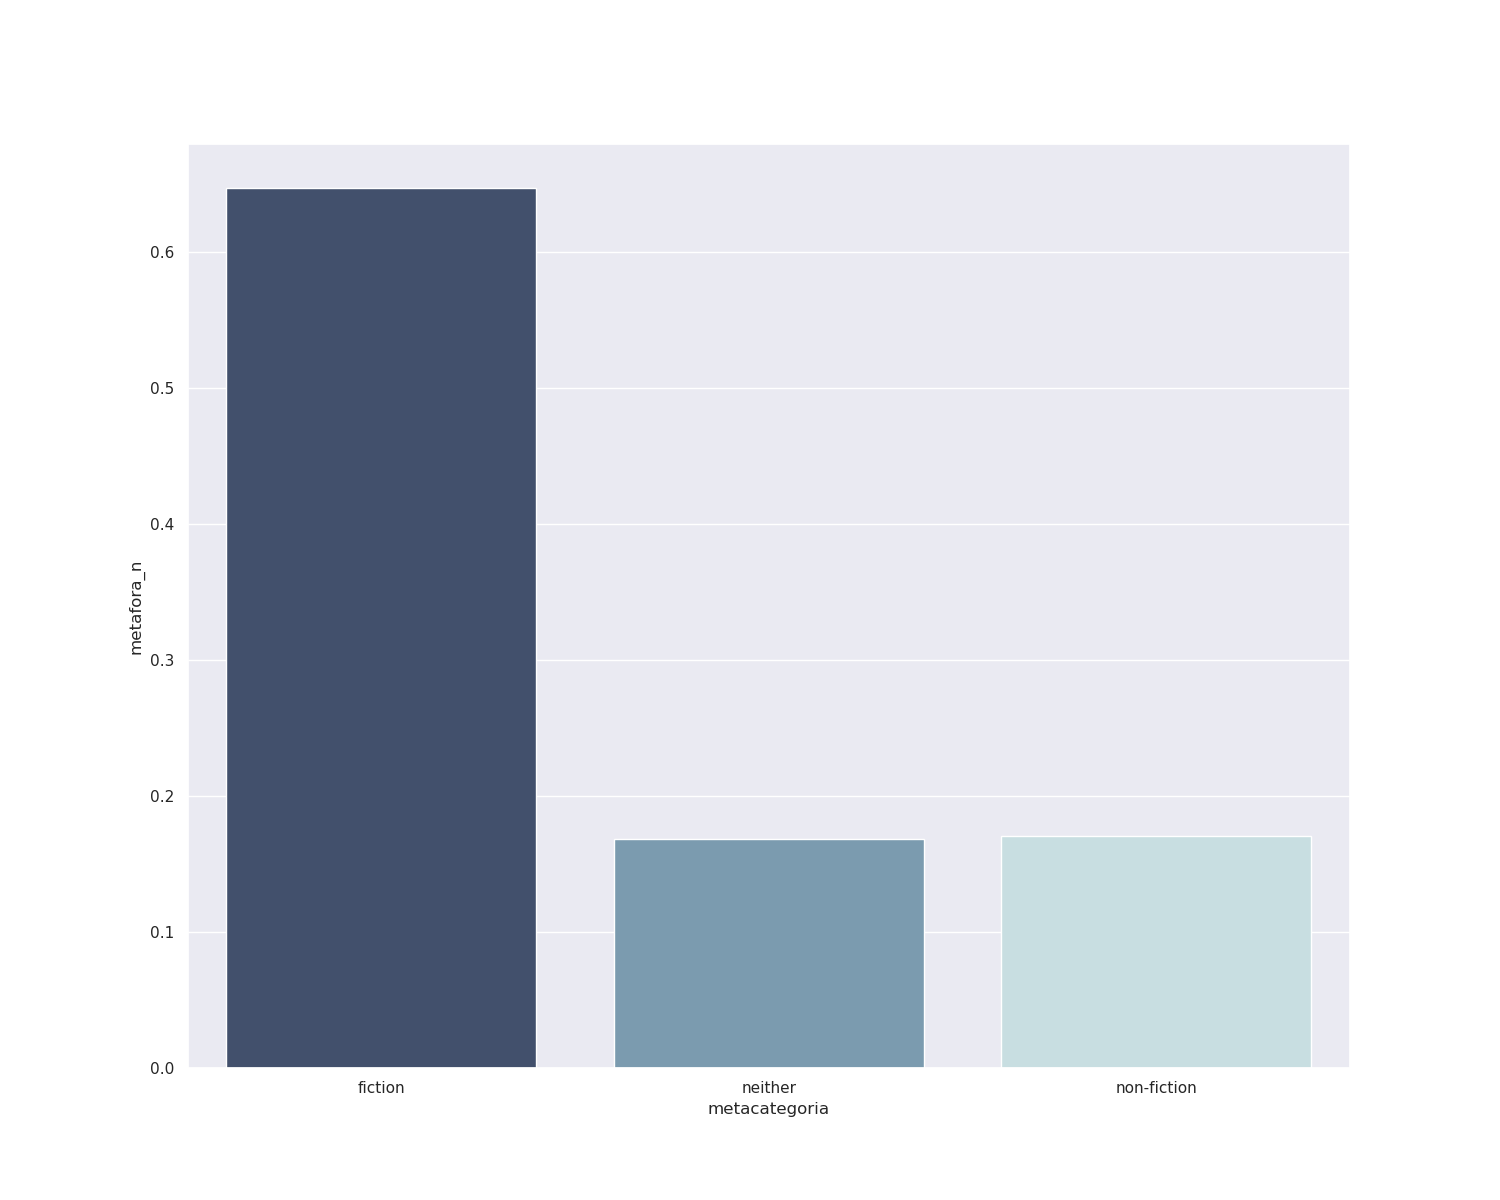
\includegraphics[width=.45\linewidth]{./resultados/graphs/meta/c3_metacategoria_metafora.png}
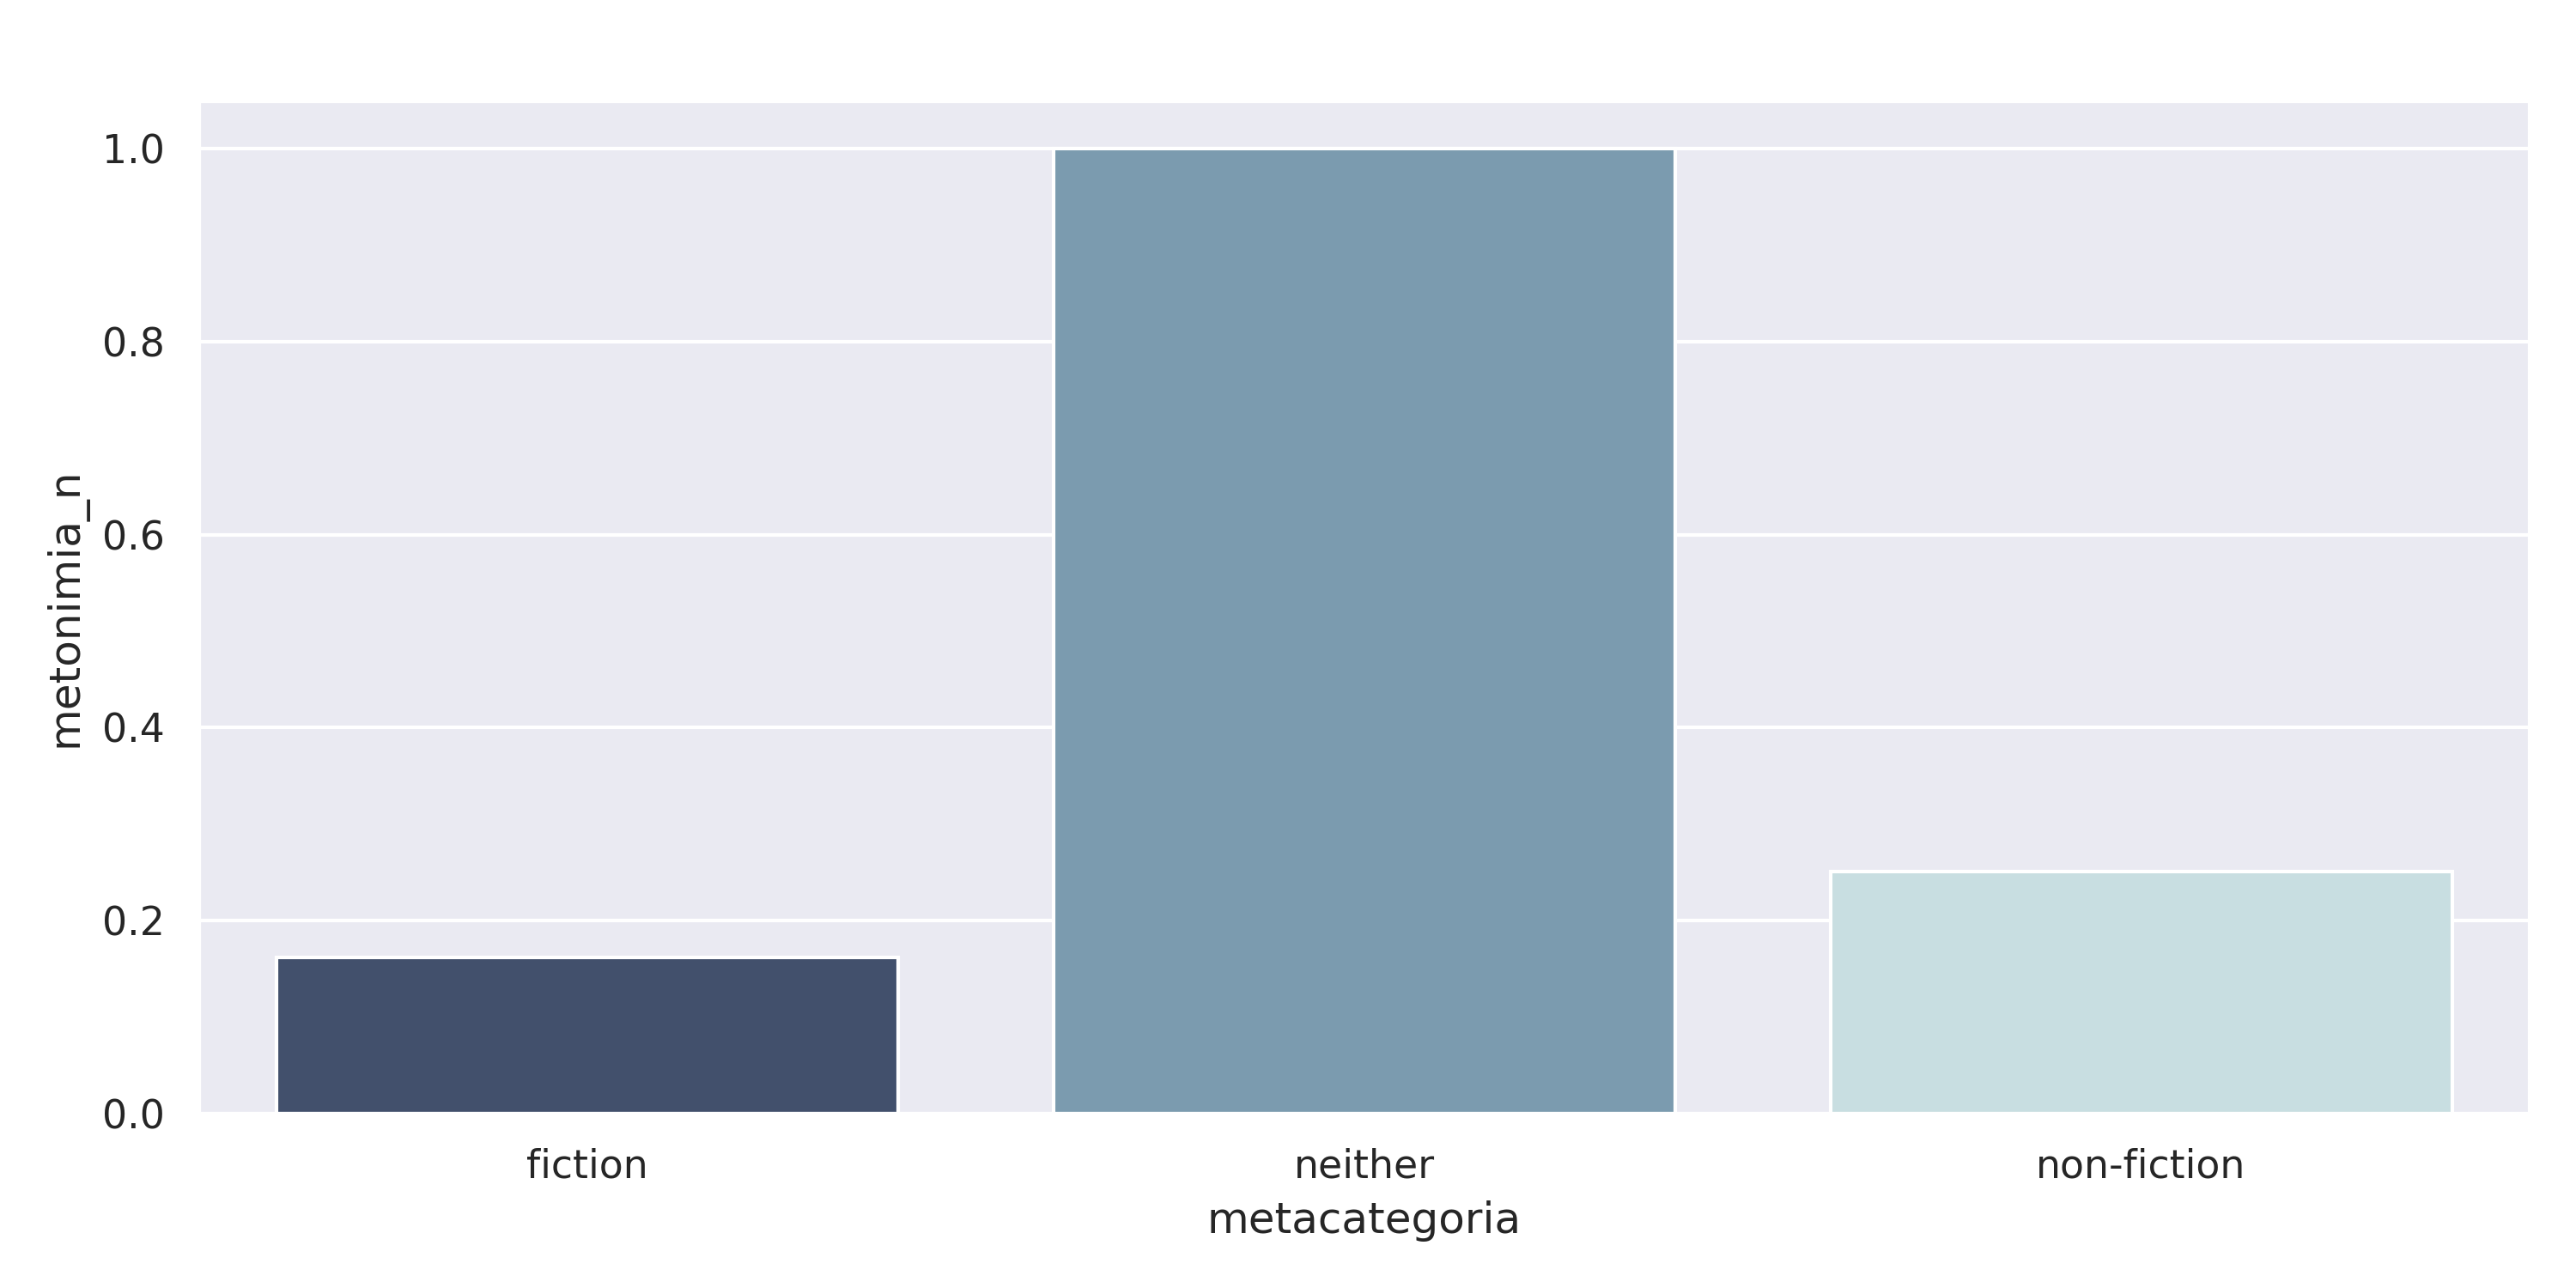
\includegraphics[width=.45\linewidth]{./resultados/graphs/meta/c3_metacategoria_metonimia.png}
\caption{\label{fig:c3_resultados}Resultados muestra 3}
\end{figure}

\begin{figure}[H]
\centering
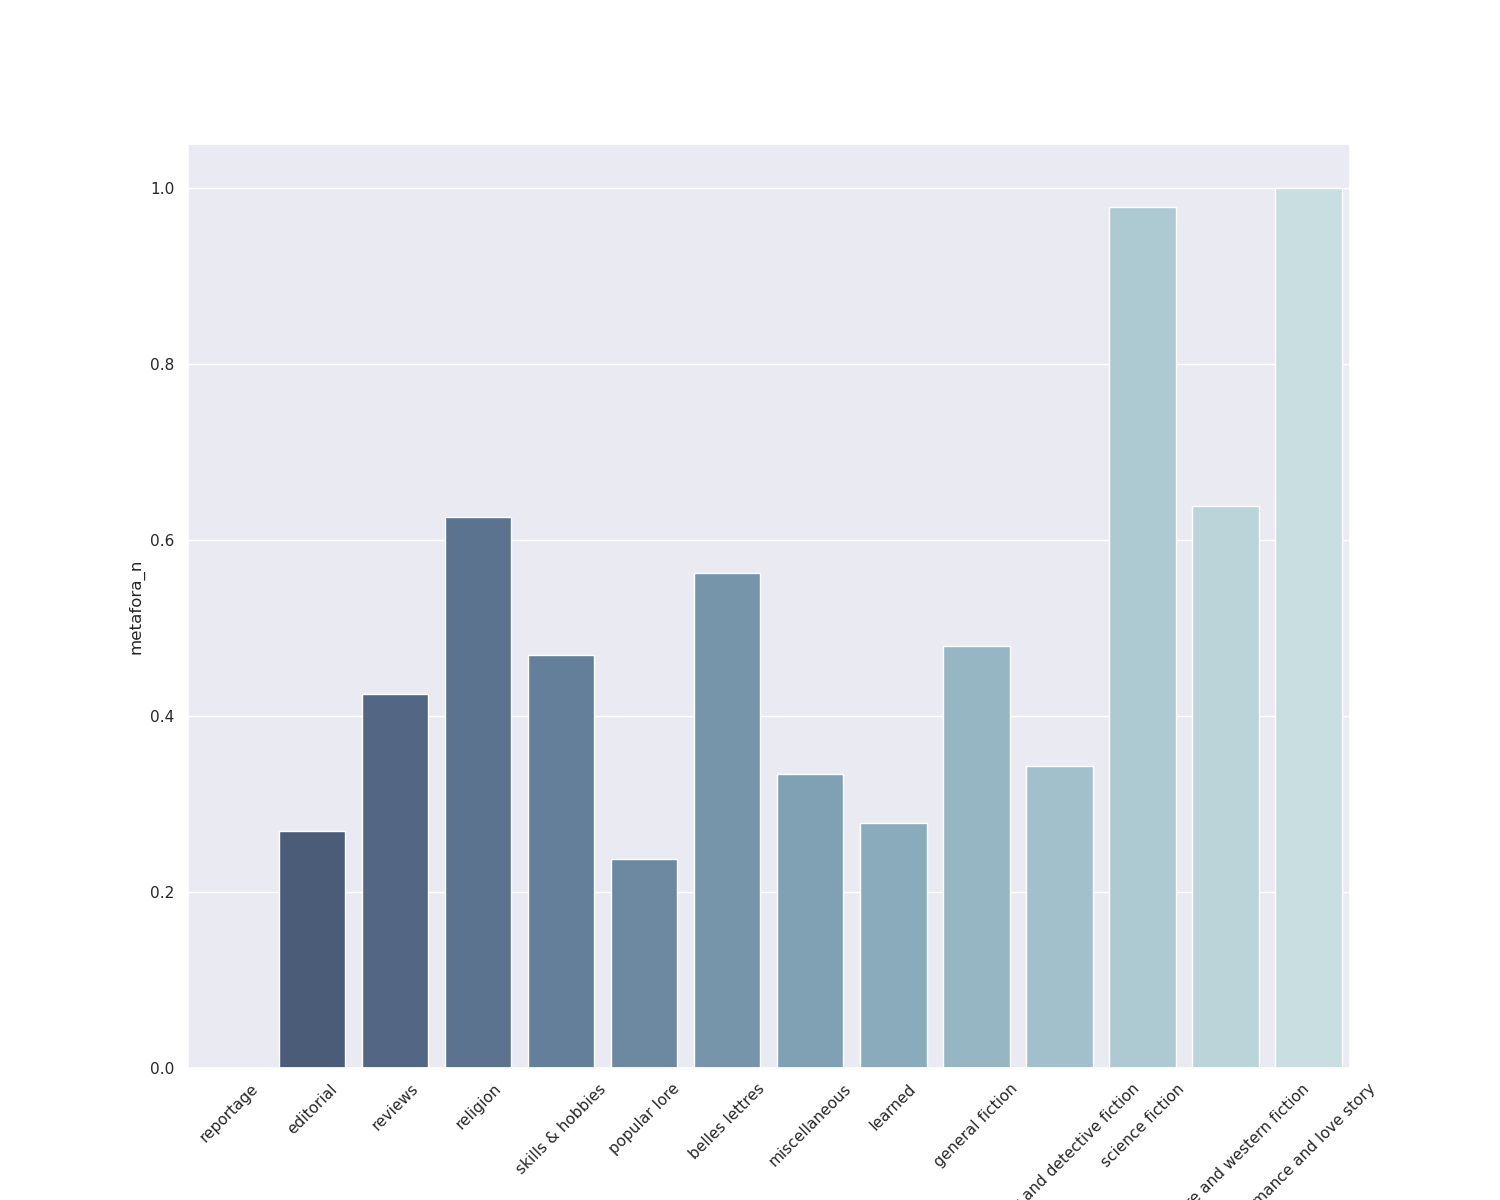
\includegraphics[width=.45\linewidth]{./resultados/graphs/muestra/c4_metafora.png}
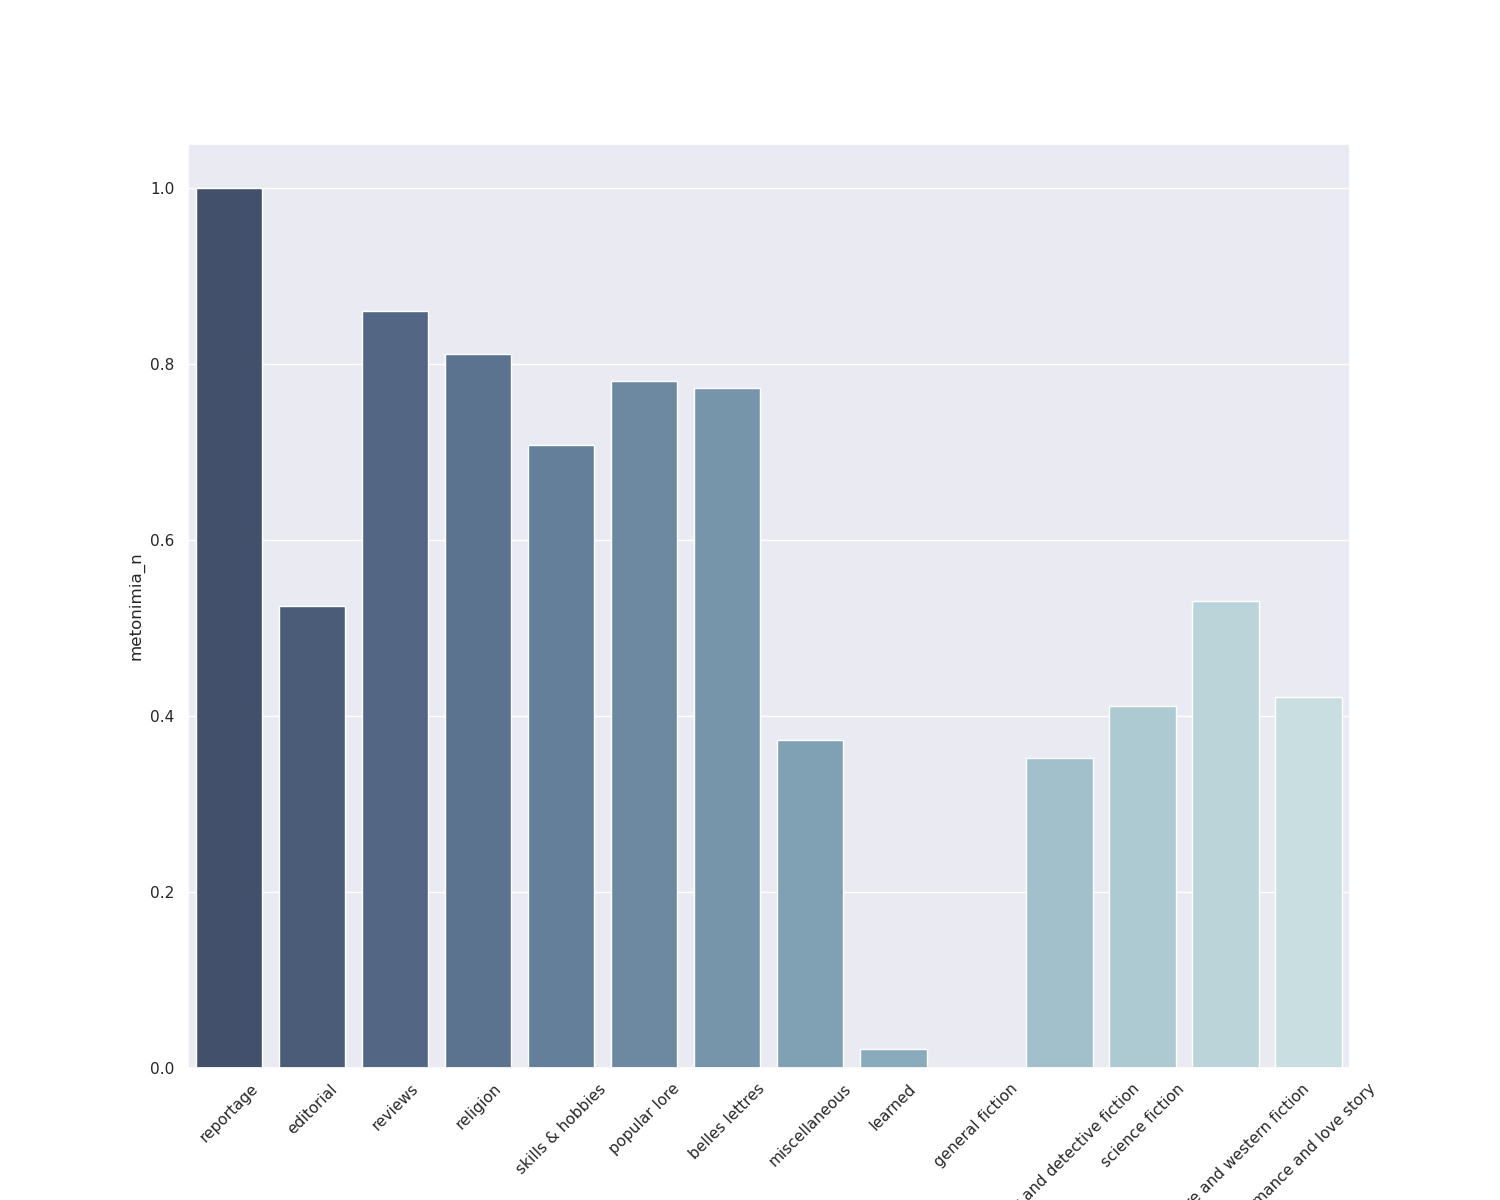
\includegraphics[width=.45\linewidth]{./resultados/graphs/muestra/c4_metonimia.png}
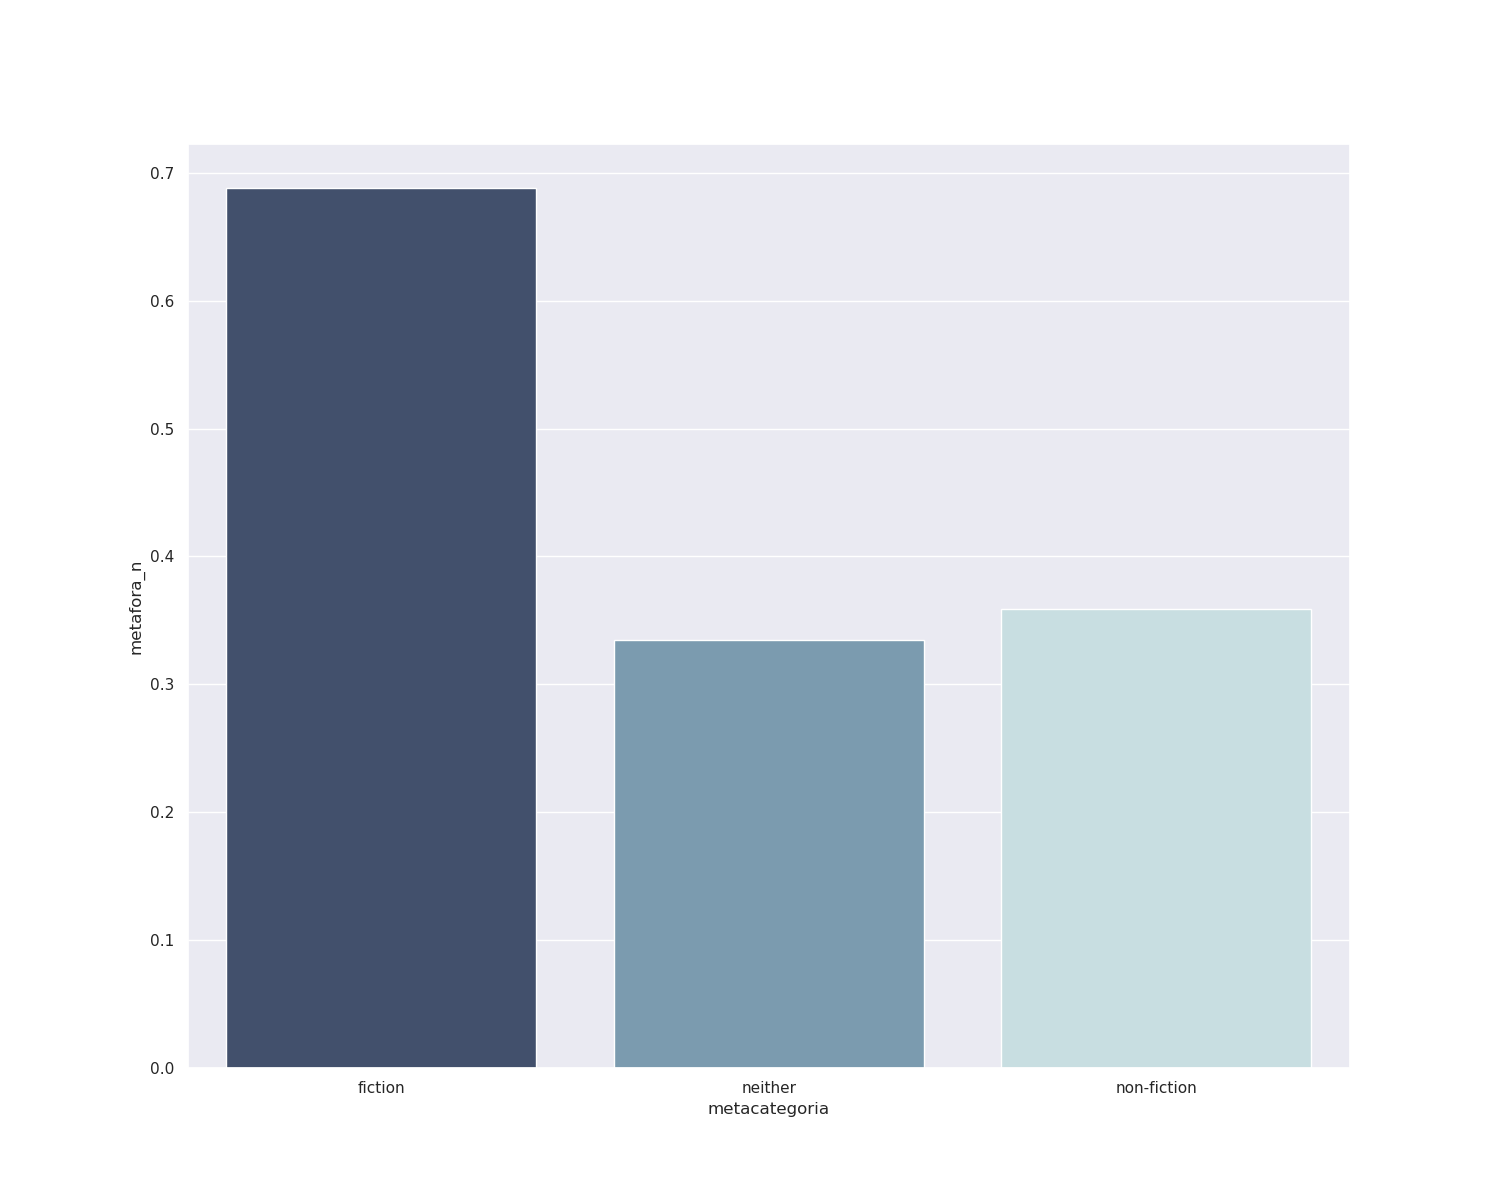
\includegraphics[width=.45\linewidth]{./resultados/graphs/meta/c4_metacategoria_metafora.png}
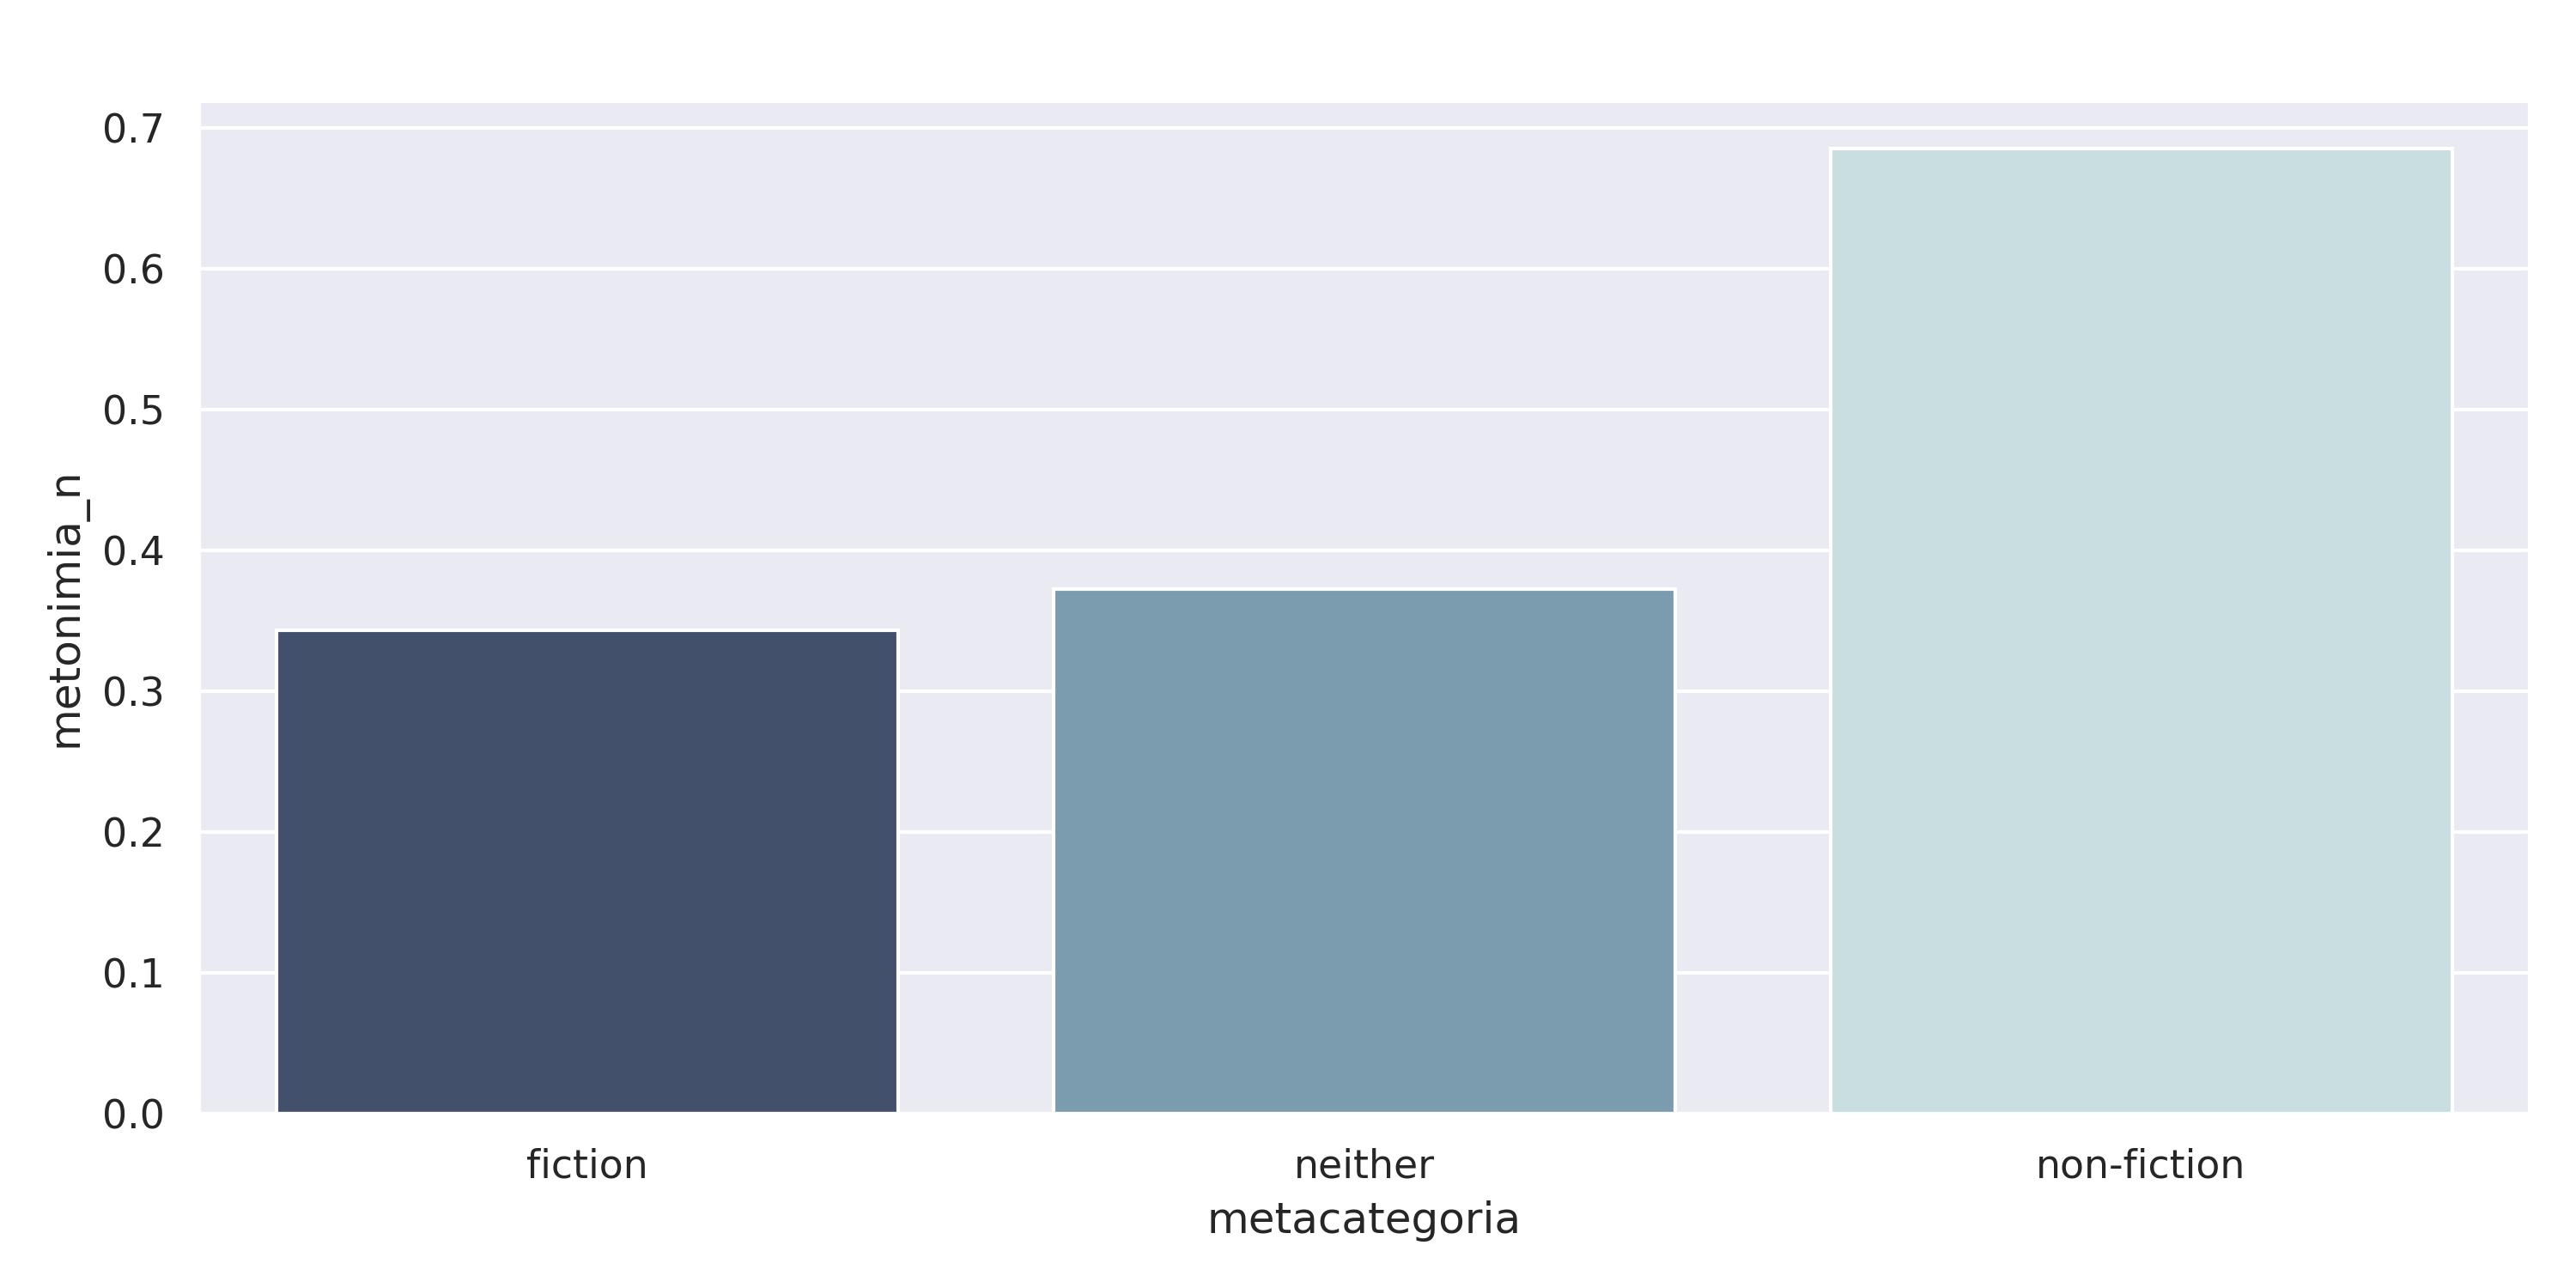
\includegraphics[width=.45\linewidth]{./resultados/graphs/meta/c4_metacategoria_metonimia.png}
\caption{\label{fig:c4_resultados}Resultados muestra 4}
\end{figure}

\begin{figure}[H]
\centering
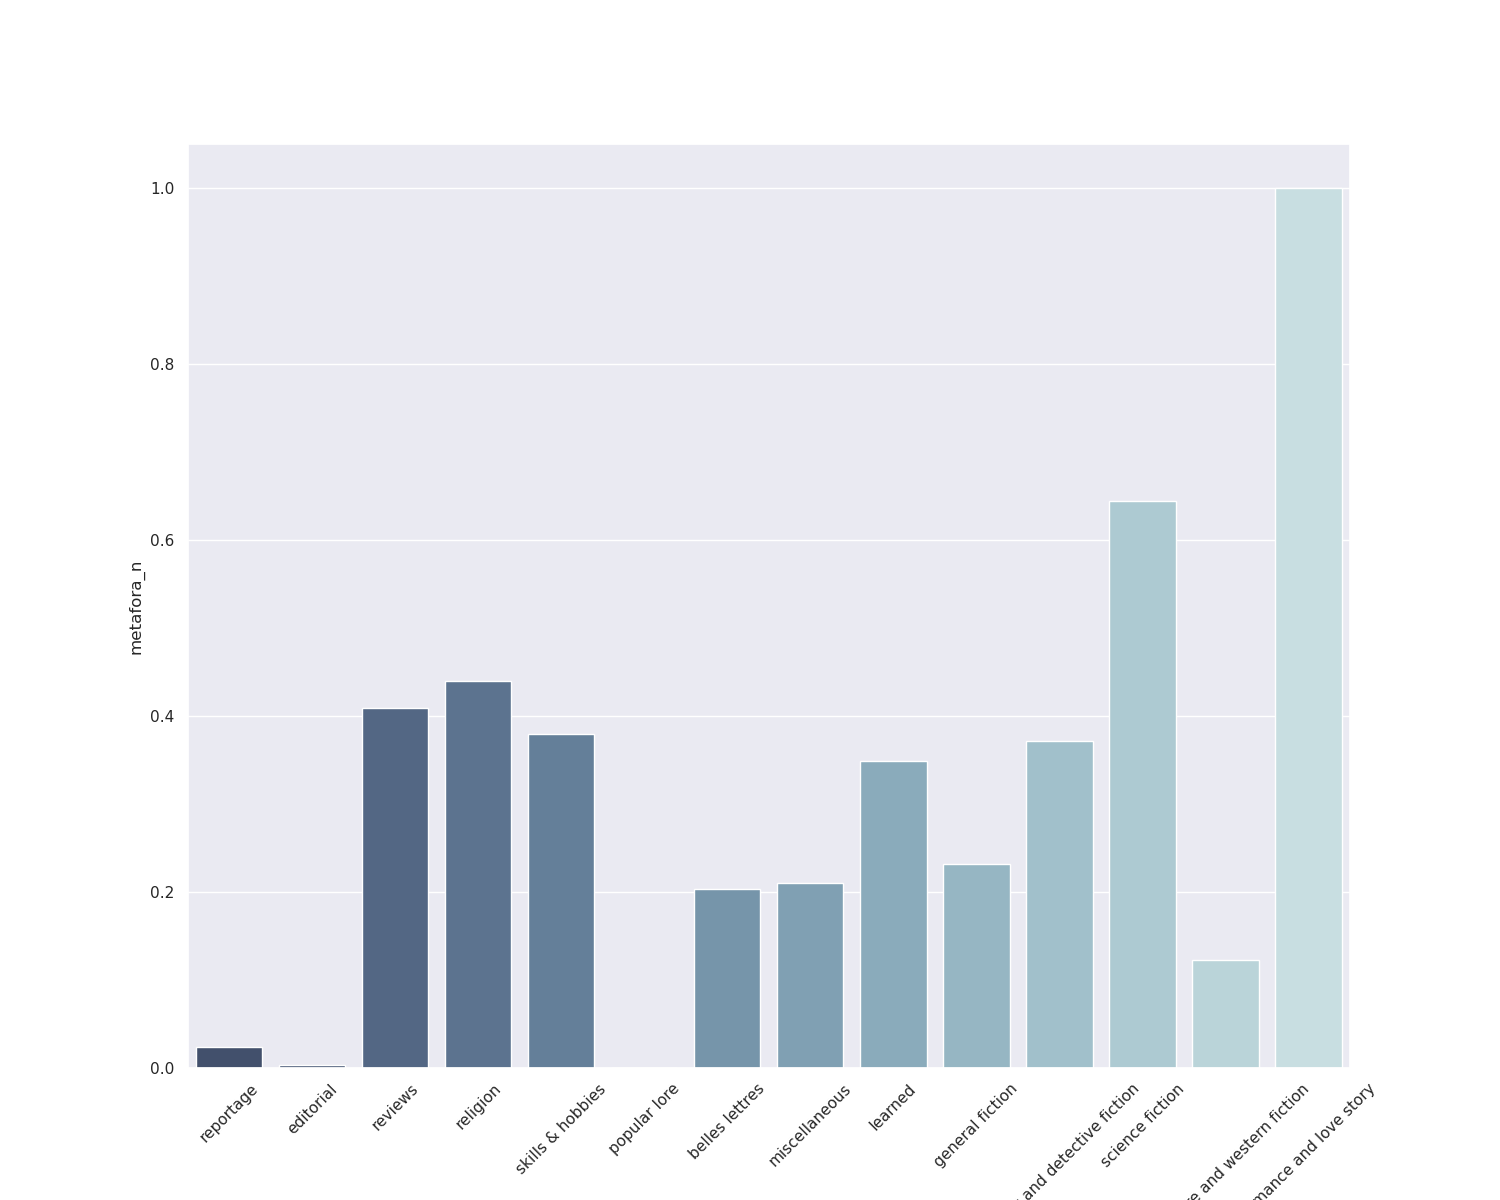
\includegraphics[width=.45\linewidth]{./resultados/graphs/muestra/c5_metafora.png}
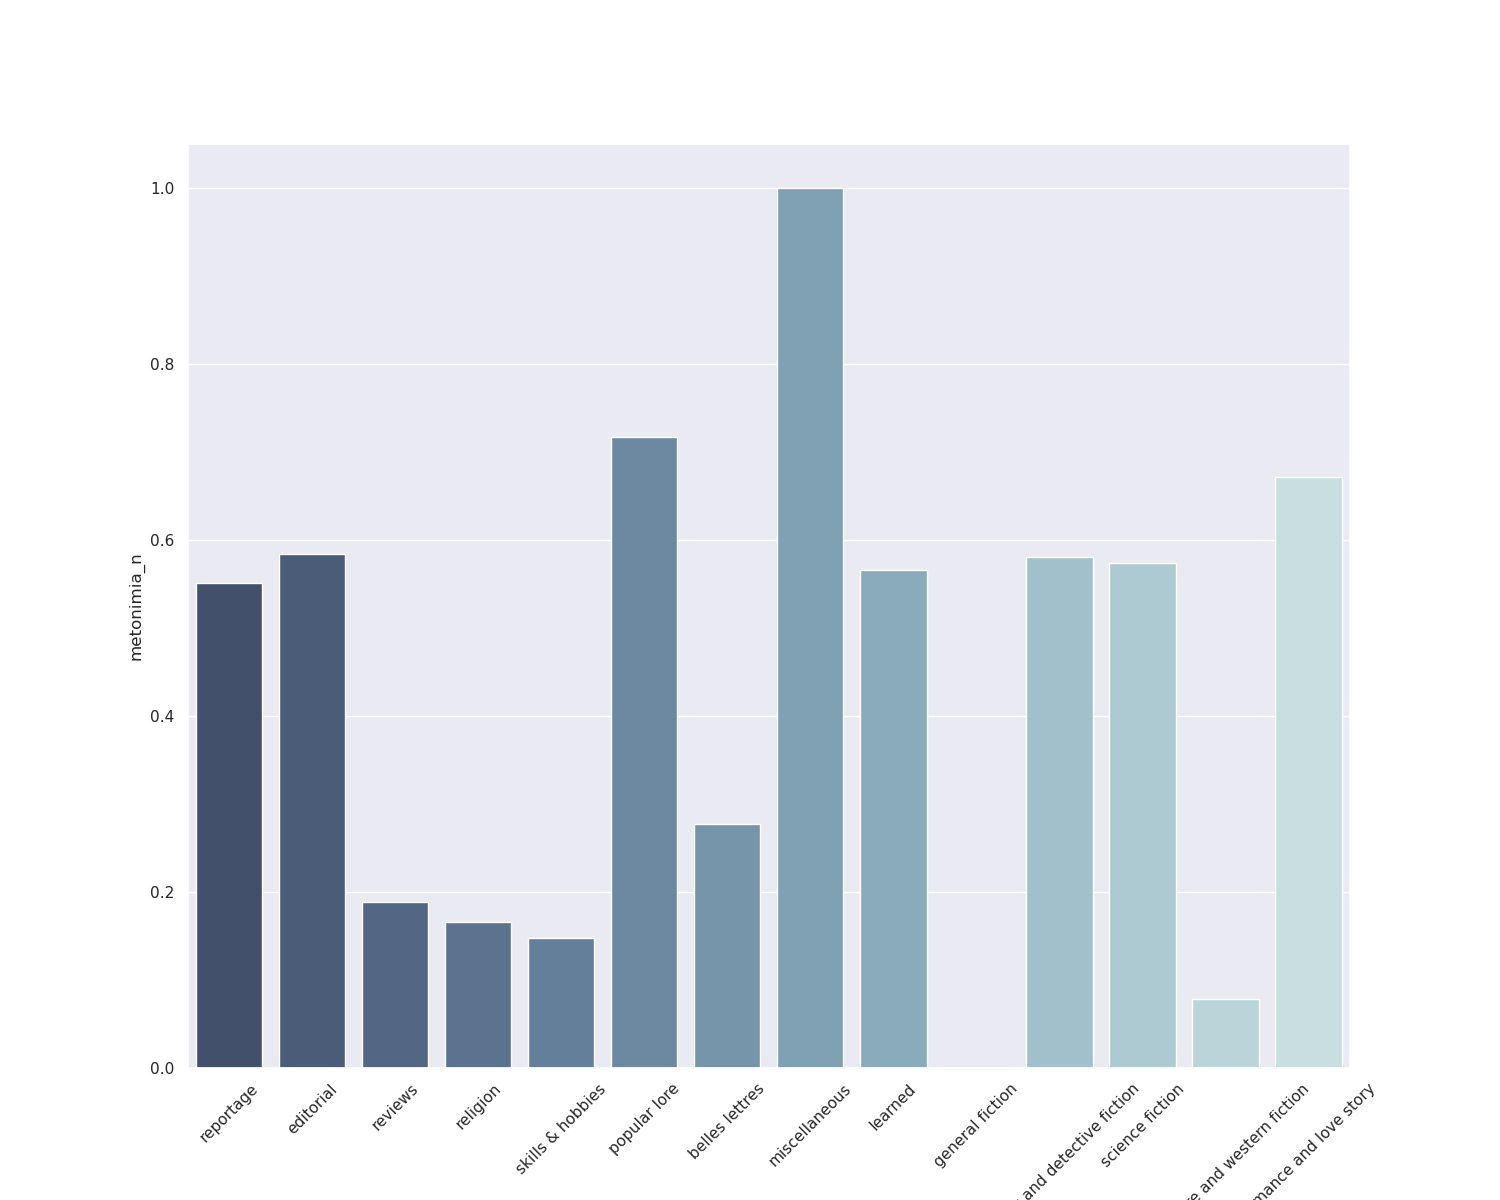
\includegraphics[width=.45\linewidth]{./resultados/graphs/muestra/c5_metonimia.png}
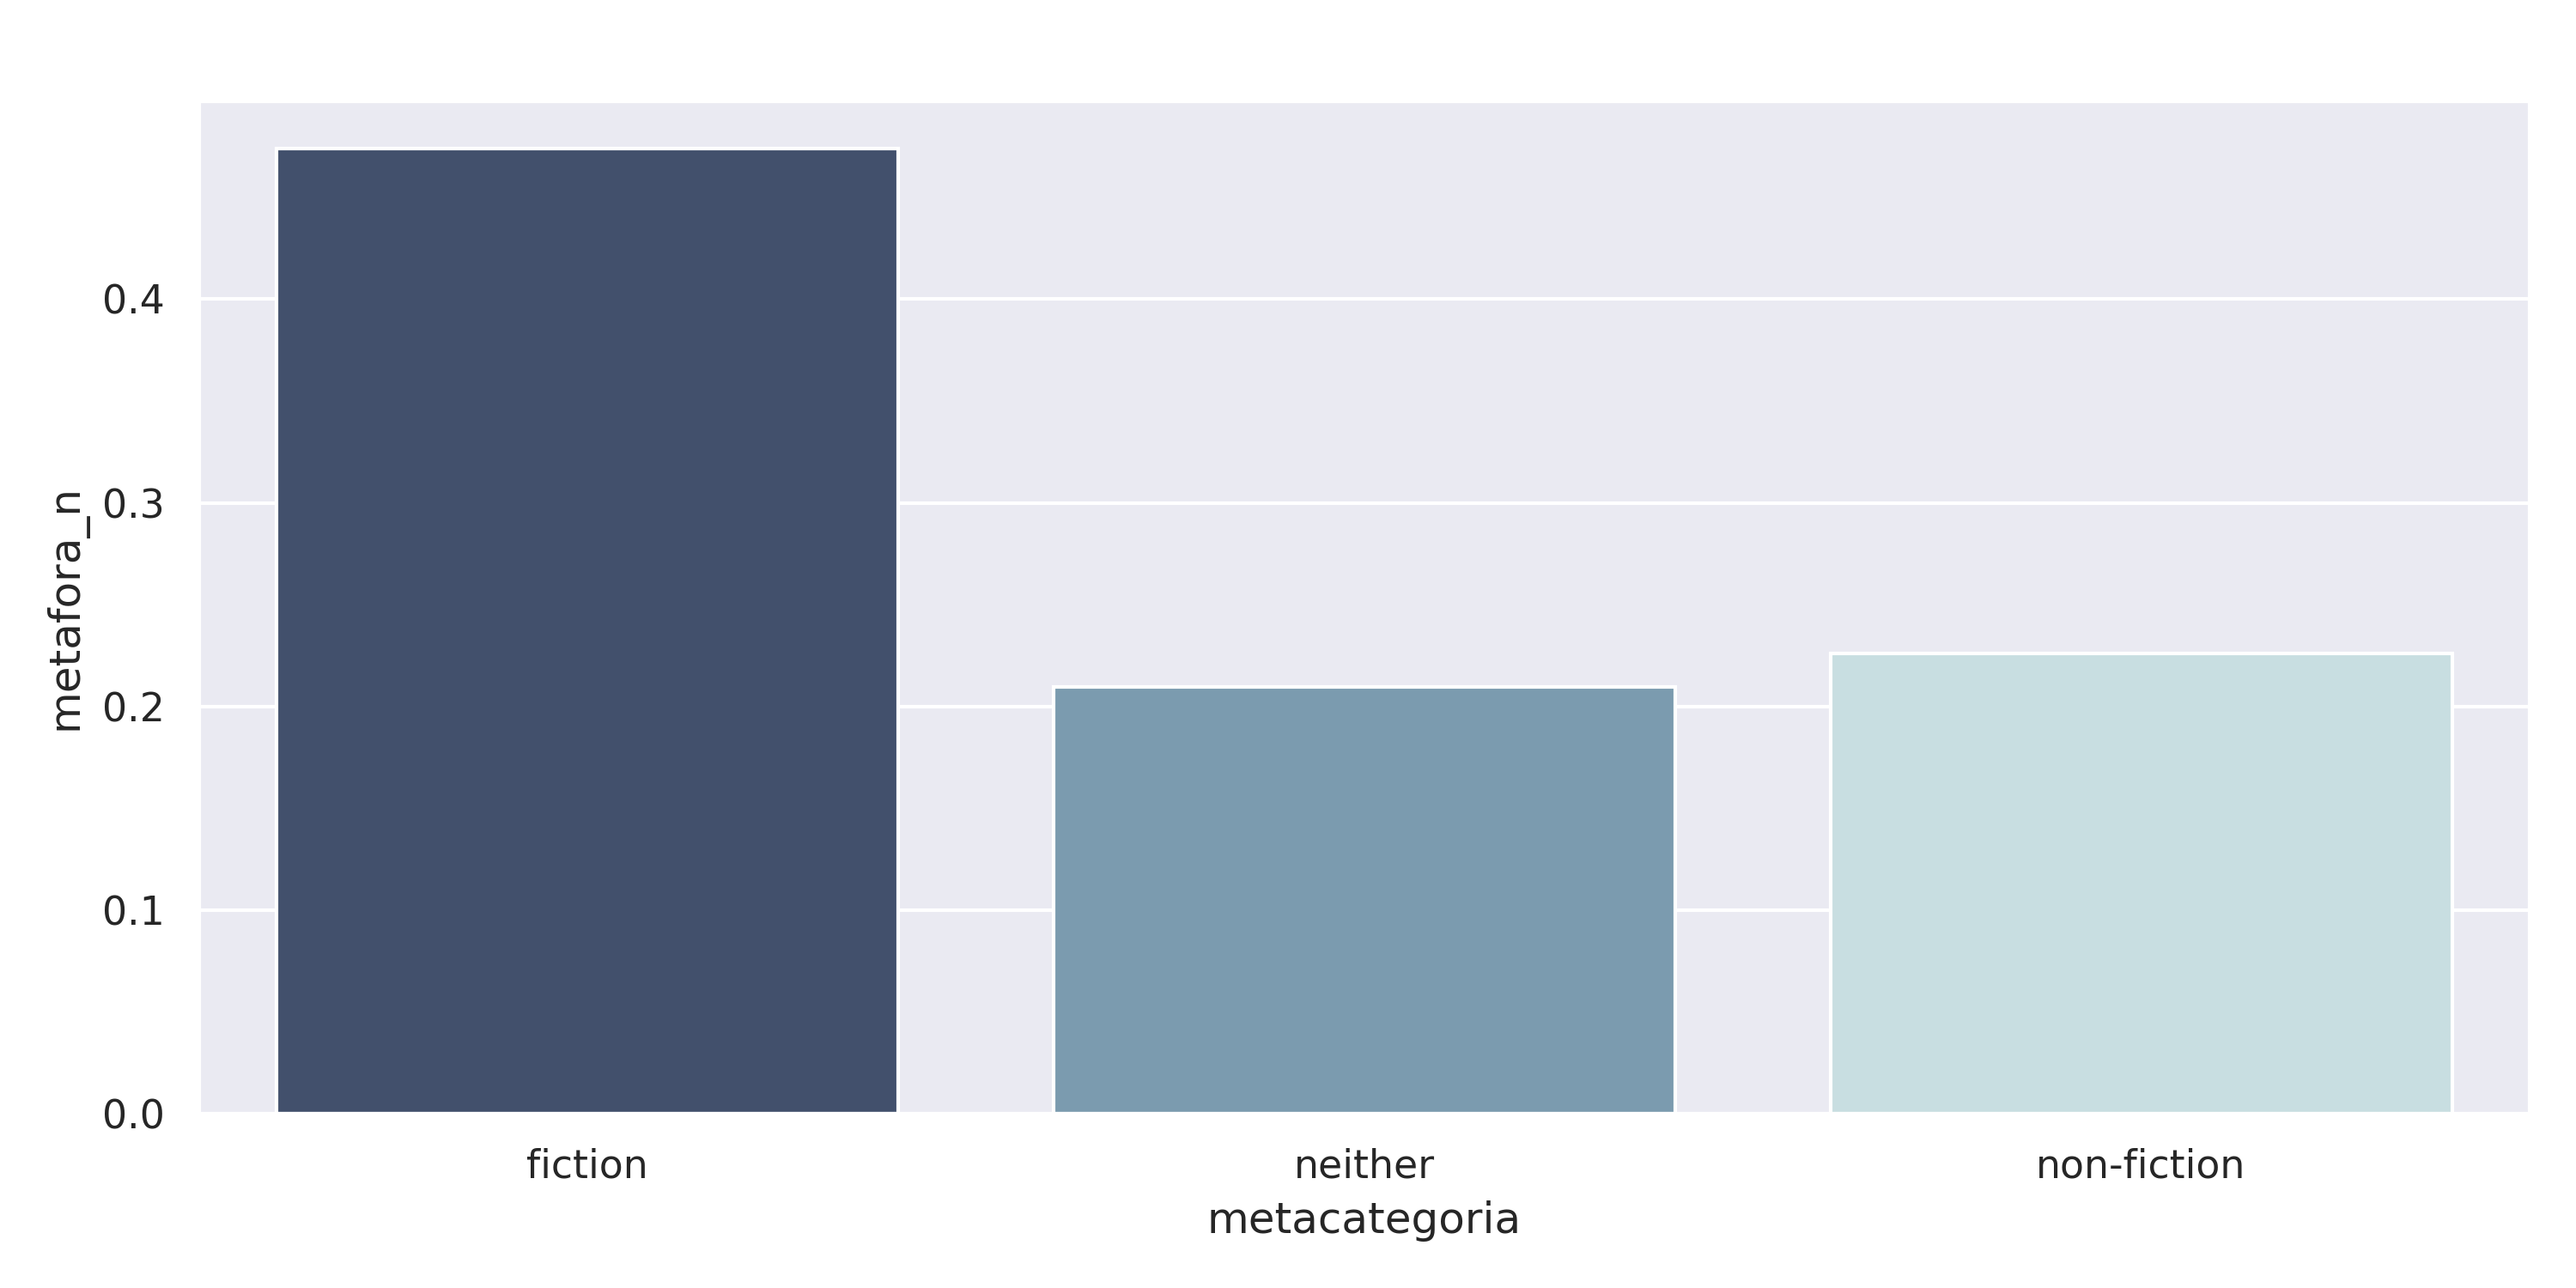
\includegraphics[width=.45\linewidth]{./resultados/graphs/meta/c5_metacategoria_metafora.png}
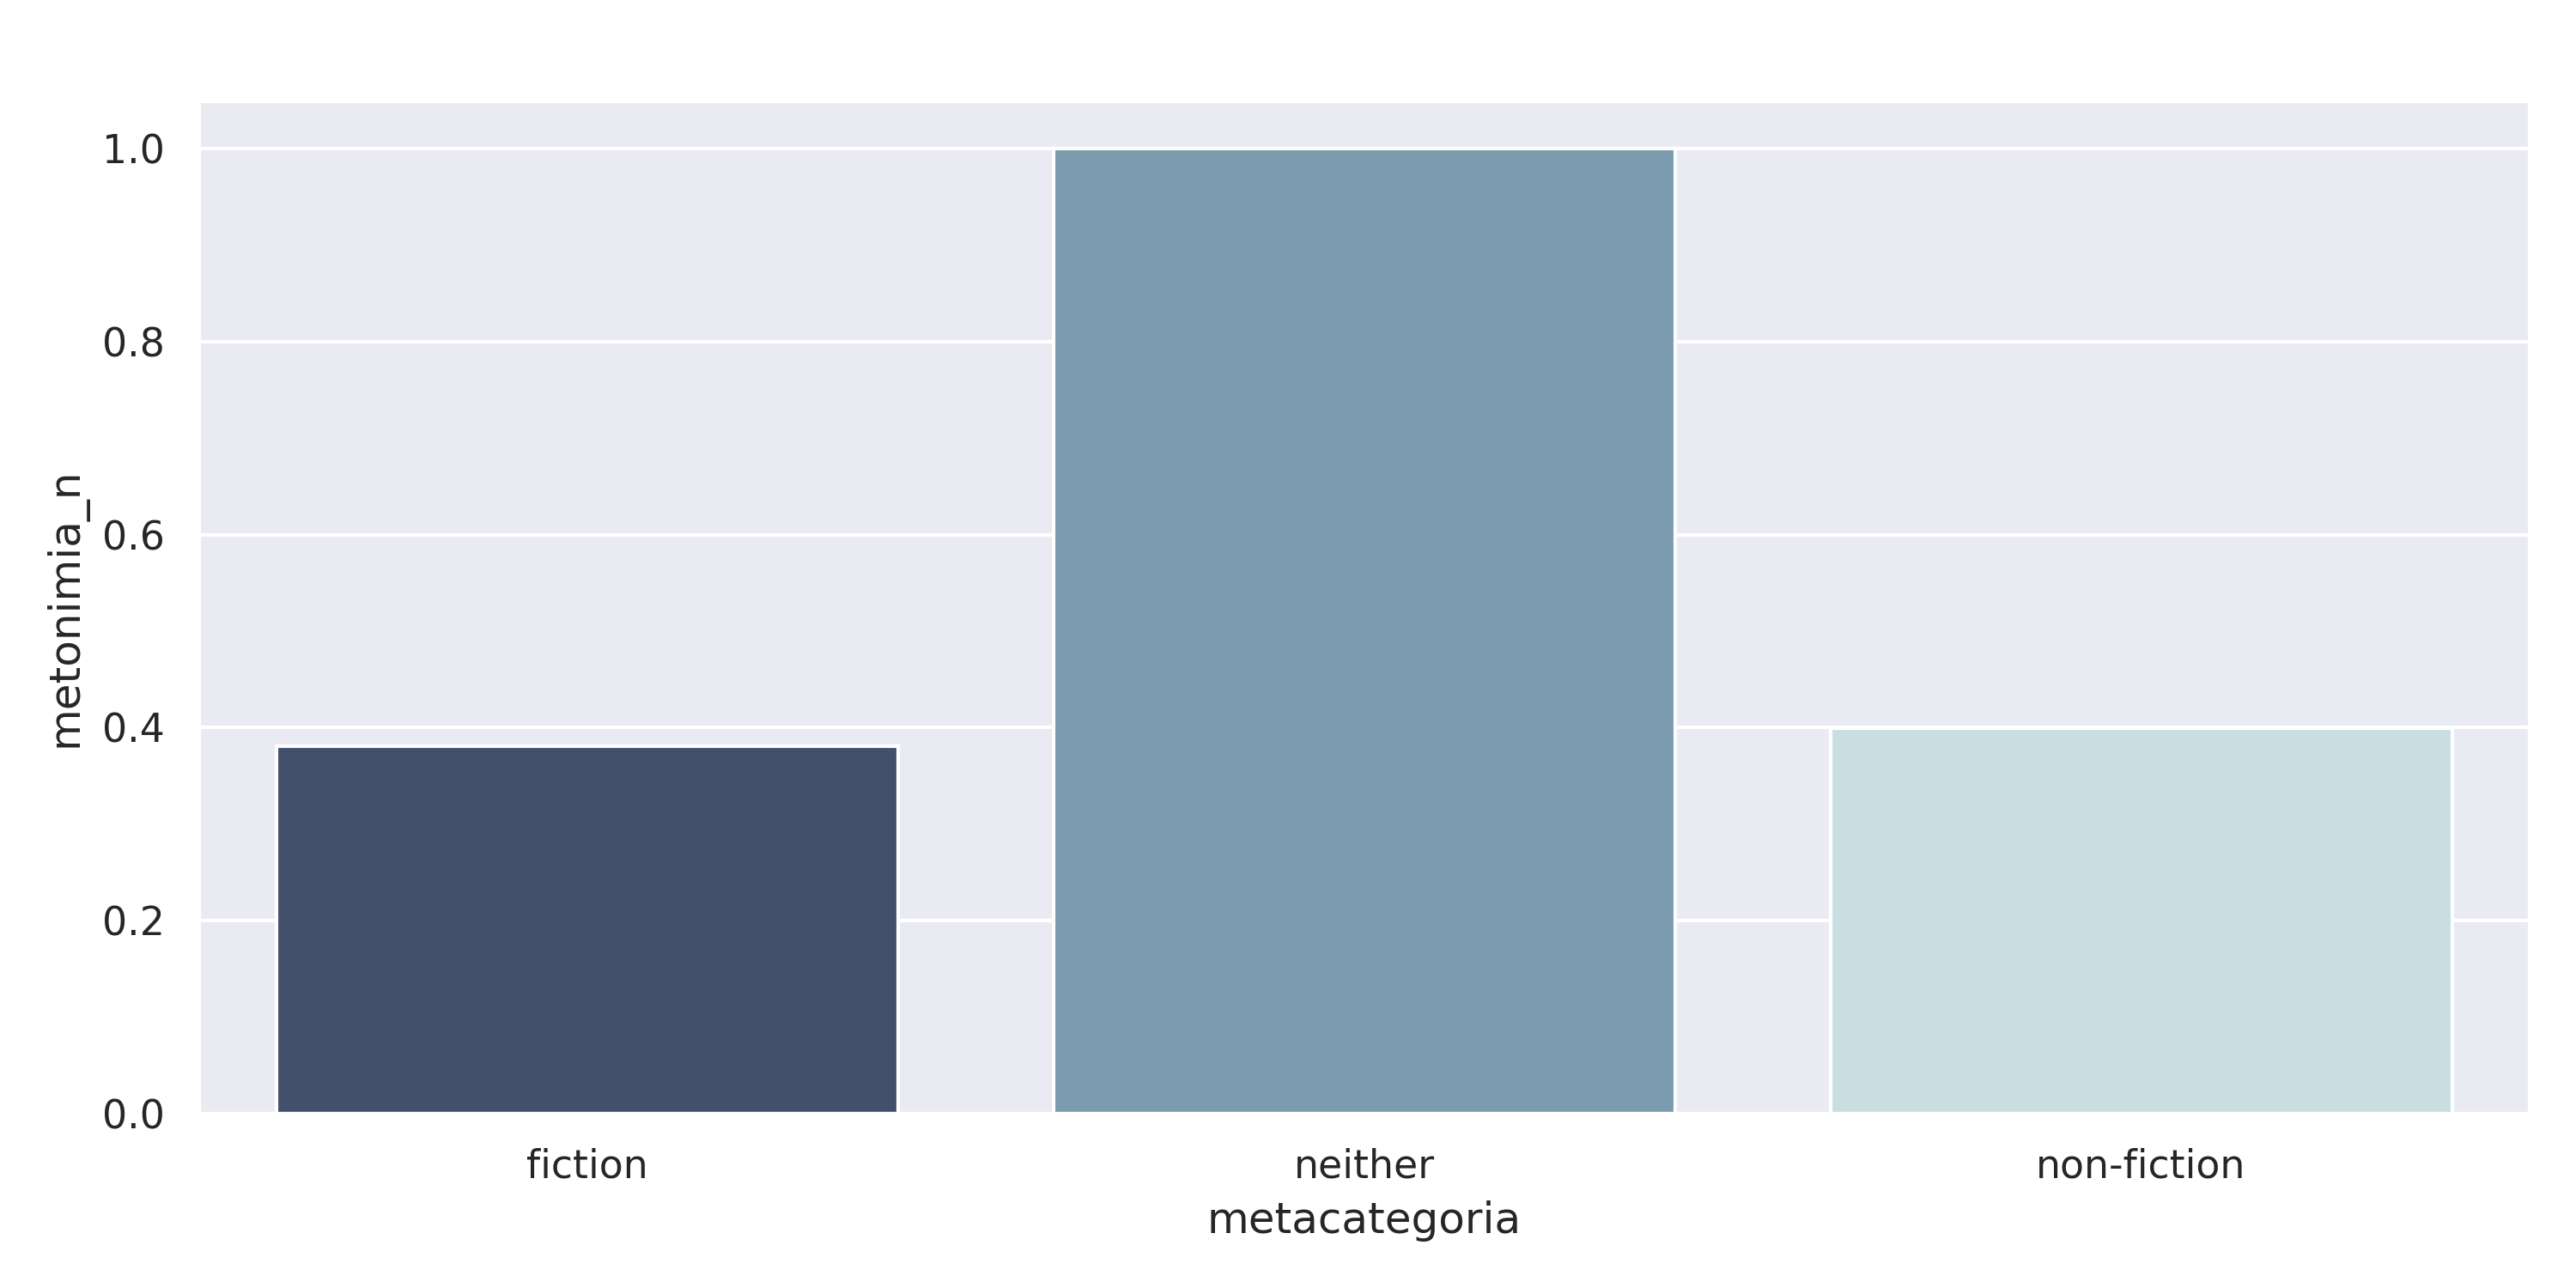
\includegraphics[width=.45\linewidth]{./resultados/graphs/meta/c5_metacategoria_metonimia.png}
\caption{\label{fig:c5_resultados}Resultados muestra 5}
\end{figure}


\subsubsection{Gráficos totales}
\label{sec:org0e8024f}
En esta sección se presentan los gráficos para el \textbf{índice metafórico} y el \textbf{índice metonímico}
teniendo en cuenta su comportamiento a lo largo de todos los corpus objetivos. Por lo tanto,
cada boxplot está constuido de 5 muestras (correspondientes a 1 representante de cada corpus
objetivo) para cada categoría, por lo que se puede obtener una noción más clara del IQR, la mediana
, los datos atípicos en cada categoría y metacategoría.

La visualización del comportamiento de los indicadores será necesaria para las Conclusiones (\ref{sec:org7f5f48c}).

\begin{figure}[H]
\centering
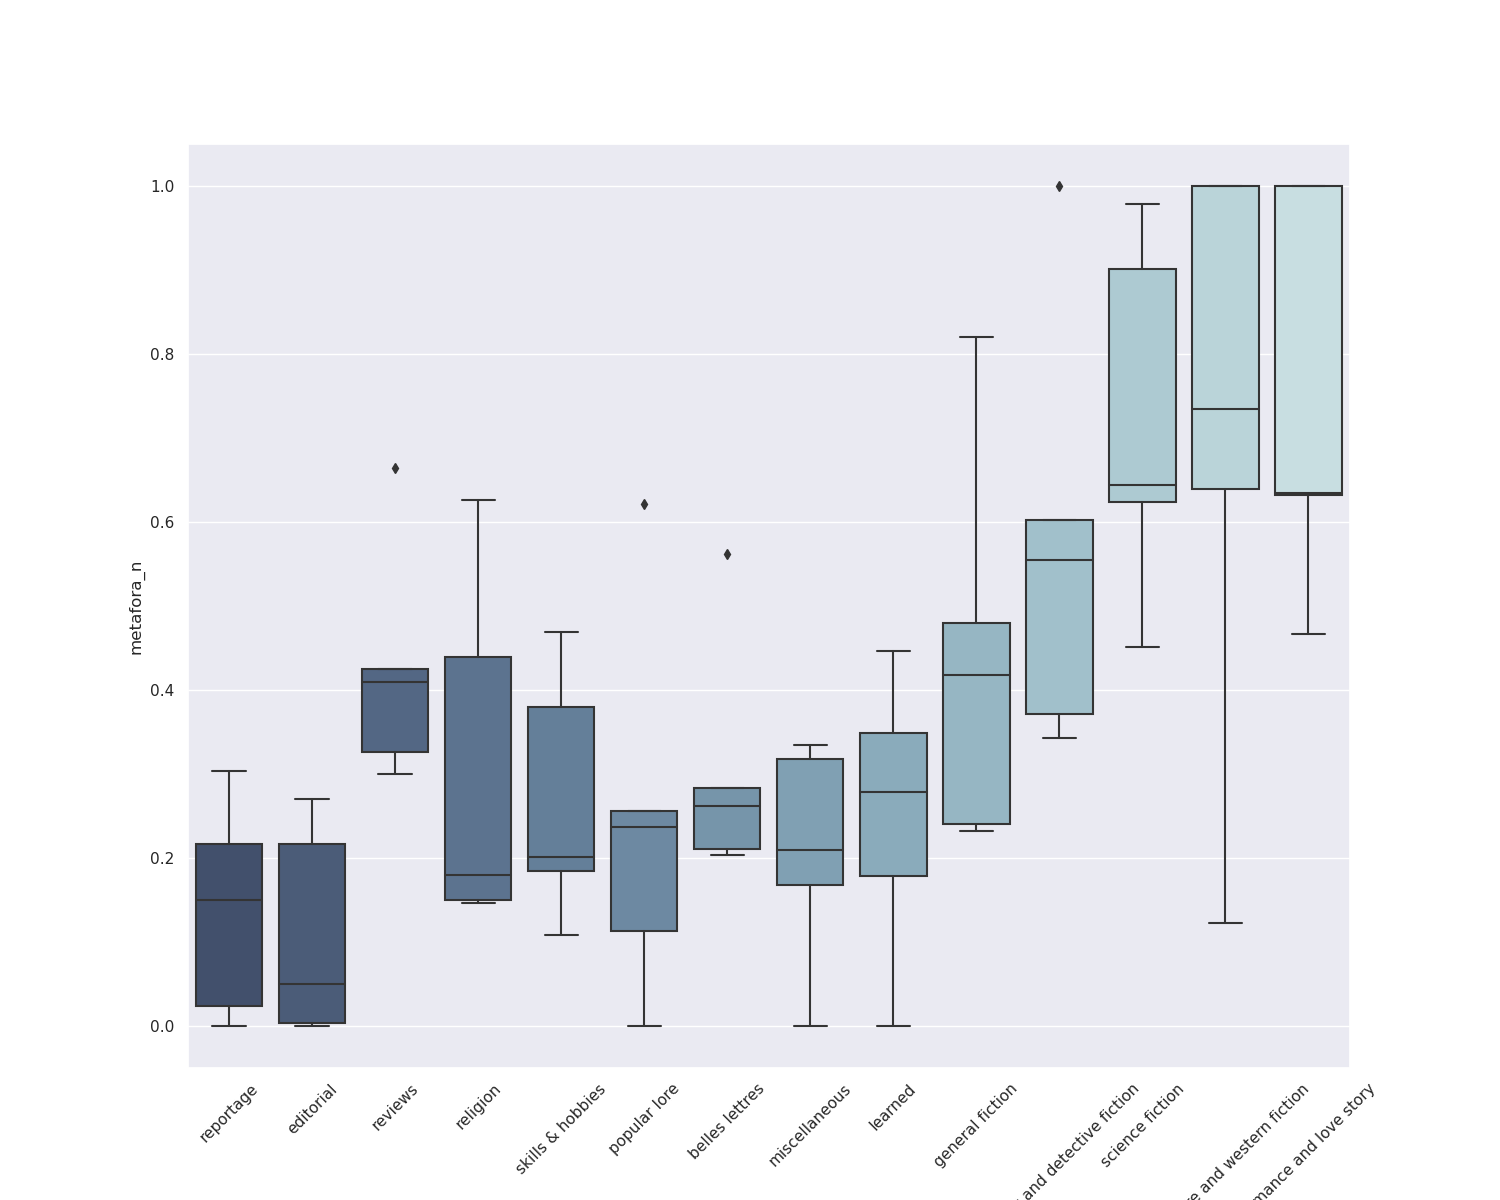
\includegraphics[width=0.9\linewidth]{./resultados/graphs/total/accum_cat_metafora.png}
\caption{\label{fig:metafora_categorias} Índice metafórico por categorías a través de las muestras }
\end{figure}
\begin{figure}[H]
\centering
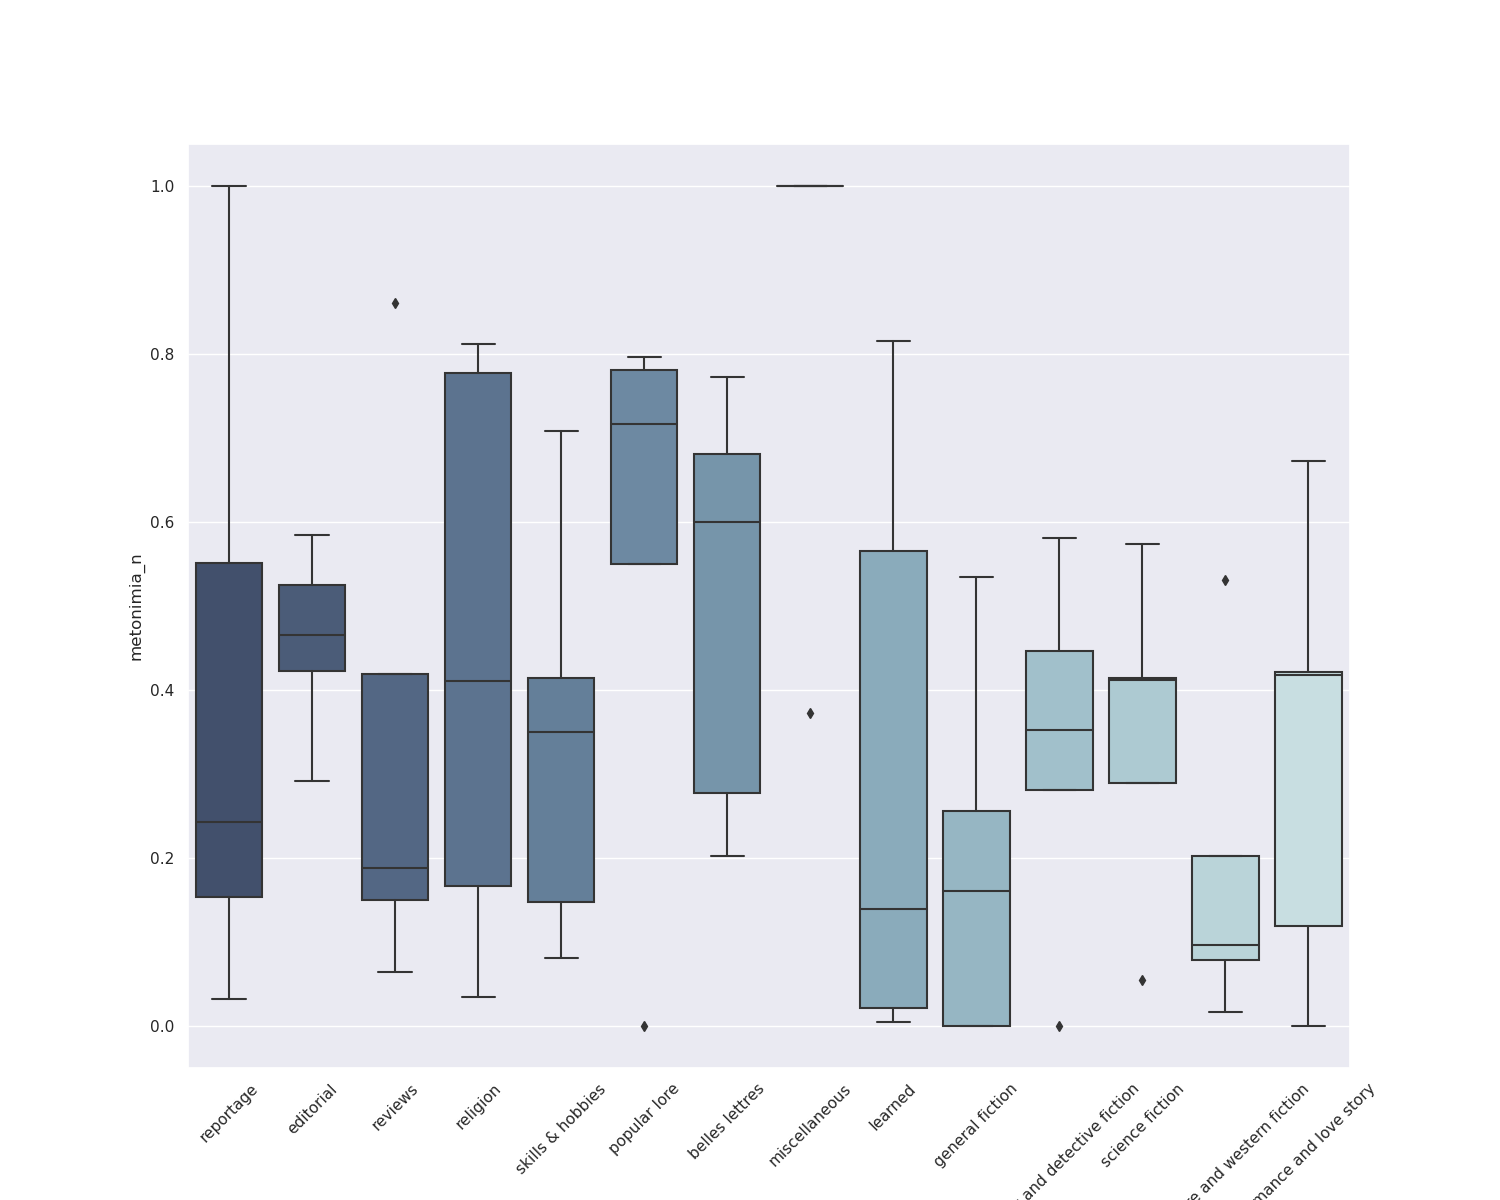
\includegraphics[width=0.9\linewidth]{./resultados/graphs/total/accum_cat_metonimia.png}
\caption{\label{fig:metonimia_categorias} Índice metonímico por categorías a través de las muestras  }
\end{figure}
\begin{figure}[H]
\centering
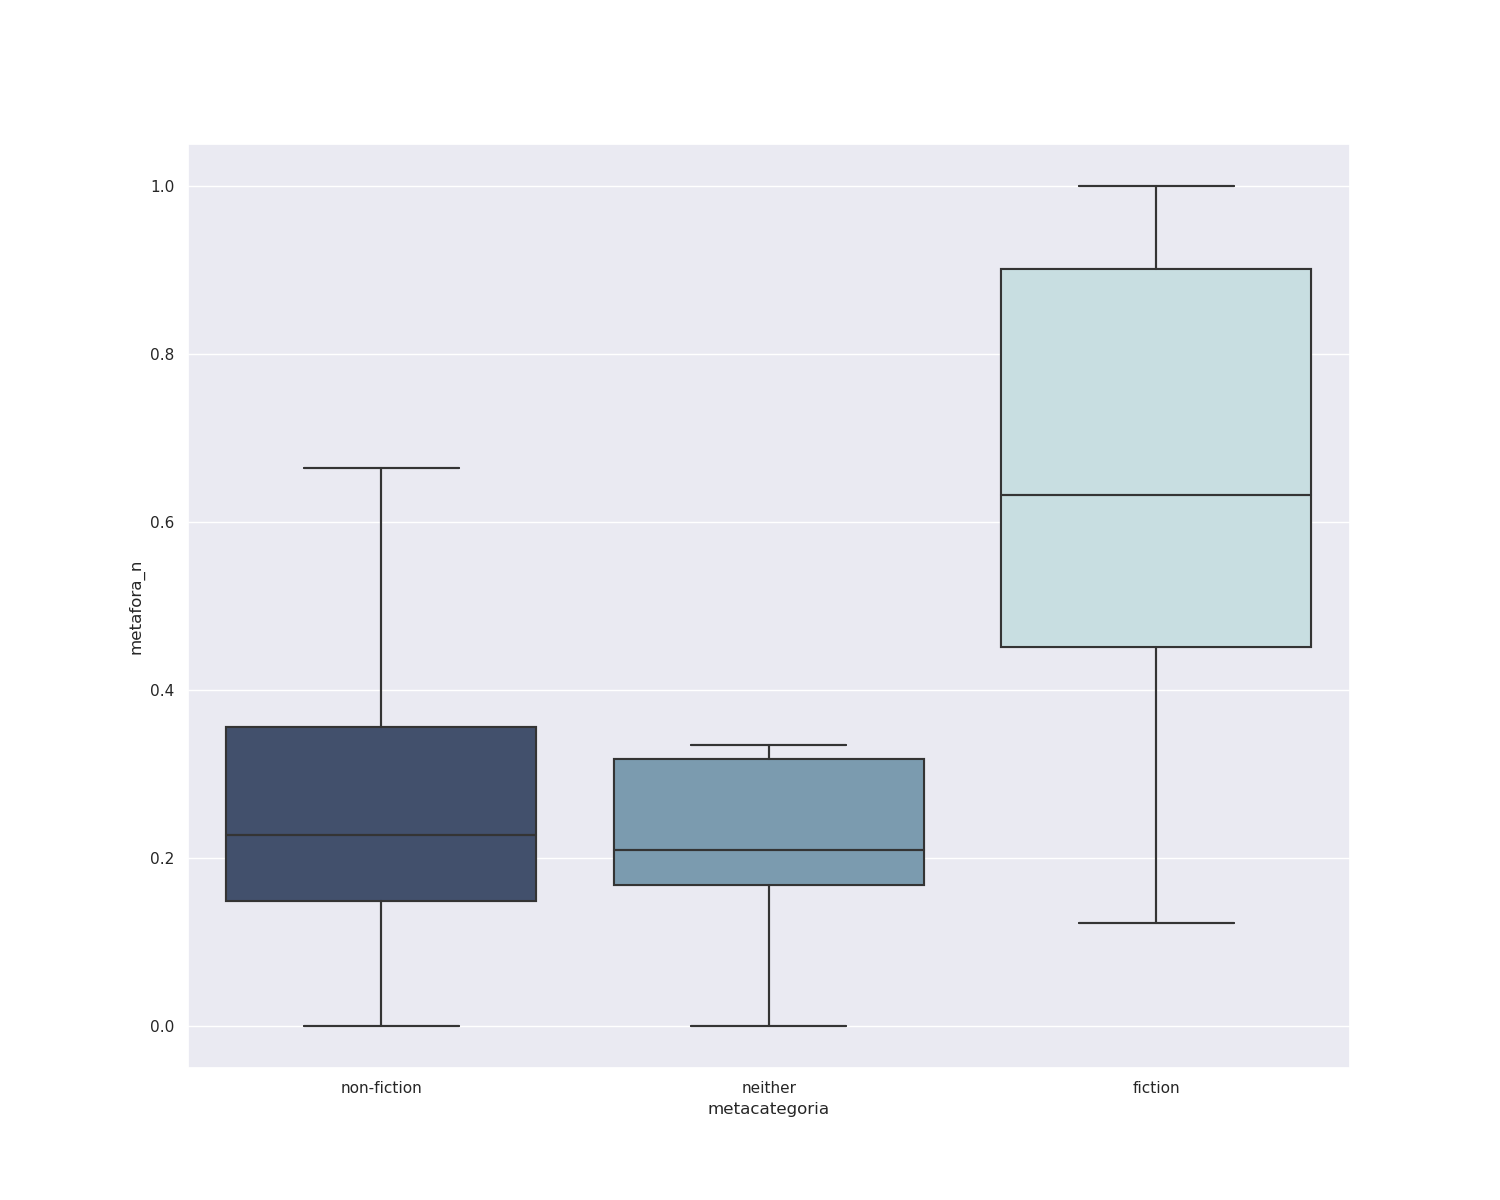
\includegraphics[width=0.9\linewidth]{./resultados/graphs/total/metafora_total.png}
\caption{\label{fig:metafora_total} Índice metafórico por metacategorías a través de muestras }
\end{figure}

\begin{figure}[H]
\centering
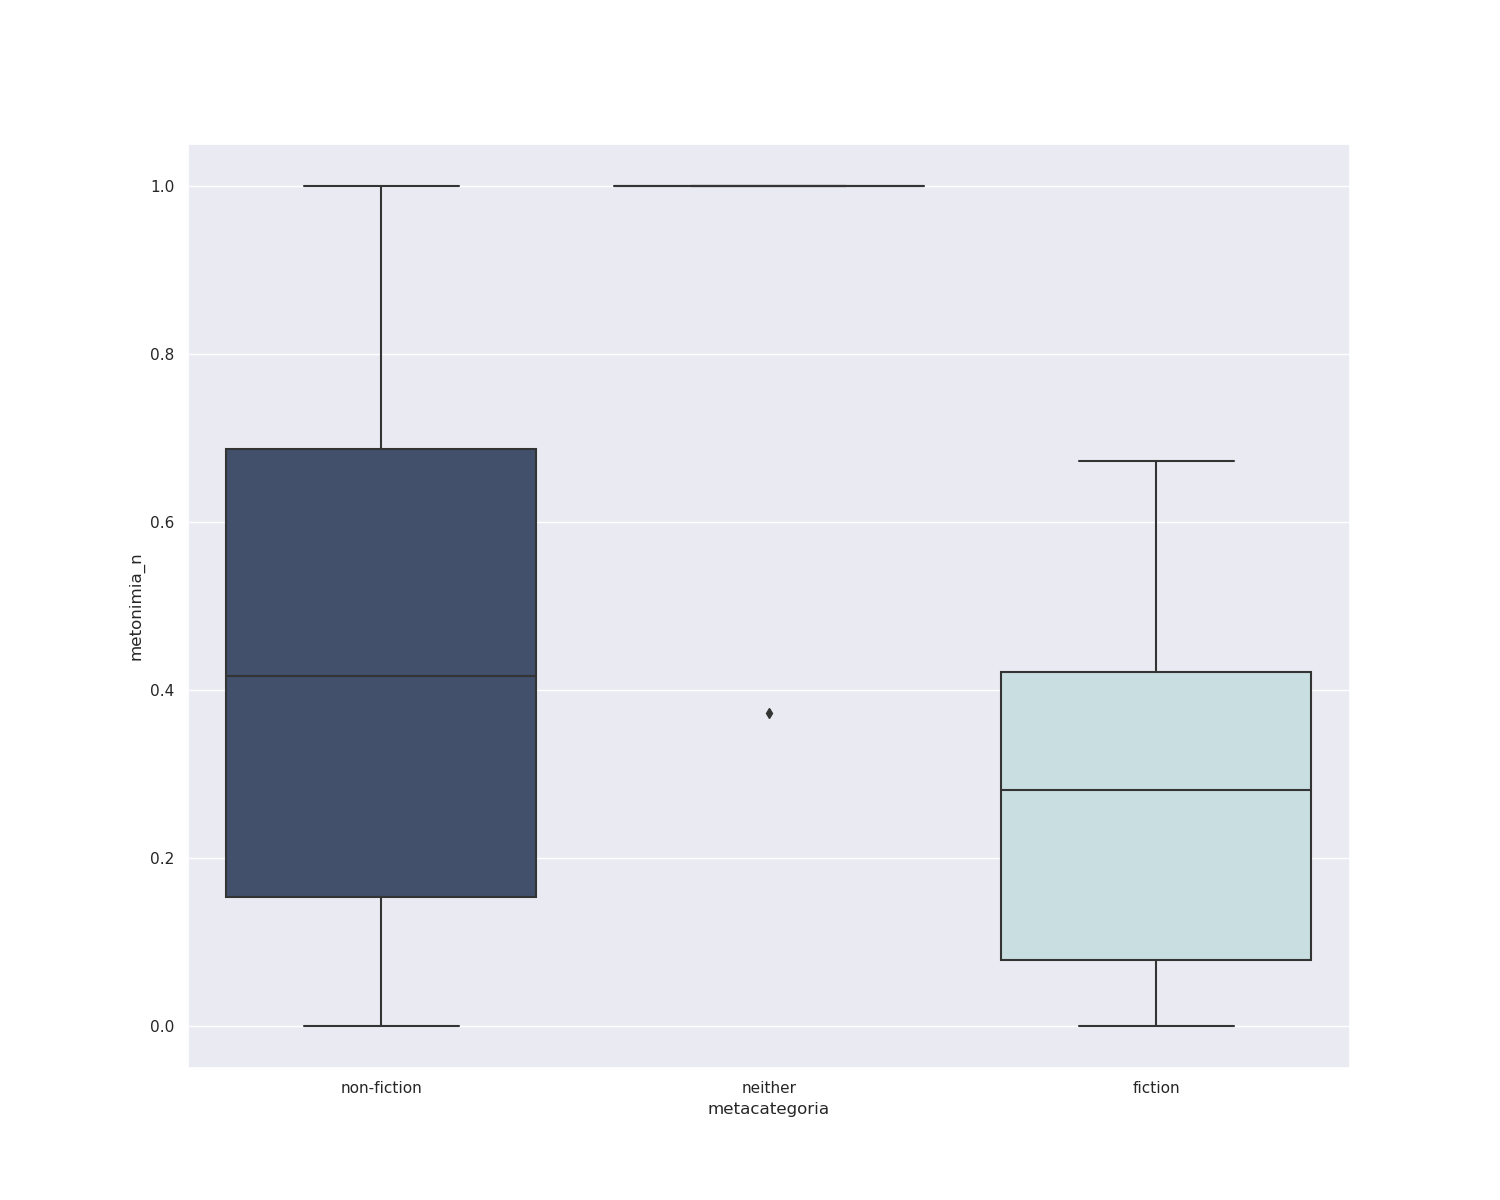
\includegraphics[width=0.9\linewidth]{./resultados/graphs/total/metonimia_total.png}
\caption{\label{fig:metonimia_total} Índice metonimica por metacategoria a través de muestras }
\end{figure}

\subsection{Evaluación}
\label{sec:orgf2133af}
Según lo contempla el proceso de analítica de datos (ver sección \ref{sec:org8962c76}),
es necesario someter a prueba los modelos postulados. Sin embargo, como el modelo propuesto
no se enmarca dentro de Machine Learning, no se dispone de un algoritmo de clasificación
per se, que luego de pueda evaluar con un set de validación.

Sin embargo, teniendo en cuenta los hipótesis planteadas en la sección \ref{sec:org5b898bb},
se pueden realizar pruebas estadísticas que pueden aportar una fundamentación cuantitativa,
para las hipótesis que lo permitan.

Así, para la H\textsubscript{1}, que plantea que las metacategorías de ficción y no ficción tengan un
índice metaforico significativamente distinto se formula una prueba ANOVA, a lo largo de
todas las muestras, entre los textos de ficción y no ficción, con el siguiente resultado:

\begin{verbatim}
>>> anova_metafora
F_onewayResult(statistic=51.510567153609514, pvalue=9.812579375438188e-10)

\end{verbatim}

Por lo tanto, se como el valor-p para la prueba ANOVA es inferior a 0.01 y
el estadístico \(F\) es muy alto, se puede afirmar que el algoritmo genera valores
significativamente distintos entre las metacategorías de ficción y no ficción,
con una confianza mayor al 99\%.

Así mismo, si se hace una prueba ANOVA para el índice metonímico para las
metacategorías de ficción y no ficción se obtiene que:


\begin{verbatim}
  >>> anova_metonimia
F_onewayResult(statistic=4.327636012671773, pvalue=0.04157136345702674)

\end{verbatim}

Por lo tanto, como el valor-p para la prueba es inferior a 0.05 y el estadístico
\(F\) es más alto que 1, se puede aformar que el algoritmo genera valores
significativamente distintos entre las metacategorias de ficción y no ficción
con una confianza de 95\%.


\section{CONCLUSIONES}
\label{sec:org7f5f48c}

Para concluir el presente trabajo, primero se señalarán los resultados
del experimento frente a las hipótesis planteadas y los hallazgos.
Posteriormente, se expondrán las críticas posibles al modelo
planteado. Por último, se señalaran trabajos futuros para profundizar
más en la pregunta de investigación.

\subsection{Las hipótesis planteadas}
\label{sec:org36757f6}

Para la hipótesis H\textsubscript{1} se observa en la figura
\ref{fig:metafora_total} que el índice metafórico es, en promedio, más
alto para las categorias de no ficción que para las categorias de no
ficción, a lo largo las 5 muestras. De hecho, en promedio, las obras
de ficción reportan un índice metafórico 252\% más alto (0.635572) que
las de no ficción (0.256140). Esto es consistente con la intuición,
que nos dicta que en las obras de ficción se hace uso de un
vocabulario más amplio y distinguido, lo que aporta más al índice
metafórico.

En cuanto a la hipótesis H\textsubscript{2}, las medias para las categorias
\emph{reportage} y \emph{editorial} son cercanas (0.14 y 0.11,
respectivamente). En el gráfico \ref{fig:metafora_categorias} se puede
apreciar que el rango interquartil (IRQ) es muy similar. Esto es
consistente con el resultado esperado, puesto que estas dos categorías
son similares entre sí: ambas están conformadas por textos que
aparecieron en publicaciones periódicas. Como comparten muchos
parámetros linguísticos similares en cuanto al vocabulario (misma
audiencia, año, medio, etc), su indice metafórico debe ser similar a
lo largo de las muestras.

Luego, para la hipótesis H\textsubscript{3}, se puede observar que la categoría
\emph{Belles Lettres} es la tercera con índice metafórico más alto
(con un 0.30). Queda por debajo de \emph{Religion} (0.31) por un punto porcentual y de
\emph{Reviews} (0.42). Este resultado no es el esperado, pero es
comprensible si se tiene en cuenta que la categoría \emph{Reviews} está
compuesta de críticas a obras de arte como música clásica, libros y
obras de teatro, cuyo vocabulario puede terminar aportando más al
índice metafórico que las biografías y cartas de la categoría \emph{Belles
Lettres}.

Por último, para la hipótesis H\textsubscript{4}, se observa que la categoría
\emph{Learned} tiene el segundo índice de metonimia más bajo (0.31), luego
de (sorprendentemente) las categorias \emph{General Fiction} y \emph{Adventure \&
Western Fiction} (0.19 ambas). Si bien este resultado no es
estrictamente el esperado a lo largo de todas las categorias, la
hipótesis H\textsubscript{4} sí se cumple dentro de la metacategoría de
no-ficción. La hipótesis inicial se hizo sobre la base de que los
textos técnicos y científicos no deberían tener un enfasis en la
metonimia entre cada una de sus palabras.  Es decir, no debería haber
un énfasis en repetir sonidos a lo largo de una oración, puesto que
los factores de comunicación de Jakobson se centran en las funciones
conativa o fática.

\subsection{Hallazgos}
\label{sec:orgdc2d9d6}

Además de la validación de hipótesis iniciales, hubo un hallazgo
notable en el experimento que concierne al comportamiento del
índice metonímico. Se encontró que las obras de no ficción tienen
en promedio un índice metonímico más álto (0.41) que las obras de
ficción (0.21), casi un 100\% más. Además, la metacategoría
'neither', que corresponde a una categoría difícil de categorizar,
el de los comunicados gubernamentales (la categoria 'miscellaneus'
en el Corpus de Brown), obtuvo el índice metonímico absolutamente
más alto (0.87).

Esto, visto cuantitativamente, parece apuntar a una relación
inversamente proporcional entre el índice metafórico y el índice
metonímico. Por otro lado, cualitativamente, esta observación
podría tener una implicación notable.  El hallazgo corresponde a
que Jakobson alude al 'emparentamiento' de los principios de
métafora y metonimia a dos movimientos artísticos: el Romanticismo
(metáfora) y el Realismo (metonimia). Como conclusión de su ensayo
\emph{Two Aspects of Language and Two Types of Aphasic Disturbances},
Jakobson anota:

\begin{quote}
(\ldots{})  it is generally realized that Romanticism is closely linked
with metaphor, whereas the equally intimate ties of Realism with
metonymy usually remain unnoticed. \cite[114]{jakobson1956two}
\end{quote}

Esta observación se cumple en experimento realizado y es notable
que el modelo propuesto --con las delimitaciones expuestas--
parezca corroborarla.


\subsection{Discusión}
\label{sec:orge6a76de}


Desde una perspectiva experimental, se considera que el modelo es
razonablemente exitoso dentro de los parámetros establecidos. En
general no hay resultados inconsistentes con la intuición. Las pruebas
ANOVA también parecen validar el comportamiento de los índices con
valores-p buenos. Ahora bien, como lo señalan autores de ambas
disciplinas, desde Cranenburgh y Louwerse, hasta Jakobson, una
validación contundente de la nocíon abstracta de \emph{literariedad} es
difícil de plantear experimentalmente. De ningún modo se pretende que
este trabajo valide absolutamente el modelo planteado de
\emph{literariedad}, sino aportar a la discusión de NLP mostrando una
posibilidad de análisis no explorada.

Teniendo esto en cuenta, las conclusiones más importantes de este
trabajo se listan de la siguiente manera.


\begin{enumerate}
\item Los algoritmos propuestos producen un valor cuantitativo que es
capaz de 'distinguir' entre dos metacategorias: los textos de
ficción y los de no ficción, puntuándolos más alto o más bajo
según corresponda.

\item Un enfoque basado en frequencias como el de \emph{bag of words} parece
ser suficiente para modelar los conceptos de \emph{metafora} y
\emph{metonimia}.  Los resultados parecen avalar las observaciones de de
Jakobson en torno a la relación de la metonimia con textos más
afines al polo 'Realista' (periódicos, reportes, artículos, etc) y
la metáfora con textos afines al polo del 'Romanticismo'
(historias, fábulas, fantasía, etc).

\item Este enfoque tiene algunas ventajas y desventajas con respecto
a un enfoque de Machine Learning. Como ventaja, no se requiere
un \emph{training set}. Como desventaja, el valor de los índices
debe ser comparado entre textos según un contexto dado por
el corpus de referencia. Esta, sin embargo, es la postura
de estructuralista.
\end{enumerate}


Por otro lado, desde una perspectiva computacional, es claro que el
modelo propuesto es tan solo una implementación inicial, susceptible a
numerosas optimizaciones. Algunas de ellas son:

\begin{itemize}
\item El índice metafórico podría usar una medida de distancia para que
capture también los casos en los que una palabra se usa menos veces
que lo que corresponda según el promedio de su vector de uso. En
este momento, solo está detectando los casos en los que la palabra
se utiliza más.

\item El componente de red semántica es completamente dependiente de la
base de datos de WordNet. Esto ocasiona que dada una palabra, su
vector semantico quede asociado con palabras muy dificiles de
encontrar o para nada pertinentes con el análisis que se desea
hacer,lo que incide en su puntuación total. El caso ideal, es que la
red semántica se pueda configurar y/o alimentar progresivamente.

\item Se debe explorar cómo plantear mejor el promedio del vector de uso,
tomando en cuanto el número de documentos en donde aparece la
palabra, no solo las frecuencias en bruto.
\end{itemize}


\begin{itemize}
\item Para la medida de metonimia, la repetición de sonidos solo se está
teniendo en cuenta para palabras consecutivas, cuando en realidad la
metonimia suele darse por elementos sintacticos distintos. Por
ejemplo, se puede dar entre oraciones, ente párrafos, entre estrofas
etc. Sin embargo, el cálculo de esto necesitaria incorporar POS al
modelo, lo que complejizaría significativamente la implementación
del índice.
\end{itemize}


\subsection{Trabajo futuro}
\label{sec:orga1f46b7}

Por último, hay estudios que se pueden realizar sin hacer ningún
tipo de alteración a los algoritmos propuestos. El primer paso,
sería correr el exprimerento una cobertura del 100\% de los textos
del Corpus de Brown. En el experimento sólo se utilizó 26\% del
Corpus de Brown.

El segundo paso es correr el mismo diseño experimental en el
Corpus LOB, ya que está construido de la misma forma que el de
Brown y mantiene las categorías establecidas por este último. Una
comparación entre los resultados de los dos corpus sería muy
esclarecedor.

Un tercer paso es utilizar los índices propuestos como una
característica (\emph{feature}) más dentro de un escenario de machine
learning. Así se podría evaluar cómo se clasifican los textos
según sus índices de metáfora y metonimia.



\subsubsection{El índice metafórico}
\label{sec:orgbd5b305}
Para trabajos futuros es necesario repetir más veces este mismo experimento, aumentando el número de muestras.
Luego, se podría plantear el mismo documento con un corpus distinto, tal vez con categorias individuales
distintas, pero conservando las mismas metacategorías:ficción y no ficción. Si el resultado sigue
avalando la hipótesis H\textsubscript{1} fortalecería la validez del modelo para capturar la 'metafora' en documentos.

Por otro lado, como se expuso en el marco teórico y en la presentación del modelo, el índice metafórico
es dependiende del corpus de referencia, que es una representación del concepto de \emph{lengua}, y la
red semántica, que corresponde con el concepto de \emph{lenguaje}. Así, para obtener resultados más
intuitivos se deberá disponder de la capacidad de configurar tanto el corpus de referencia como la
red semántica. Por ejemplo, para asociar palabras entre sí en la red semántica o quitar relaciones
espurias.


\subsubsection{El índice metonímico}
\label{sec:org84e86c1}

El algoritmo para metonimia fue realizado de la manera más \emph{naive} posible, lo que puede ser una causa
de la variabilidad de este índice entre una misma categoria a lo largo de las muestras. Un siguiente
paso sería calcular la metonimia no por el número de letras iguales, sino tokenizar por sílabas y contar
las sílabas con una misma vocal como un aporte al índice.

Otra posible modificación es parametrizar el la aridad del n-grama, puesto que 


\bibliographystyle{ieeetr}
\bibliography{biblio} 
\nocite{*}
\newpage
\appendix


\begin{landscape}
\tiny
\section{Resultados de todas las muestras procesadas}

\begin{longtable}{llrrrlrr}
\toprule
{} &                      categoria &      metafora &   metonimia &     w & metacategoria &  metafora\_n &  metonimia\_n \\
\midrule
\endfirsthead

\toprule
{} &                      categoria &      metafora &   metonimia &     w & metacategoria &  metafora\_n &  metonimia\_n \\
\midrule
\endhead
\midrule
\multicolumn{8}{r}{{Continued on next page}} \\
\midrule
\endfoot

\bottomrule
\endlastfoot
0  &                      reportage &  8.805142e+05 &  232.266917 &  2340 &   non-fiction &    0.216791 &     0.243219 \\
1  &                      editorial &  8.803244e+05 &  245.719532 &  2262 &   non-fiction &    0.216371 &     0.464895 \\
2  &                        reviews &  9.298024e+05 &  242.953762 &  2370 &   non-fiction &    0.325935 &     0.419319 \\
3  &                       religion &  8.501277e+05 &  264.683072 &  2314 &   non-fiction &    0.149503 &     0.777381 \\
4  &               skills \& hobbies &  8.317817e+05 &  242.632252 &  2232 &   non-fiction &    0.108878 &     0.414021 \\
5  &                   popular lore &  8.338258e+05 &  265.839881 &  2222 &   non-fiction &    0.113405 &     0.796443 \\
6  &                 belles lettres &  8.776905e+05 &  229.785870 &  2288 &   non-fiction &    0.210538 &     0.202335 \\
7  &                  miscellaneous &  7.826133e+05 &  278.192915 &  2214 &       neither &    0.000000 &     1.000000 \\
8  &                        learned &  8.632080e+05 &  266.998264 &  2254 &   non-fiction &    0.178469 &     0.815531 \\
9  &                general fiction &  8.912116e+05 &  249.950161 &  2264 &       fiction &    0.240479 &     0.534608 \\
10 &  mistery and detective fiction &  1.032944e+06 &  244.615024 &  2446 &       fiction &    0.554330 &     0.446694 \\
11 &                science fiction &  1.064427e+06 &  235.067805 &  2412 &       fiction &    0.624045 &     0.289372 \\
12 &  adventure and western fiction &  1.234204e+06 &  229.817769 &  2560 &       fiction &    1.000000 &     0.202861 \\
13 &         romance and love story &  9.934131e+05 &  217.506968 &  2428 &       fiction &    0.466794 &     0.000000 \\
14 &                      reportage &  8.692052e+05 &  233.995925 &  2277 &   non-fiction &    0.303963 &     0.031965 \\
15 &                      editorial &  7.772415e+05 &  252.298095 &  2200 &   non-fiction &    0.000000 &     0.291451 \\
16 &                        reviews &  9.780952e+05 &  242.322657 &  2415 &   non-fiction &    0.663871 &     0.150020 \\
17 &                       religion &  8.314664e+05 &  234.210911 &  2213 &   non-fiction &    0.179226 &     0.035013 \\
18 &               skills \& hobbies &  8.332094e+05 &  237.433386 &  2279 &   non-fiction &    0.184987 &     0.080701 \\
19 &                   popular lore &  9.653912e+05 &  270.544500 &  2369 &   non-fiction &    0.621881 &     0.550146 \\
20 &                 belles lettres &  8.631398e+05 &  279.744550 &  2289 &   non-fiction &    0.283915 &     0.680583 \\
21 &                  miscellaneous &  8.734267e+05 &  302.273843 &  2416 &       neither &    0.317916 &     1.000000 \\
22 &                        learned &  9.124770e+05 &  241.599983 &  2189 &   non-fiction &    0.446987 &     0.139774 \\
23 &                general fiction &  1.025250e+06 &  243.062518 &  2440 &       fiction &    0.819728 &     0.160510 \\
24 &  mistery and detective fiction &  9.595842e+05 &  231.741345 &  2370 &       fiction &    0.602687 &     0.000000 \\
25 &                science fiction &  1.049848e+06 &  260.930594 &  2486 &       fiction &    0.901030 &     0.413841 \\
26 &  adventure and western fiction &  1.079791e+06 &  232.909893 &  2383 &       fiction &    1.000000 &     0.016568 \\
27 &         romance and love story &  9.690752e+05 &  261.194633 &  2332 &       fiction &    0.634057 &     0.417585 \\
28 &                      reportage &  8.329611e+05 &  253.461402 &  2275 &   non-fiction &    0.149926 &     0.154154 \\
29 &                      editorial &  7.987510e+05 &  266.662093 &  2234 &   non-fiction &    0.049805 &     0.422430 \\
30 &                        reviews &  8.841941e+05 &  249.018673 &  2320 &   non-fiction &    0.299868 &     0.063865 \\
31 &                       religion &  8.318658e+05 &  266.059867 &  2332 &   non-fiction &    0.146721 &     0.410191 \\
32 &               skills \& hobbies &  8.503835e+05 &  263.101035 &  2257 &   non-fiction &    0.200916 &     0.350059 \\
33 &                   popular lore &  8.692219e+05 &  245.876166 &  2264 &   non-fiction &    0.256049 &     0.000000 \\
34 &                 belles lettres &  8.710944e+05 &  275.374260 &  2311 &   non-fiction &    0.261529 &     0.599486 \\
35 &                  miscellaneous &  8.391560e+05 &  295.081798 &  2360 &       neither &    0.168057 &     1.000000 \\
36 &                        learned &  7.817333e+05 &  246.081765 &  2182 &   non-fiction &    0.000000 &     0.004178 \\
37 &                general fiction &  9.246787e+05 &  258.496462 &  2325 &       fiction &    0.418352 &     0.256481 \\
38 &  mistery and detective fiction &  1.123420e+06 &  259.706130 &  2428 &       fiction &    1.000000 &     0.281065 \\
39 &                science fiction &  9.359945e+05 &  248.550450 &  2364 &       fiction &    0.451469 &     0.054349 \\
40 &  adventure and western fiction &  1.032713e+06 &  250.647083 &  2380 &       fiction &    0.734532 &     0.096959 \\
41 &         romance and love story &  9.975592e+05 &  251.745846 &  2320 &       fiction &    0.631648 &     0.119289 \\
42 &                      reportage &  7.390055e+05 &  273.291853 &  2217 &   non-fiction &    0.000000 &     1.000000 \\
43 &                      editorial &  8.393927e+05 &  252.962796 &  2230 &   non-fiction &    0.269841 &     0.525491 \\
44 &                        reviews &  8.971668e+05 &  267.320868 &  2356 &   non-fiction &    0.425138 &     0.860629 \\
45 &                       religion &  9.719024e+05 &  265.226063 &  2410 &   non-fiction &    0.626028 &     0.811733 \\
46 &               skills \& hobbies &  9.136364e+05 &  260.778308 &  2295 &   non-fiction &    0.469408 &     0.707916 \\
47 &                   popular lore &  8.272986e+05 &  263.910992 &  2256 &   non-fiction &    0.237332 &     0.781038 \\
48 &                 belles lettres &  9.481685e+05 &  263.538820 &  2403 &   non-fiction &    0.562231 &     0.772351 \\
49 &                  miscellaneous &  8.634832e+05 &  246.399778 &  2207 &       neither &    0.334596 &     0.372302 \\
50 &                        learned &  8.425692e+05 &  231.378440 &  2205 &   non-fiction &    0.278379 &     0.021683 \\
51 &                general fiction &  9.175579e+05 &  230.449509 &  2296 &       fiction &    0.479949 &     0.000000 \\
52 &  mistery and detective fiction &  8.667315e+05 &  245.560095 &  2288 &       fiction &    0.343328 &     0.352702 \\
53 &                science fiction &  1.102842e+06 &  248.079801 &  2461 &       fiction &    0.977993 &     0.411516 \\
54 &  adventure and western fiction &  9.767892e+05 &  253.204165 &  2349 &       fiction &    0.639163 &     0.531125 \\
55 &         romance and love story &  1.111029e+06 &  248.497089 &  2422 &       fiction &    1.000000 &     0.421256 \\
56 &                      reportage &  8.043079e+05 &  254.575644 &  2244 &   non-fiction &    0.023678 &     0.551521 \\
57 &                      editorial &  7.978480e+05 &  256.403003 &  2241 &   non-fiction &    0.003261 &     0.584515 \\
58 &                        reviews &  9.262954e+05 &  234.463584 &  2342 &   non-fiction &    0.409220 &     0.188386 \\
59 &                       religion &  9.359318e+05 &  233.241442 &  2317 &   non-fiction &    0.439676 &     0.166320 \\
60 &               skills \& hobbies &  9.168846e+05 &  232.225114 &  2370 &   non-fiction &    0.379478 &     0.147970 \\
61 &                   popular lore &  7.968161e+05 &  263.726336 &  2258 &   non-fiction &    0.000000 &     0.716742 \\
62 &                 belles lettres &  8.613437e+05 &  239.365589 &  2359 &   non-fiction &    0.203940 &     0.276895 \\
63 &                  miscellaneous &  8.631730e+05 &  279.414446 &  2316 &       neither &    0.209722 &     1.000000 \\
64 &                        learned &  9.070694e+05 &  255.345328 &  2334 &   non-fiction &    0.348456 &     0.565418 \\
65 &                general fiction &  8.701799e+05 &  224.029887 &  2345 &       fiction &    0.231867 &     0.000000 \\
66 &  mistery and detective fiction &  9.142198e+05 &  256.184163 &  2331 &       fiction &    0.371055 &     0.580564 \\
67 &                science fiction &  1.000556e+06 &  255.785265 &  2369 &       fiction &    0.643922 &     0.573362 \\
68 &  adventure and western fiction &  8.356933e+05 &  228.397175 &  2279 &       fiction &    0.122872 &     0.078854 \\
69 &         romance and love story &  1.113221e+06 &  261.254637 &  2546 &       fiction &    1.000000 &     0.672114 \\
\end{longtable}
\end{landscape}
\end{document}